\part{初级句型——简单句}

\chapter{基本句型及补语}

\section{五种单句的基本句型}

\begin{longtable}[]{@{}llll@{}}
  1. & S+V & 主语 + 动词 & \\
  2. & S+V+O & 主语 + 动词 + 宾语 & S:主语 Subject \\
  3. & S+V+C & 主语 + 动词 + (主语)补语 & V:动词 Verb \\
  4. & S+V+O+O & 主语 + 动词 + (间接)宾语 + (直接)宾语 & O:宾语 Object \\
  5. & S+V+O+C & 主语 + 动词 + 宾语 + (宾语)补语 & C:补语 Complement
\end{longtable}

虽然从初中开始就教五种基本句型,可是其中有两种(句型 3 和 句型5)关
于\textbf{补语}的句型,许多人恐怕一直没有真正搞清楚是怎么回事。

要了解补语,只需要研究那些解释为“是”的动词。基本句型分五种,是因为有五种特
性不同的动词而造成的。\textbf{在所有的英语动词中,只有解释为“是”的动词(系
  动词)是空的,没有多少意义,也只有这种动词必须接补语来补足句子的意思。}

先回到出发点来说。一个完整的句子,必须能够表达完整的意思。这需要以两个部分来
完成:主语和动词。\textbf{主语,是这个句子所叙述的对象。动词,构成叙述的主要
  内容。}例如:

\begin{enumerate}
\item John Smith died in World War Two.

  约翰·史密斯死于第二次世界大战。
\item John Smith killed three enemy soldiers.

  约翰·史密斯杀了三名敌军士兵。
\end{enumerate}

在例 1 中,主语 John Smith是这个句子所叙述的对象。讲白一点就是:这个句子要告
诉你的是有关 John Smith 的事情。是什么事情呢?主要是:他“死了”(died)。动
词 died构成叙述的主要内容。至于说他死在第一次大战还是第二次大战,则是可有可无
的细节,以介词短语in World War Two 来表示,依附在动词上做修饰语使用。换句话说,
例 1如果只说 John Smith died,也可以构成意思完整、正确的句子。

像 die这种动作,可以独立发生,不牵涉到别的人或物,这种动词就叫“\textbf{不及
  物}”动词。可是像例2 中 kill这种动作,就必须发生在另一个对象的身上。要做
出“\textbf{杀}”的动作,得有个东西“\textbf{被杀}”才行,“杀”这种动词就
叫“及物”动词,它后面通常必须跟着一个\textbf{宾语来“接受”这个动
  作}。例2 中,killed 就是及物动词,而 three enemy soldiers 就是宾语。

接下来要进入重点所在了。在例 2 中,killed虽然需要宾语,可是句子最主要的内容还
是在主语、动词这两个部分。主语部分告诉我们这个句子要叙述有关John Smith 的事情;
动词部分叙述他做了个“杀”的动作。如果只说 John Smith killed,那么这个句子还
没有表达出完整的意思,是不好的句子。可是,它并非完全没有意义,至少我们可以看
出来,有一个叫John Smith 的人杀了个不晓得是什么的东西。

反之,如果句子\textbf{缺了补语,就会变得完全没有意义},因为叙述的部分完全缺乏。
请注意:在所有的英语动词中,只有解释为“是”的动词是空的,完全没有意义。一般
的动词,不论及物或不及物,都要担任叙述全句最主要内容的工作。只有解释
为“是”的动词,没有叙述能力,只能扮演引导叙述部分的角色。例如:

\begin{enumerate}
  \setcounter{enumi}{2}
\item John Smith was a soldier.

  约翰·史密斯是军人。
\item John Smith was courageous.

  约翰·史密斯很勇敢。
\end{enumerate}

在例 3 中主语 John Smith 不变,可是动词 was就和前面的例子都不一样。这个动词并
没有告诉我们有关 John Smith这个人的任何事情。叙述主要内容的工作落在后面的 a
soldier 之上。动词 was只是把 John Smith 和 a soldier 之间画上等号、串联起来而
已。

\section{不必翻译的动词: be 动词}

例 4:John Smith was courageous更明显,把它翻译成中文是“约翰·史密斯很勇敢”。
请注意:在中文翻译中,动词“是”完全不见了!请进一步观察下面的例子:

\begin{itemize}
\item 太鲁阁峡谷很美。 (Taroko Gorge is beautiful.)
\item 汤太烫了。 (The soup is too hot.)
\end{itemize}

在中文里,如果后面跟的是形容词,动词的“是”会被丢掉。好比上面这两个例子,如
果说成“太鲁阁峡谷是美丽的”以及“汤是太烫的”,就完全不像中文说话的口吻了。
这个现象充分显示“是”这个动词是空的,完全没有意义。在英语中is是动词,不能丢
掉,可是它不像一般动词能叙述主要内容,它是空的,没有任何意义。如果只说John
Smith was,或 Taroko Gorge is,或 The soup is,这些句子在一般的情况下都是错的,
而且都没有意义,因为\textbf{动词“是”缺乏叙述能力}。

解释为“是”的动词没有叙述能力,只能把主语和后面构成叙述的部分连接起来,所以
它又叫做\textbf{“连系动词”或“系动词”(Linking Verb)}。跟在这种动词后面的
部分,因为替代了动词所扮演的叙述角色,补足句子使它获得完整的意思,称之
为\textbf{“补语”(Complement)}。

\section{需要补语的动词有哪些?}

be动词直接翻译为“是”,是最有代表性的“连系动词”。另外,在所有的英语动词中,
凡是接补语的动词(也就是所有的“连系动词”),都可以解释为各种各样的“是”。
请观察\textbf{以下这些“连系动词”}的翻译:

\begin{table}[htbp!]
  \centering
  \begin{talltblr}[
    caption = {be, do, have以外其他系动词},
    label = {tab:linkverb},
    note{a} = {[A]表示作系动词使用时,其后只能接形容词。},
    note{b} = {seem, appear, feel, sound等后面常接to be不定式,直接接续名词短语不
      常见。},
    ]{
      width=\linewidth, colspec={ll},
      rowsep=2pt, colsep=4pt,
      row{1} = {c, font=\bfseries},
    }
  \toprule
  系动词 & 不定式\\ \midrule
  存在系动词 \\
  look & 看起来是 \\
  seem & 似乎是 \\
  appear & 显得是 \\
  sound & 听起来是 \\
  feel & 摸起来是 \\
  smell [A] & 闻起来是 \\
  taste [A] & 尝起来是 \\ \midrule
  结果系动词 \\
  become & 成为 \\
  turn & 转变为 \\
  prove & 证实为 \\
  make & 做为 \\
  get/go/grow [A] & 见下表 \\
  \bottomrule
  \end{talltblr}%

  \begin{talltblr}[
    caption = {结果系动词become, get, go, turn与形容词},
    label = {tab:resultlink},
    ]{
      width=\linewidth, colspec={llll},
      rowsep=2pt, colsep=4pt,
      row{1} = {c, font=\bfseries},
    }
  \toprule
  become & get & go & turn \\
  较正式       &           & 颜色、负面变化  & 颜色、天气变化    \\ \midrule
  involved     & used to   & wrong    & blue       \\
  clear        & better    & right    & sour       \\
  accustomed   & worse     & bad      & bad        \\
  pregnant     & pregnant  & white    & red        \\
  extinct      & tired     & crazy    & cold       \\
  famous       & angry     & bald     &            \\
  ill          & dark      & blind    & \\
  \bottomrule
  \end{talltblr}%
\end{table}


当然,“为”只不过是文言的“是”。以上这些动词就是类似 be动词的最常见的“连系
动词”。一个主语如果配合其中任何一个做动词,都还不能构成一个有意义的完整句子,
因为\textbf{这些动词都是空的字眼,需要补语来补足。}

再看看下面这些例子:

\begin{itemize}
\item  That dress \unbf{looks} pretty.

  那件裙子很好看。
\item  The dog \unbf{seems} friendly.

  那条狗好像很友善。
\item  His demands \unbf{appear} reasonable.

  他的要求显得很合理。
\item  His trip \unbf{sounds} exciting.

  他的旅行听起来很刺激。
\item  I \unbf{feel} sick.

  我感觉不舒服。
\item  The drug \unbf{tastes} bitter.

  药很苦。
\item The story \unbf{proved} false.

  故事经证实是捏造的。
\item  He \unbf{became} a teacher.

  他当了老师。
\item  A nurse \unbf{makes} a good wife.

  娶护士做太太真不错。
\end{itemize}

现在请做个小实验。把以上句子里的动词全部换成 be动词,也就是,把各式各样
的“是”换成纯粹的是。有没有发觉,这些句子的意思和句型,都没有太大的改变?这
就是“主语+动词+补语(S+V+C)”的句型。凡是动词解释为各式各样的“是”的句子,
都属于这种句型。

\section{宾语补语的句型}

了解主语补语的句型后,宾语补语的句型就容易了解了。主语补语的句型,是用补语告
诉读者主语是什么,中间用“是”为动词串联起来。“主语 + 动词 + 宾语 + 补语
(S+V+O+C)”的句型,则是用补语告诉读者宾语是什么,中间暗示有一个“是”的关系
存在。

请看看下面这些\textbf{宾语接宾语补语}的例子:

\begin{itemize}
\item  I find \unbf{the dress pretty} .

  我觉得这衣服很漂亮。
\item  The meat made \unbf{the dog friendly} .

  肉让狗变得很友善。
\item  They consider \unbf{his demands reasonable} .

  他们认为他的要求是合理的。
\item  He found \unbf{the trip exciting} .

  他觉得这次旅行很刺激。
\item  The food made \unbf{me sick} .

  这种食物使我想吐。
\item  I don't find \unbf{the drug bitter} .

  我并不觉得药很苦。
\item  I consider \unbf{the story false} .

  我认为故事是捏造的。
\item  His college training made \unbf{him a teacher} .

  他的大学教育使他成为一名教师。
\item  Most people consider \unbf{a nurse a good wife} .

  大多数的人认为护士会是称职的太太。
\end{itemize}

就拿其中第一个例子 I find the dress pretty 来看,宾语 the dress 和补
语pretty之间虽然没有“是”字,可是带有这种\textbf{暗示}存在。如果加个 be动词进去,
就变成刚才介绍主语补语的例子 The dress is pretty。上面所有宾语补语的例子都可
以用同样的方法变成主语补语的句子。其实这也就是\textbf{检验S+V+O+C 句型最简便的方
  法:}把宾语和补语拿出来,\textbf{中间加 be动词,看看能不能改成 S+V+C。}

\section{补语的词类}

另外需要提一下补语的词类问题。这是在英语写作时常会出错的地方。\textbf{补语的词类,
  应该是名词和形容词比较合理。}因为主语或宾语都是名词,所以补语也可以是名词,
经由“是” 的连接来表达同等的关系。例 3 John Smith was a soldier中,主语补
语 a soldier 就是名词,经由动词“是”的连接来表达和主语 John Smith 同等的关系。
如果把例 3 改成 The military academy made John Smith a soldier(军校训练约
翰·史密斯成为军人),那么 John Smith 成为宾语,a soldier 也就成为宾语补语,
词类则完全不变。

补语合理的词类,除了名词外还有形容词。因为主语和宾语都是名词,而修饰名词的修
饰语就是形容词。在例4 John Smith was courageous 中,主语补语 courageous是形容
词,因而可以经由动词”是“的引导来修饰主语 John Smith是怎样的人。如果把例 4
改成 I consider John Smith courageous(我认为约翰·史密斯很勇敢),那
么 courageous就成了宾语补语,词类当然还是形容词。

\section{没有补语的 be 动词}

介绍完两种补语的句型,最后把 be 动词的用法做个补充。be 动词是最纯粹的linking
verb,解释为“是”,后面应该要有补语才算完整。\textbf{如果看到 be动词后面没有
  补语,表示这个 be 动词并不是当做连系动词使用。}这时候 be动词并不解释
为“是”,而\textbf{要解释为“存在”,用在最单纯的“主语 +动词(S+V)“的句型
  中。}

例如,笛卡尔说的“我思故我在”这句话,被公认为现代哲学的开始。它的意思是:人
类因为能够思考,才能肯定自我的存在。原文是拉丁文Cogito ergo sum。翻译成英语
是 I think; therefore I am。再翻译成中文时,不能只看到 I am就翻译成“我是”。
光说“我是”是没有意义的,因为动词“是”是空的字眼,必须有补语来交代“是什
么”。在没有补语的情形下,I am 就得翻译成“我存在” 了。

再举一个例子。《哈姆雷特》中一段最有名的独白,是以 To be or not to be,that
is the question 开始的,相信读者都看过。可是 To be or not to be要怎么翻译
呢?“我是”?这样翻译是毫无意义的,因为“是”是空的,不能没有补语。在这里因
为没有补语,be 动词只能解释为“存在”。 To be or not to be就可以翻译为“要存
在还是不要存在”,也就是“要不要活下去”的意思。哈姆雷特是丹麦王子,因为叔父
与母亲私通,害死他的父王,使他产生轻生的念头。这段独白就是他对生死问题的辩证。
因为触及生命最核心的问题而成为千古绝唱。

\section{有两个宾语的句型}

最后再谈谈 S+V+O+O的句型,那么五种基本句型就全部清楚了。有一种动词,后面可以
接两个宾语。例如:
\begin{itemize}
\item John's \unct{father}{S} \unct{gave}{V} \unct{him}{O} \unct{a dog}{O}.

  约翰的父亲给他一只狗。
\end{itemize}

请想一想 gave这个动词。要做“给”的动作,首先要有个东西:在上例中就是那只狗。
然后,还得有人接受,才能给得出去:在上例中就是him。这两个宾语,一个是给的对象
(间接宾语),一个是给的东西(直接宾语,两个都是名词,可是并不相等。

可接双宾语的双及物动词还有wish, left, send等。
\begin{itemize}
\item We all wish \unct{you}{O} \unct{a happy birthday}{O}.

\item She send \unct{Jim}{O} \unct{a card}{O}.

  本句也可以改为 SVOA型。

\item She send \unct{a card}{O} \unct{to him}{A}.

\end{itemize}


这个句型要和另一种四个元素的句
型\textbf{S+V+O+C}区分清楚,后者的宾语与补语也可以都是名词,可是\textbf{宾语与补语间存在
  有“等于是”的关系}。例如:
\begin{itemize}
\item John's \unct{father}{S} \unct{called}{V} \unct{him}{O} \unct{a dog}{C}.

  约翰的父亲骂他是狗。
\end{itemize}

因为有“他是狗”的意思在,所以 a dog 是 him 的补语。如果是 John's father
gave him a dog 这一句,him 是给的对象,a dog是给的东西,两者并不相等,所以并
不是宾语与补语的关系,两个都是宾语。

\section{动词的类型}

\begin{description}
\item [不及物动词 (intransitive)] 后面不必跟有其他成分,出现在 SV 类型。

\item [及物动词 (transitive)] 后面跟有宾语 (object)(详见\cref{tab:verbcop}):
  \begin{description}
  \item[单及物动词] 出现在 SVO 类型中。
  \item[双及物动词] 出现在 SVOO 类型中。第一个宾语一般为\textbf{间接宾语};第二个
    一般为\textbf{直接宾语},更接近语言中心。

  \item[复合及物动词] 出现在 SVOC 和 SVOA 类型中。
  \end{description}

\item[系动词 (linkingverb)] 后面跟有主语补语或一个状语,出现在 SVC (例
  如 seem) 和 SVA (例如 be)类型中。
\end{description}

\section{感叹句}

先看看感叹句的句子成分吧:
\begin{itemize}
\item What \unct{beautiful clothes}{O} \unct{she}{S} \unct{wears}{V}!
\item How \unct{well}{A} \unct{Lucy}{S} \unct{Plays}{V} \unct{the piano}{O}!
\end{itemize}

感叹句一般保留正常的陈述句主语+谓语的语序。

\begin{figure}[ht]
  \centering
  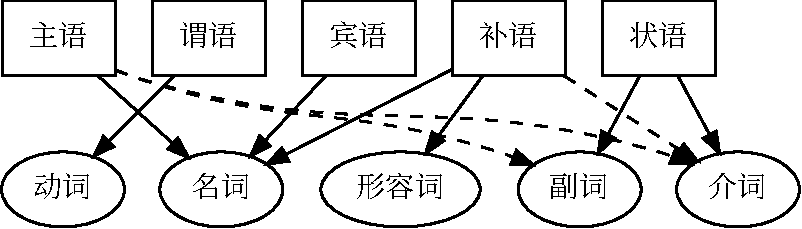
\includegraphics[width=0.7\linewidth]{svo.pdf}
  \caption{\label{fig:svo}句子成分与短语词类对应表}
  \capsource{注:虚线箭头表示在特殊情况下,主语可以是副词短语和介词短语,补语
    可以是介词短语。}
\end{figure}

本章谈的是比较根本的句型问题。虽然简单,却是了解英语语法必要的基础。读者在阅
读英语时不妨详加分析句型,触类旁通,相信会更有收获。


\section{状语}

暂不多讨论状语 Adverbial,其位置多在从句句末,但也可在句首及句中,比较灵活,
可看以下语句先行了解。

\begin{itemize}
\item \unct{My mother}{S} \unct{usually}{A} \unct{enjoys}{V} \unct{parties}{O}
  \unct{very much}{A}。
\item \unct{I}{S} \unct{have been}{V} \unct{in the garden}{A} \unct{all the
    time}{A} \unct{since lunch}{A}.
\end{itemize}
\section{Test}

\textbf{请判断以下各句属于五种基本句型中的哪一种?}

\begin{enumerate}
\item The magician moved his fingers quickly.
\item The police found the letter missing.
\item The police found the missing letter.
\item He ordered himself a steak and a bottle of red wine.
\item Don't you like dancing?
\item The President has gone abroad on a visit.
\item That sounds like a good idea.
\item The box feels heavy.
\item He told his guests a dirty joke at the party.
\item The people elected Bill Clinton President.
\item The child asks her mother a million questions a day.
\item Monkeys love bananas.
\item You can leave the door open.
\item The company has gone bankrupt.
\item Why don't you answer me.
\item I consider you a member of the family.
\item It never rains in California.
\item You 'll look better with these designer glasses on.
\item I can see better without these reading glasses.
\item Do you call me a liar.
\end{enumerate}

\section{其他概念}

普通句子中的补语(COMPLEMENT)(如主语补语、宾语补语) 大家已经了解,夸克引入
了一个相比句法而言更接近于\textbf{词法}的补语:补足
语 (COMPLEMENTATION)\index{概念!补足语 complementation}。
\begin{description}
\item[补足语] 补足语用来\textbf{补充说明}句子中某个成分的词或短语,以使句子的意义更加
  完整。补足语与其他功能,例如状语和名词修饰语有所重叠。

  可以有(包括但不限于):
  \begin{description}
  \item[动词补足语] He deceived \unbf{his father}. [此句中的his father 和主语补语重叠]

  \item[形容词补足语] Tickets are likely \unbf{to be expensive}.

  \item[介词补足语] The pen is \unbf{on the table}.
  \end{description}

\item[递差 (GRADIENCE)] 英语中常常有两个或多个类别之间相近,彼此之间有着不同
  程度级别的差异(级差)。如\ccref{tab:auxverb},\ccref{tab:comparison}等。

  语法解释说明中存在的很多模棱两可、不明确之处多因递差而起。
\end{description}

\chapter{名词短语与冠词}

\textbf{除了主语、宾语、补语这些主要元素外,介词后面所接的宾语往往也是名词短
  语},所以名词短语使用的频率极高。不过名词短语很容易出错,尤其是\textbf{冠
  词}的部分,写作时一不小心就会用错。一般语法书处理这个问题时,通常会列出一长
串规则,再附注一大堆例外,这种语法书,坦白说对于学英语的人并没有太大的帮助。
本章就要和读者一同来探讨名词短语,尤其是冠词的用法。本书中没有规则要背,自然
也就不会有所谓的例外。只要经由理性的探讨,便足以涵盖传统文法所有的规则,而且
更深入、更灵活。

\section{名词短语}

首先,英语是一种拼音文字,和其他\textbf{拼音文字一样,用词尾的变化来表示单、
  复数}。不仅如此,在名词短语的开头,还有一些词或短语来\textbf{配合标示该名词
  有何种所指},是有定的some-, all还是不定的a/an/any- 等,这种词或短语在语言学
上称为\textbf{“限定词”(Determiners)}。它与词尾的单复数符号互相呼应,共
同determine 名词的范围。冠词就是 Determiners 之中的一种。请看下面的例子:

\begin{table}[]
  \centering
  \begin{tabular}{ll}
    \textbf{a new book}         & 一本新书     \\
    \textbf{many good  students} & 许多好学生    \\
    \textbf{his beautiful wife} & 他美丽的妻子   \\
    \textbf{the best answer}    & 最好的答案    \\
    \textbf{those sweet roses}  & 那些芳香的玫瑰花
  \end{tabular}
\end{table}

这几个名词短语都是由三个部分所构成。第一个部分(a, many, his,the, those等)
就是\textbf{限定词},这个限定词决定第三个部分(book、students、wife等),亦即\textbf{名词}部分
的范围。中间的部分(new、good、beautiful等)则是\textbf{形容词},为依附在名词上的修饰
语,是可有可无的元素。

其实,\textbf{名词短语的这三个部分当中,每个部分都可以省略}。在 a new book中,即使拿掉
形容词,剩下 a book,这个名词短语还是正确的。同样地,在 the best answer 中如
果拿掉名词,剩下 the best 也一样是正确的。例如:
\begin{itemize}
\item Of these answers, this one is \unbf{the best}.

  在这些答案中,这个最好。
\end{itemize}

读者可以从此句中清楚了解 the best 就是 the best answer 的意思。甚至在those
sweet roses 中,可以把形容词和名词一起拿掉,只剩下those,仍是正确的名词短语。
比如说,你指着一些玫瑰花,对花店老板说:
\begin{itemize}
\item I want \unbf{those}.

  我要那种的。
\end{itemize}

老板就会知道你要的是什么。

\section{什么时候不需要用限定词?}

如果把 many good students 中的限定词 many 拿掉,剩下 good students,仍然是正
确的。但如果把 a new book 中的限定词 a 拿掉,只剩下new book,就变成一个错误的
名词短语,而这种错误在写作时偏偏常犯,所以我们有必要进一步加以讨论。

从语源学(etymology)的角度来看,冠词 a(n) 可以视为 one一字的弱化(reduction)
结果。也就是说,\textbf{a(n) 就代表 one的意思,只是语气比较弱。} a(n) 与 one同样都
是在交代\textbf{它后面所接的名词是“一个”的概念}。如果后面的名词不适合以“一个”来交
代,也就是不适合加a(n) 的话,就可把限定词这个位置空下来。例如:
\begin{itemize}
\item \unbf{Unmarried men} are a rare species these days.

  未婚男性目前是稀有品种了。
\end{itemize}

在名词短语 unmarried men中,只有形容词(unmarried)和名词(men)两个部分,而
没有限定词。这是因为men 一字已清楚表示名词是复数,自然不能再用 an来表示“一
个”,这时就可以把限定词省略。在 a new book 中,book是单数形态,因此要用限定
词来配合标示它。所以,如果只说 new book,就变成不完整的表示。

除了\textbf{复数}以外,\textbf{抽象名词}(如honesty、bribery)没有具体形状,不能以“一个”来
表示。物质名词(如water、food)虽然是具体的东西,可是\textbf{形状不固定},也不能以“一
个”来表示。\textbf{这些不能以a(n) 来引导的词就可以把限定词省略,即零冠词(the
  zero article)。}例如:

\begin{itemize}
\item  \unbf{Honesty} is not necessarily the best policy.

  诚实不一定是上策。

\item  \unbf{Fresh water} is a precious resource in Saudi Arabia.

  淡水是沙特阿拉伯的珍贵资源。
\end{itemize}

像 honesty 和 water 这些没有复数形态的词,都不适合加a(n)。我们可以这样说:如
果词尾加 ,则表示该名词为复数。如果前面加a(n),则表示“一个”,也就是单数如
果不能加 ,通常表示这个字没有办法数,自然也就不能说是“一个”了。这时候我们
就可以不用限定词。接着我们来处理一个比较复杂的问题:专有名词。

\section{专有名词与补语位置}

人名(如 Genghis Khan)、地名(如Taipei)等都是\textbf{专有名词。因为它所代表的对象
  只有一个,也不适合加a(n),所以可以不用限定词。}为什么只有一个的东西也不能
加 a(n)呢?因为如果用 a Genghis Khan 来代表成吉思汗,那么这里指的是 one
Genghis Khan(一个成吉思汗)的意思。亦即在此句中暗示有第二个成吉思汗存在,所
以才特别需要标示是“一个”。如果只有一个成吉思汗存在,就不必这样标示,只要
说Genghis Khan,大家也就知道在说谁了。加 a(n) 与加 是一体的两面,我们用这两
个符号分别来表示单、复数。\textbf{如果一个名词不能加 \emph{-s}(或者是作不规则复数变
  化),那么它也就不能加 a(n)。专有名词就是如此。}

要判断一个名词是否为专有名词,有时并不是那么容易。像 Sunday这种字,一个月中可
能会有四到五天,所以我们可以说:
\begin{itemize}
\item There are \unbf{five Sundays} this month.

  这个月有五个星期日。
\end{itemize}

这时候它就不算是专有名词。可是在一个星期中星期日只有一天,所以我们也可以说:
\begin{itemize}
\item I have an appointment on \unbf{Sunday}.

  我星期日有约。
\end{itemize}

这时它就是唯一的一天,也就算是专有名词。

实际上,可数与不可数只是根据“不同的\textbf{单位}来实现”(realized by different
lexical items),并无定然。并且是在世俗流变之中,如two cups of coffee在现实中
已可直说two coffees。




放在补语位置的专有名词最难以判断。补语和主语(或宾语)之间有同等的关系,\textbf{如
  果主语(或宾语)是专有名词(例如人名)的话,那么它的补语既然和它同等,便也
  会被当做是专有名词来使用,条件是在补语位置上的名词也必须具有“唯一” 的性
  质。}例如:

\begin{itemize}
\item Mr. Elson was \unbf{president} of the high school.

  埃尔森先生曾是这所高中的校长。
\end{itemize}

本句中 Mr.Elson 是人名,而且没有第二个存在,所以不能加 ,也不能加a,我们就
可以不用限定词。而在补语位置上的 president本来只是个普通名词,并不是只有这所
高中才有校长,而且这所高中的校长历来也不只埃尔森先生一人。因此,“校长”为普
通名词,而“埃尔森先生”为专有名词,两词性质本不相同。可是,因为在此句中“校
长”是埃尔森先生的补语,可以和埃尔森先生划上一个等号,所以可用专有名词来诠释
它。再者,当时这所高中校长一职确实只有埃尔森先生一人,因此也支持这个诠释。所
以president一词没有限定词。这就是把它当作专有名词的结果。再看下例:

\begin{itemize}
\item Some say he was \unbf{a better president} than Mr.Robert.

  有人说他当校长,比罗伯特先生干得更好。
\end{itemize}

在这个从句中,主语 he 就是埃尔森先生。president仍然是主语补语,可是这里就
要加 a了。为什么?因为在上下文中和罗伯特先生做比较,这么一来就有前后两任校长,
可以加 ,不是专有名词了。还有:

\begin{itemize}
\item  Mr.Elson is also \unbf{a member} of the Council of the city.

  埃尔森先生也是该城市政会委员。
\end{itemize}

本句中 a member of the Council 也是埃尔森先生的补语,类似 Council of the
city。可是高中校长同一时间只有一人,\textbf{市政会委员则有很多人},所以 a
member需要交代是“一名”,而非专有名词。

另外,当同位语是补语时,注意是否为专有名词,例如:

\begin{itemize}
\item Martin Wales, \unbf{Head} of the football team, at the time, wore a
  mustache.

  马丁·韦尔斯,当时的足球队长,留有小胡子。
\end{itemize}

句中 Head of the football team 一般称为同位语,其实就是 who was Head of the
football team at the time 这个关系从句的省略。其中 who代表马丁·韦尔斯,
而 Head则是主语补语,和马丁·韦尔斯是同等关系,所以仍然算是专有名词,不必用限
定词。

写主语补语时,要注意该补语是否为专有名词。写宾语补语时也是一样。例如:

\begin{itemize}
\item  Clinton made Gore \unbf{campaign partner} of the Presidential election.

  克林顿选择戈尔为总统大选竞选搭档。
\end{itemize}

句中 campaign partner没有限定词,当专有名词使用。因为它是“戈尔”的宾语补语,
与其为同等关系。而副总统搭档只有一人,所以它便成为专有名词的用法。

\section{定冠词 the 的用法}

在语源学上,\textbf{the 可视为 that 或 those 的弱化形式。}而 that 或 those是指示限
定词,有明确的指示功能\footnote{此外,that, these或 those还可做指示代词。如 This is a
  question. }。所以定冠词 the也可以用同样的角度来了解:凡是上下文中有明指或暗
示时,也就是有“那个”的指示功能时,便要用定冠词the。请比较:

\begin{itemize}
\item  I need \unbf{a book} to read on my trip.

  我在旅途中需要带本书读。
\item  I have finished \unbf{the book} you lent me.

  我已把你借给我的书读完了。
\end{itemize}

在第一句中,a book 只是 one book 或 any book,并没有特别指定是哪一本。在第二
句中,the book 就是 that book,特别指出是“你借我的那本”。因为明指出来,所以
要用定冠词。请再比较:

\begin{itemize}
\item  \unbf{Modern history} is my favorite subject.

  现代史是我最喜欢的科目。
\item  \unbf{The history of recent China} is a sorry record.

  中国近代史是部伤心史。
\end{itemize}

第一句 modern history 一词中,history 是抽象名词,不可数,因而没有a。而在形容
词位置上的 modern 只是附在 history上的修饰语,并不算明确的指示,所以不必
加 the。第二句中 the history of recent China (中国近代史)则有 of recent
China附在后面,用来指出“那一段”历史。因为有这种指示性,所以必须在前面加上定
冠词the,但也不要死背前、后修饰语的差别。再看看下面这一组例子:

\begin{itemize}
\item  He should be home; I saw \unbf{a light in his house}.

  他应该在家;我看见他家亮灯了。

  \begin{description}
  \item[分号 ;] \index{;, 分号} 用以连接两个以上独立句子,但各句之间又有比句号
    更紧密的关系;或者用以分隔并列,但范畴略有差别的部分。
    \begin{itemize}
    \item On our vacation, we visited \textbf{London, England; Paris, France;
        Berlin, Germany; and Rome, Italy}.
    \end{itemize}

  \end{description}

\item  Turn off \unbf{the portal light}.

  把门口的灯关掉。
\end{itemize}

第一句中虽然 a light 后面有 in his house来修饰,可是一栋房子中电灯可能有数十
个,如果看到有一个是亮的,仍然只能算是one light,而不是 that light 。所以 in
his house虽然放在后面,但并不算是明确的指示,仍然要用 a light。相反的,在第二
句中,叫人把大门口的灯关掉,在 the portal light一词中的portal,虽然是附在名词
前面的形容词,可是有明确的指示功能,因为门口的灯通常只有一盏,所以已经指明了
要关哪一盏灯,这时就要用the light。总之,不必死背,但要先了解 a(n) 是来自
于 one(一个),the则是来自于 that/those(那个),再逐一判断。

另外,如果上下文中没有明确指出来,但有\textbf{清楚的暗示},仍然要用定冠词the。例如,
先生对太太说:
\begin{itemize}
\item  I'm going to \unbf{the office} now.

  现在我要去办公室。
\end{itemize}

虽然 the office后并没有明指,可是太太知道,就是老公上班的办公室,这时还是要
用 the。再看下例:
\begin{itemize}
\item  Do you mind if I open \unbf{the window}?

  我可以把这扇窗户打开吗?
\end{itemize}

当有人在公共汽车上向你这么说时,虽然在 window前后没有指示性的字眼,可是对话的
情境清楚暗示“就是你旁边这扇窗户”,所以这时候还是要用the 。如果用 a,就变
成:
\begin{itemize}
\item  Do you mind if I open \unbf{a window}?

  我可以打开一扇窗户吗?
\end{itemize}
这时的意思便成为 any window,也就是对方要在整个公共汽车数十扇窗户中,随便挑一
扇来打开,却先来征求你的同意。虽然这不是不可能,却是很奇怪的讲法。


\section{定冠词与专有名词}

\textbf{专有名词的定义是:只有一个对象存在的名词},像 Genghis
Khan 和 Taipei等。既然只有一个对象存在,就没有“这个”、“那个”的分别,也
就\textbf{不能加定冠词the}。如果你说 this book,则暗示还有 that book 的存在,
这时就需要指明是this book,也就是 the book。像 Taipei这种字就不能这样使用。所
以,专有名词和定冠词是有冲突、且不能并存的。如果加了the,就表示这个东西有两个
以上,也就不是专有名词了。例如:

\begin{itemize}
\item  This is not \unbf{the John Smith} I know.

这不是我所认识的约翰·史密斯。
\item  This is a photography show of \unbf{the Taipei} 50 years ago.

这是表现 50 年前的台北的摄影展。
\end{itemize}

第一句暗示还有另一个约翰·史密斯存在,或是他有另外一面,是我所不认识的。这时
有两个约翰·史密斯存在,所以“约翰·史密斯”就不再是专有名词,可以
用this 或 that 来区分,这也就是为什么写 the John Smith的原因了。还有,“50年
前那个台北”这句话暗示和今日台北不同了,有两个台北。这时台北也就成了普通名词,
可以指来指去,所以要用the Taipei 50 years ago 来表示。

最后,在许多语法书上被列为例外,并要求学生背下来的东西,其实都非例外,反而都
是很容易了解的。比如,\textbf{一般语法书列出海洋、河流、群岛、群山、杂志名、船名等
  等,说这些是“要加定冠词的专有名词”,是例外。}但是,这种说法并非完全正确。
首先,这些清单并不周全。而且,大部分的人不是懒得背,就是背不下来。死背不但不
能变通,一碰到变化还是不会。现在我们就来看看这些所谓的例外:

\begin{longtable}[]{@{}ll@{}}
  \textbf{the Pacific (Ocean)} & 太平洋 \\
  \textbf{the Atlantic (Ocean)} & 大西洋 \\
  \textbf{the Indian Ocean} & 印度洋 \\
  \textbf{the Mediterranean (Sea)} & 地中海 \\
  \textbf{the Dead Sea} & 死海 \\
\end{longtable}

在“太平洋” the Pacific (Ocean) 一词中,Pacific是放在形容词的位
置,\textbf{字尾 \emph{-ic} 是明显的形容词字尾}。在名词位置上的 Ocean其实是\textbf{普通名词}(世
界上有三个洋。只要有两个以上就不算是专有名词),在此被省略掉。所以\textbf{定冠词the
  是配合后面的普通名词 Ocean},指出“叫做 Pacific的那个洋”。这是规规矩矩的用法,
完全没有例外。在三大洋中只有印度洋不适合省略,因为the Indian 可能会被误解
为“这名印第安人”。同理, the Mediterranean (Sea) 是普通名词 the sea 加上形
容词Mediterranean,也不是例外。“地中海”可以省略sea,因为省略之后仍然够清楚。
但“死海” the Dead Sea就不能省略,否则会被误会为“死人” the dead people。再
看下面的例子:

\begin{itemize}
\item  the Philippine Islands → \unbf{the Philippines}

菲律宾群岛
\item  the Alp Mountains → \unbf{the Alps}

阿尔卑斯山
\end{itemize}

这两个复数的“群岛” Islands、“群山” Mountains,也是普通名词。可是名词部分
被省略掉,以形容词位置取代之,并且把复数的  移到前面来。这也不是例外,只是
很合理的\textbf{省略方式}罢了。同样的:

\begin{longtable}[]{@{}ll@{}}
  \textbf{the Mississippi (River)} & 密西西比河 \\
  \textbf{the Titanic (Ship)} & 泰坦尼克号 \\
  \textbf{the Hilton (Hotel)} & 希尔顿饭店 \\
  \textbf{the Times (Newspaper)} & 希尔顿饭店 \\
\end{longtable}

如果把这些名词短语的第三个部分还原,即可看出\textbf{它们的名词位置都是普通名
  词,所以都可以加冠词。}而所谓的专有名词都是放在\textbf{形容词位置的修饰语},
所以并不是什么例外,请看下面的例子:

\begin{longtable}[]{@{}ll@{}}
  \textbf{the United States} of America& 美国 \\
  \textbf{the United Nations} & 联合国 \\
\end{longtable}

这两个例子中,在名词位置的其实都是普通名词(States,Nations),皆可加冠词。只有
America 这个名词短语是专有名词,所以前面没有加冠词。

以上的叙述中,重要观念有三:

\textbf{一、名词短语包括限定词、形容词、名词三个部分。任一部分都可能省略。}

\textbf{二、如果名词短语中不用限定词,是因为该名词不适合加 a(n)。}

\textbf{三、a(n) 是 one 的弱化结果,而 the 是 that/those 的弱化结果。}

冠词的问题基本上是写作时容易碰到的问题,阅读时要多加观察。在看文章的时候请留
心名词短语,尤其是冠词的用法,就是最好的练习。

\section{Test}


\textbf{请选出最适当的答案填入空格内,以使句子完整。}

\begin{enumerate}
\item The carpenter repaired \ttu.
  \begin{tasks}(2)
    \task the table's legs
    \task table's legs
    \task legs of the table
    \task the legs of the table
  \end{tasks}

\item Mr. Smith has three \ttu under his name.
  \begin{tasks}(2)
    \task shoe stores \task shoes stores \task shoe store \task shoestores
  \end{tasks}

\item The house sits on a \ttu road.
  \begin{tasks}(2)
    \task twelve feet in width
    \task of twelve feet
    \task twelve-foot-wide
    \task twelve-feet
  \end{tasks}

\item These men and women are all \ttu .
  \begin{tasks}(2)
    \task language's teachers \task languages teachers
    \task language teachers \task languages' teacher
  \end{tasks}

\item He ordered  \ttu for breakfast.
  \begin{tasks}(1)
    \task orange juice, bread and butter, coffee, and bacon, and eggs
    \task orange, juice, bread, and butter, coffee and bacon and eggs
    \task orange juice, bread and butter, coffee, and bacon and eggs
  \end{tasks}

\item The prime minister is the real ruler and the prince is merely \textbf{a} \ttu .
  \begin{tasks}(4)
    \task little
    \task small
    \task nobody
    \task none
  \end{tasks}

\item Living in the city, he was always being annoyed by noises of  \ttu .
  \begin{tasks}(2)
    \task one sort of other
    \task one sort of the other
    \task one sort or another
    \task one or others sorts
  \end{tasks}

\item Writing is one thing and talking is quite \ttu .
  \begin{tasks}(2)
    \task the other
    \task another
    \task others
    \task the others
  \end{tasks}

\item The majority of the Members of Parliament are men, but there are  \ttu  women, of course.
  \begin{tasks}(2)
    \task few
    \task little
    \task any
    \task quite a few
  \end{tasks}

\item  \ttu  is what he said: Don't go out!
  \begin{tasks}(4)
    \task This
    \task That
    \task The
    \task These
  \end{tasks}

\item Whether you serve coffee or tea doesn't matter;  \ttu  will do.
  \begin{tasks}(4)
    \task any \task either \task some \task all
  \end{tasks}


\item As we have finished the first chapter, now we will read  \ttu .
  \begin{tasks}(2)
    \task second \task the second \task second one \task the two
  \end{tasks}

\item \textbf{He has two daughters; one is a singer and \ttu  an actress.}
  \begin{tasks}(2)
    \task another \task other
    \task the other \task the others
  \end{tasks}

\item He asked if eighty dollars was enough, and I said that  \ttu twenty would
  do.
  \begin{tasks}(2)
    \task more \task another \task other \task the other
  \end{tasks}

\item Mary Kurt, \ttu  of the troupe, was strongly against smoking.
  \begin{tasks}(4)
    \task alto \task the alto \task an alto \task altos
  \end{tasks}

\item This kind of ball-pen holds  \ttu ink than that.
  \begin{tasks}(4)
    \task less \task fewer \task much \task little
  \end{tasks}

\item \textbf{John works harder than  \ttu boy in his class.}
  \begin{tasks}(2)
    \task all other \task any other \task all the other \task any
  \end{tasks}

\item I was told to take the pills  \ttu six hours.
  \begin{tasks}(2)
    \task each \task every \task other \task the other
  \end{tasks}


\item The man was badly wounded, but there could still be  \ttu  hope.
  \begin{tasks}(4)
    \task little \task few \task a little \task a few
  \end{tasks}

\item  \ttu  these people are going to the concert.
  \begin{tasks}(2)
    \task The most \task Most of \task Most \task Almost
  \end{tasks}

\end{enumerate}

\section{Answer}

\begin{enumerate}


\item (D) 所有格有两种表示方式:人与其他生物可用 's 的形式,无生物则用 of... 的
  介词短语形式来表示。本题的 table 是无生物,故只能从 C 和 D 之间选择。因为
  有 of the table 修饰前面的 legs,表示出来是“哪些”脚,所以要有定冠词 the。

\item (A) 复合名词,前面的名词 shoe 放在\textbf{形容词位置},只能用单数。后面的 store 要用
  复数,因为有限定词 three。D 的 shoestores 是错误拼法,两个词不能连起来。

\item (C) \textbf{名词短语}冠词(a)与名词(road)之间是\textbf{前置修饰语位
    置},而且\textbf{只能放一个“重量”较轻的单词,不能放短语}(详
  见\cref{subsubsec:inversionadj}),故从 C 和 D 来选。既然是形容词,没有复数
  可言,故排除掉 D。

  另外数字+名词+名词用于\textbf{测量},数字通常用\textbf{en dash连字
    符 (--)}连接到第一个名词上。请注意,在这些情况下,\textbf{第一个名词通常
    是单数形式}。

  例外有:
  \begin{description}
  \item[that savings bank] saving常作“节省”或“挽救”之意;savings作“储蓄”之意。

  \item[several clothes hangers] 几个衣架,单数的 cloth 意思是“布”,必须拼成复数 clothes 才是“衣服”的意思。

  \item[your sports car] 当谈论体育或一般的运动时,在英式英语中通常是不可数
    的sport,而在北美英语中则是复数的sports。然而,\textbf{在另一个名词之前,复数
      形式sports在英式英语和北美英语中都有使用}。

  \item[damages negotiations]  赔偿谈判,单数的 damage 意思是“损害”、复数的damages才是“赔偿”。
  \end{description}

\item “语言教师”是复合名词,故由 B 和
  C 之间来选。前面 language 的位置是形容词位置,没有复数,故选 C。

\item bread and butter(奶油吐司)是一种食品,两个词都不可数,不需要限定词,构成
  一个名词短语,因而中间不能有逗号。bacon and eggs (火腿蛋)亦然。这里
  的 bacon 不可数,eggs 是复数,亦不需要限定词。

\item \textbf{(C)nobody 意为“无名小卒”时应作普通名词看待,可加冠词 a。A 和 B 都是形
    容词,不应置于冠词 a 后面当作名词用。}none 是 no one 的复合字,其中
  的 \textbf{no 就是限定词},所以前面不能再加冠词 a。

\item (C) one sort or another 表示 one sort or another sort,是一个常用的短语,
  意为“各种各样的”。

\item (B) 以 another(后面省略 thing)和 one thing 相对,可以表示“不同的两件
  事”,也是常用短语。

\item (D) C 的 any 只适用于否定句或疑问句。肯定句中的 any 要解释为“任何”,在此
  亦不适合。B 的 little 要配合不可数名词才能用。在 A 与 D 之间,few 是否定的
  意味,a few 才能表示肯定,而 quite a few 则是加上强调语气的副词 quite 来表
  示“还不少”。上下文要求肯定语气(由连接词 but 可看出),故选 D。

\item (A) 用来表示上文讲过的一句话,可以用 this 或 that 作代名词。例如:There's
  going to be a raise. Isn't this(或 that) great? 可是,如果代表下文要说的
  一句话,就只能用 this。

\item (B) 两者(coffee,tea)之间任选其一,应用 either,三者以上才用 any。

\item (B) the second 代表 the second chapter,与上文的 the first chapter 对称。

\item (C) 上文有交待一共是两个女儿,除去唱歌的那个,剩下的“那一个”是演员。句意
  中已指明哪一个,所以要用定冠词。the other 后面省略掉 is。

\item (B) 80 元当中已有四个 20(或四张 20 元钞票)了,所以说“再来一个 20(another 20)就够了。”意思是凑成 100。

\item (A) 空格位置是主语 Mary Kurt 的同位语,这个位置倾向于当专有名词看待。再加
  上这个乐团的女低音只有一人,符合专有名词的要求,因而不用冠词

\item (A) ink 不可数,故可排除 B。再从 than that 来看,应是比较级,故排除 C 和 D。

\item (B) 空格后面的 boy 是单数,所以排除复数的 A 和 C。英语的比较级要求较严格:
  只能说比班上“别的”同学用功,不然会造成“包括比自己用功”的语病,所以要
  有 other 一词来限定范围。

\item (B) 多久一次,像 every day,every week,every two months,every
  century(相当于 every hundred years)—样,要用 every 这个限定词来表
  示。six hours 固然是复数,可是像 hours,miles,pounds 这种代表“单位”的字
  眼也可以当单数使用,例如:Three miles is a long way to walk. 所以 every
  six hours 并无冲突。

\item (C) hope 不可数,所以从 A 和 C 来选。上下文要求用肯定语气:“还有希
  望”(从连接词 but 可以看出),所以用表示肯定的 a little。如果用 A,成
  为 little hope,只能表示否定语气:“希望渺茫”。


\item (B) 空格后面有完整的名词短语,已经有限定词 these,所以不能直接再加限定
  词 most 在前面(most 在此并非表示“最”的副词,而是表示“大部分”的限定词),
  只能用介词 of 隔开。而且 most 在此既非一般解释为“最”的最高级,前面也就
  不应用定冠词 the。

\end{enumerate}

\section{不规则名词复数}

以下是规律总结,详表请见\ccref{tab:irrnoun} 。

\begin{description}
\item[以f或fe结尾] 大多数以f或fe结尾的名词的复数形式时将其转为ves:
  \begin{taskitem}(3)
    *  calf -- calves
    *  elf -- elves
    *  half -- halves
    *  hoof -- hooves
    *  knife -- knives
    *  leaf -- leaves
    *  life -- lives
    *  loaf -- loaves
    *  scarf -- scarfs/scarves
    *  self -- selves
    *  sheaf -- sheaves
    *  shelf -- shelves
    *  thief -- thieves
    *  wife -- wives
    *  wolf -- wolves
  \end{taskitem}

\item[元音] 有些名称的复数形式是改变它们的元音声:
  \begin{taskitem}(3)
    *  fireman -- firemen
    *  foot -- feet
    *  goose -- geese
    *  louse -- lice
    *  man -- men
    *  mouse -- mice
    *  tooth -- teeth
    *  woman -- women
  \end{taskitem}


\item[古英语] 有些是沿用古英语:
  \begin{taskitem}(3)
    *  child -- children
    *  ox -- oxen
  \end{taskitem}


\item[以o结尾] 见下文:

  \textbf{有的加``s''}

  \begin{taskitem}(3)
    *  auto -- autos
    *  kangaroo -- kangaroos
    *  kilo -- kilos
    *  memo -- memos
    *  photo -- photos
    *  piano -- pianos
    *  pimento -- pimentos
    *  pro -- pros
    *  solo -- solos
    *  soprano -- sopranos
    *  studio -- studios
    *  tattoo -- tattoos
    *  video -- videos
    *  zoo -- zoos
  \end{taskitem}

  \textbf{有的则加``es''}

  \begin{taskitem}(3)
    *  echo -- echoes
    *  embargo -- embargoes
    *  hero -- heroes
    *  potato -- potatoes
    *  tomato -- tomatoes
    *  torpedo -- torpedoes
    *  veto -- vetoes
  \end{taskitem}

  \textbf{有的两种都可以}
  \begin{taskitem}(2)
    *  buffalo -- buffalos/buffaloes
    *  cargo -- cargos/cargoes
    *  halo -- halos/haloes
    *  mosquito -- mosquitos/mosquitoes
    *  motto -- mottos/mottoes
    *  no -- nos/noes
    *  tornado -- tornados/tornadoes
    *  volcano -- volcanos/volcanoes
    *  zero -- zeros/zeroes
  \end{taskitem}

\item [不变] 拼写不变

  \textbf{单复数同型}:
  \begin{taskitem}(3)
    *  cod -- cod
    *  deer -- deer
    *  fish -- fish
    *  offspring -- offspring
    *  perch -- perch
    *  sheep -- sheep
    *  trout -- trout
  \end{taskitem}

  注:很多鱼类的复数形式都是不变的,但有例外

  \textbf{本身就是复数,只有复数形式}:
  \begin{taskitem}(4)
    *  barracks
    *  crossroads
    *  dice
    *  gallows
    *  headquarters
    *  means
    *  series
    *  species
  \end{taskitem}

\item[借用] 单词和其复数形式都借用自其他语言:

  \begin{taskitem}(3)
    *  alga -- algae
    *  larva -- larvae
    *  vertebra -- vertebrae
  \end{taskitem}

  \textbf{以``us''结尾的转为``a''(适用于专业术语)}:
  \begin{taskitem}(3)
    *  corpus -- corpora
    *  genus -- genera
  \end{taskitem}

  \textbf{以``us''结尾的转为``i''}:
  \begin{taskitem}(3)
    *  alumnus -- alumni
    *  bacillus -- bacilli
    *  focus -- foci
    *  nucleus -- nuclei
    *  radius -- radii
    *  stimulus -- stimuli
    *  syllabus -- syllabuses
    *  terminus -- termini
  \end{taskitem}

  \textbf{以``um''结尾的转为``a''}:
  \begin{taskitem}(3)
    *  addendum -- addenda
    *  bacterium -- bacteria
    *  datum -- data
    *  erratum -- errata
    *  medium -- media
    *  ovum -- ova
    *  stratum -- strata
  \end{taskitem}

  \textbf{以``is''结尾的转为``es''}:
  \begin{taskitem}(2)
    *  analysis -- analyses
    *  axis -- axes
    *  basis -- bases
    *  crisis -- crises
    *  diagnosis -- diagnoses
    *  emphasis -- emphases
    *  hypothesis -- hypotheses
    *  neurosis -- neuroses
    *  oasis -- oases
    *  parenthesis -- parentheses
    *  synopsis -- synopses
    *  thesis -- theses
  \end{taskitem}


  \textbf{以``on''结尾的转为``a''}:
  \begin{taskitem}(2)
    *  criterion -- criteria
    *  phenomenon -- phenomena
    *  automaton -- automata
  \end{taskitem}


  \textbf{意大利语,变``o'' 为 ``i''}:
  \begin{taskitem}(3)
    *  libretto -- libretti
    *  tempo -- tempi
    *  virtuoso -- virtuosi
  \end{taskitem}

  \textbf{希伯来语,末尾加 ``im''}:
  \begin{taskitem}(3)
    *  cherub -- cherubim
    *  seraph -- seraphim
  \end{taskitem}

  \textbf{希腊语,末尾加ta}:
  \begin{taskitem}(3)
    *  schema -- schemata
  \end{taskitem}
\end{description}

\section{限定词}
\label{sec:determin}

\subsection{前中后位限定词}

名词短语中,限定词位置大体可以分为前位、中位、后位(见\cref{tab:determ})。
\index{概念!限定词!前位}\index{概念!限定词!中位}\index{概念!限定词!后位}

\begin{table}[htbp]
  \centering \small
  \begin{talltblr}[ caption = {名词短语中限定词的位置},
    label = {tab:determ},
    ]{
      width=0.9\linewidth, colspec={lX},
      rowsep=2pt, colsep=4pt,
    }
    \toprule
    \SetCell[c=2]{l} \textbf{前位限定词\qquad (互斥,只选其一)}& \\
    感叹 & such, what\\
    倍数词 & double, twice, three times\\
    分数词 & one-third, one-fifth\\
    数量词 & all, both, half\\
    \midrule
    \SetCell[c=2]{l} \textbf{中位限定词\qquad (互斥,只选其一)} & \\
    冠词 & a, an, the\\
    物主代词 &  my, our, your, his, her, its, their\\
    名词所有格 & the rabbit's, the wolf's\\
    关系代词 & whose,which\\
    指示代词 & this, that‍‍, these, those\\
    wh-ever 限定词 & whichever, whatever, whoever\\
    疑问代词 & what, whose,which\\
    不定代词 & {enough, each, every, some, any, either, neither,\\
      lot(s)/piece/few/plenty of, no}\\
    \midrule
    \SetCell[c=2]{l} \textbf{后位限定词}  \\
    基数词 & one,two,three\\
    数量词 & {few, little, many, much, several\\ large/great/good
      number of} \\
    (一般)序数词 & {first, second, fourth, twentieth,\\ next, last, past, (an)other}\\
    \bottomrule
  \end{talltblr}%
\end{table}

\textbf{限定词互斥的例外:}
\begin{itemize}
\item 中位限定词\textbf{every}有时可在属格后面,例:

  His every action shows that he is a very determined young man.
\item 前位限定词 such 用作代用式 (pro-form)时,也能接在数量词 any, no 和 many 以
  及基数词的后面:

  no/any/several/many/forty-one such incidents \ldots
\end{itemize}


除作前位限定词外,all, both 和 half 作为代词还能带 of- 短语 (partitive
of-phrase)表示“部分”。 \textbf{与名词连用时, of- 短语可有可无,与代词连用则非
  用 of短语不可}:
\begin{taskitem}(2)
  * all (of) the students
  * all of them/whom
  * both (of) his eyes
  * both of them/which
  * half (of) the time/cost
  * half of it/this
\end{taskitem}


\subsection{类指}

以下用法可表示\textbf{类指}\index{类指}:
\begin{description}
\item[a + 可数名词单数] 如 \textbf{a tiger} (\textbf{不定指}).
\item[the + 可数名词单数] 如 \textbf{the tiger}(\textbf{定指})。
\item[可数名词复数] 如 \textbf{tigers}(\textbf{不定指})。
\item[零冠词 + 不可数名词] 如 milk.
\end{description}

\textbf{如果类指整个群体里的所有成员,就不能用 a/an 。}
\begin{itemize}
\item \unbf{The tiger} is in danger of becoming extinct.

  整个老虎种族,不能用a tiger,只能用the tiger is 或者 tigers are。

\item Do you like \unbf{horses}?

  直接用可数名词复数类指,是最常见的。
\end{itemize}

\textbf{另外名词短语作非主语时,只有the + 单数 仍保持其类指功能。}
\begin{itemize}
\item Nova has been studying \unbf{the medieval mystery play}.

  诺娃正在学习中世纪神秘剧。如将the替换成a,则是一种。如用复数则可能是部分。
\end{itemize}

\section{属格}

\subsection{归属于:属格和of结构}


\begin{description}
\item[the genitive] 属格(所有格):名词或者形容词,used to show possession or
  close connection between two things. 展示两者之间的所属或紧密关系。
\item[of-construction] of介词 + 名词性短语,belonging to sb/sth; relating to sb/sth 属于(某人/某物);关
  于(某人/某物)。
\end{description}

\begin{itemize}
\item What is \unbf{the ship's} name?

  What is the name \unbf{of the ship}?

\item Some people's opinions

  the options of some people (不很清晰,少用)
\end{itemize}
许多情况下,这两种形式意义相同且完全能够成立。

属格和of结构应根据如下侧重点,结合实际情况加以选择:
\begin{enumerate}
\item \textbf{具有人性特点的名词类别常常用属格。}例如人、高等动物、集体(多个个人组
  成)、地理位置(人类生活区域)、时间、人的感官活动等。
  \begin{taskitem}(2)
    * the nations resources
    * Europe's future
    * China's development
    * the school's history
    * today's paper
    * a day's work
    * the body's needs
    * the game's history
  \end{taskitem}

\item \textbf{属格有特指的意思,带有限定性;of结构有泛指的意思。}
  \begin{itemize}
  \item Susan's son (苏珊的儿子,单看短语本身她也只有一个儿子)

  \item a son of Susan (苏珊有多儿子,其中之一)
  \end{itemize}

\item 根据\textbf{末尾焦点 (end focus) 和末尾重心 (end-weight)原则。}更复杂和
  重要的单位应放在名词短语末尾。这样一来,\textbf{属格倾向于将信息中心放在名
    词中心词上,of结构倾向于将中心放在介词补足语上。}

  \begin{itemize}
  \item The explosion damaged \unct{the ship's funnel}{焦点在funnel}.
  \item The explosion damaged \unct{the funnel of the ship}{焦点在ship}.

    爆炸损坏了船上的烟囱。

  \item the ears of the man in the deckchair. 根据尾重,避免隔断产生歧义

    帆布躺椅上那个男人的耳朵。
  \item \sout{the man's ears} in the deckchair. [歧义,惊悚]

    帆布躺椅上有那个男人的耳朵。
  \end{itemize}

\item 两者皆可的情况下,属格往往比较简明清晰,优先考虑。
\end{enumerate}

\subsection{独立属格 (THE INDEPENDENT GENITIVE)}

如果上下文中已交代清楚属格后面的中心词,则中心词可以省略。省略的结果就构成了
所谓“\textbf{独立属格}”。\index{概念! 独立属格 the independent genitive}
\begin{itemize}
\item  My \unbf{car} is faster than \unbf{John's}.  [省略 car]
\item  Her \unbf{memory} is like \unbf{an elephant's}. [省略memory]
\item \unbf{Mary's} was the prettiest \unbf{dress}. [省略dress]
\item If you can't afford a \unbf{sleeping bag}, why not borrow \unbf{somebody
    else's}? [省略sleeping bag]
\item The New York's \unbf{population} is greater than \unbf{Chicago's}.
\end{itemize}

需要注意,of结构如果出现在可比较语境 (comparable environments)中,of前面通常
要加指示代词\textbf{that/those}。上句如采用of结构,应是
\begin{itemize}
\item The \unbf{population} of New York is greater than \unbf{that of Chicago}.
\end{itemize}

\subsection{后置属格(双重属格)}

\begin{description}
\item[后置属格] 将本应前置的\textbf{人的属格后置},并在其前加\textbf{of},也称双重属
  格。
\end{description}

相比于正常属格,后置属格的限定性弱一些。
\begin{itemize}
\item some friends \unbf{of Jim's}

  等同于 some \unbf{Jim's} friends,将Jim's 后置并在前面加of

\item several students \unbf{of his}

  等同于several \unbf{his} students,将 his 后置并在前面加of
\end{itemize}

后置属格可能是古英语传承自其他语言的遗留,与当前语法有些不同之处,很难简明扼
要说清楚。

当中心语为人称,即人称 + of + 后置修饰语 时,后置修饰语可以不用属格。
\begin{itemize}
\item A\xout{/The} friend of \unbf{Jim('s)} is coming to the party.
\end{itemize}

注意,因中心语是被of短语后置修饰的,不能定指或专有,所以不能用The:
\begin{itemize}
\item \sout{Mary of Mrs Brown} [误,被MRs Brown修饰的Mary本来就定指确定的。]

\item Mrs Brown's Mary
\end{itemize}

试分析下组例子中的不同含义:
\begin{itemize}
\item a painting of my sister's. [我姐妹画的,或者属于我姐妹的,一幅画]
\item a painting of my sister. [画有我姐妹的一幅画]
\item a painting by my sister. [我姐妹画的一幅画]
\item a painting of my sister by my brother. [我兄弟画有我姐妹的一副画像]
\end{itemize}


后置属格在中国英语应试教育中时有出现……

\subsection{带 of- 短语的同位关系}

有些名词短语中含有一个介词短语成分。而起介词短语并非正规的后置修饰语,而
是\textbf{前面名词的同位语}。这种结构由“限定词+名词 (N2) + of + \textbf{不定
  冠词} + 名词 (N1) 构成,

\begin{itemize}
\item the city \unbf{of Rome}

  等同于:

  Rome \emph{is} a city.

  The city \emph{(that I mean) is} Rome.

\item the news of the team's victory

  the news \emph{was} the team's victory
\end{itemize}


\section{平行结构}

如果两个名词一起放在同一平行结构里,即使是单数具数名词,也有\textbf{省略冠词}的倾向:
\begin{taskitem}(4)
  * face to face
  * day by day
  * hand in hand
  * eye to eye
  * arm in arm
  * mile upon mile
  * back to back
  * side by side
\end{taskitem}

有时一个名词与另一个具有相反意义的名词相平衡,如;
\begin{taskitem}(2)
* from father to son
* husband and wife
* from (the) right to (the)left
* from (the) beginning to (the) end
* both mother and child
* neither child nor adult
\end{taskitem}

这些平衡结构中的名词基本上部会有数的变化,也不可能有限定词和修饰
语,\textbf{实际上是习语},是冠词“固定“用法的例子。

\textbf{带有名词重复的短语通常具有副词功能。}


\chapter{代词}

代词更多情况下不是简单“代替”名词,而是代替“名词性短语”。

\section{人称代词}

\begin{table}[htbp]
  \centering \small
  \begin{talltblr}[ caption = {人称代词的主格、宾格、属格以及反身代词},
    label = {tab:whoself},
    note{a} = {限定式属格:在名词短语中起限定作用,修饰其后的中心语。},
    note{b} = {独立式属格:省略场景中已知要修饰的名词,独立使用。},
    ]{
      width=\linewidth, colspec={llllllllll},
      rowsep=1pt, colsep=2pt,
      row{1} = {font=\bfseries, c},
    }
    \toprule
    & \SetCell[c=4]{m}单数 & & & & \SetCell[c=2]{m}复数 & & \SetCell[c=2]{m}单复数 & \\ \midrule
    主格 & I & he & she & \SetCell[r=2]{m} it & we & they & \SetCell[r=2]{m} you & who \\
    宾格 & me & him & her & & us & them & & who(m) \\
    反身代词 & myself & himself & herself & itself & ourselves & themselves
    & {yourself \\ yourselves} & -- \\ \midrule
   \SetCell[c=3]{m} \textbf{属格(物主代词)} &&&&&&&&&\\
    限定式 & my & \SetCell[r=2]{m} his & her & \SetCell[r=2]{m} its & our & their & your &  \SetCell[r=2]{m} whose \\
    独立式 & mine & & hers & & ours & theirs & yours & \\
    \bottomrule
  \end{talltblr}%
\end{table}

宾语位置如是人称代词,则使用人称代词宾格,这个大家一般都了解。但\textbf{主语
  补语,在正式文体中使用主格,在非正式文体中使用宾格且越来越流行。}

\begin{enumerate}
\item \unct{It}{S} \unct{was}{V} \unct{he}{$\mathbf{C_S}$}.

  非正式文体中,不用he,而用him。

\item  \unct{It}{S}\unct{'s}{V} \unct{I}{$\mathbf{C_S}$} who's to blame.

  我负有(不好的)责任。非正式文体中,变 I为me.
\end{enumerate}

He is$ \left\{
  \begin{aligned}
    &\text{more intelligent than} \\
    &\text{as intelligent as}
  \end{aligned}
\right\} $ \unbf{she (is)}.

用主格she的话,加is更符合并列连接的语义。非正式文体中,变she 为her.

\section{代用的it}

由于 it 是人称代词中最中性的而且在词义上是无标记的,它就用来作为“\textbf{虚
  主语}”或“\textbf{代用主语}”,尤其用在那些表示时间、距离或天气情况的词组中:
\begin{itemize}
\item What time is it?
\item How far is it to York?
\item It's warm today.
\item It's getting dark.
\end{itemize}

也许完全虚指或无所指it 的最好的例子是在下列习语中。 it在这些习语中接在动词后
面,笼统地泛指“生活”等:
\begin{itemize}
\item At last we've made \unbf{it}. [achieved success]
\item have a hard time of \unbf{it}. [to find life difficult]
\item How's \unbf{it} going?
\item Go \unbf{it} alone.
\item You're in for \unbf{it}. ["You're going to be in trouble."]
\end{itemize}

it 也能用来\textbf{代替谓体 (PREDICATION)},尤其是\textbf{代替表示特征的补语}。
She was$ \left\{
  \begin{aligned}
    &\text{a rich woman} \\
    &\text{rich}
  \end{aligned}
\right\} $  and she looked \unbf{it}.

上句it 指代前面谓体 a rich woman 或者 rich。

\section{反身代词}

反身代词以 \emph{-self} (单数) 和 \emph{-selves} (复数)结尾(
见\cref{tab:whoself})。顾名思义,反身代词“反映“从句或句子中另一个名词性成
分(通常是主语),并与它形成互指关系:
\begin{itemize}
\item She allowed herself a rest.
\item He is not himself today.
\end{itemize}

\begin{table}[htbp]
  \centering \small
  \begin{talltblr}[ caption = {反身代词的功能},
    label = {tab:reflexive},
    ]{
      width=\linewidth, colspec={ccl},
      rowsep=2pt, colsep=4pt,
      row{1} = {c, font=\bfseries},
    }
    \toprule
    先行词        & 反身代词        & 举例            \\ \midrule
    \SetCell[c=2]{l,m} \textbf{基本用法} &                    &         \\
    主语         & 直接宾语        & \unbf{They} helped \unbf{themselves}.     \\
    主语         & 间接宾语        & \unbf{She} allowed \unbf{herself} a rest. \\
    主语         & 主语补语        & \unbf{He} is not \unbf{himself} today.    \\
    主语         & 介词补足语       & \unbf{Jim} pay for \unbf{himself}.        \\\midrule
    \SetCell[c=2]{l,m} \textbf{强调用法} &                   &          \\
    主语         & 同位语短语       & \unbf{We} couldn't come \unbf{ourselves}. \\
    主语         & 同位语短语       & \unbf{We} \unbf{ourselves} couldn't come.\\
    \bottomrule
  \end{talltblr}%
\end{table}

当一个非限定性从句 (NON-FINITE CLAUSE) 或一个名词化短语有一个以\textbf{最不确
  定的人 (``someone or other'') }作隐含主语时,可用反身代词
\textbf{oneself}(或用它在非正式文体中的等同词 \textbf{yourself})。
\begin{itemize}
\item Voting for \unbf{oneself} is unethical.

  给自己投票是不道德的。(非正式文体中可用yourself)
\end{itemize}

如涉及到自身,以下介词后面必须用反身代词:
\begin{taskitem}
  * look at/after
  * do with
  * thinks of
  * take upon
  * a story about
  * portraits/photograph of
\end{taskitem}

\section{前指、后指、实景所指和先行词}
\label{sec:anacata}

\begin{description}
\item[实景所指 (SITUATIONAL REFERENCE)] \index{概念!实景所指situational reference}指语言外的实际环境,如双方都心照不宣或被指向的人和
  物。
\item[前指 (ANAPHORIC REFERENCE)] \index{概念!前指anaphoric reference}代词或
  其他指代词与\textbf{上文中}的名词性话语形成互指关系。
\item[后指 (CATAPHORIC REFERENCE)] \index{概念!后指cataphoric reference}代词
  或其他指代词与\textbf{下文中}的名词性话语形成互指关系。
\item[先行词 (ANTECEDENT REFERENCE)] \index{概念!先行词antecedent reference}与代词或其他指代词形成互指关系的那部分名词性话语。
\item[近指] \index{概念!近指}既可以前指也可以后指的指示代词,如this/these.
\item[远指] \index{概念!远指}只可以前指的指示代词,如that/those.
\end{description}

\begin{itemize}

\item He told the story like \unbf{this}: ``Once upon a time \ldots{} ''

  因直接引述的话语在句子后面,只能使用近指的this,而不能用that.

\item What do you think of TH\`{A}T! Bob smashes up my car, and then expects me to
  play for the repairs.

  在极为有限的语境中,例如表示愤慨等强烈负面情绪时,that可用于后指。
\end{itemize}

\section{不定代词}

不定代词缺少人称代词、反身代词、物主代词、指示代词、(某种程度上)wh- 代词所
具有的特指成分。

不定代词在逻辑意义上是量词,与其相同或类似形式的限定词密切对应(见
\cref{tab:someany})。

\begin{table}[hbtp]
\centering
\caption{主要的不定代词和限定词}
\label{tab:someany}
\resizebox{\textwidth}{!}{%
\begin{tabular}{|c|c|c|ccc|}
\hline
\multirow{2}{*}{}    & \multirow{2}{*}{\textbf{数}}  & \multirow{2}{*}{\textbf{功能}} & \multicolumn{2}{c|}{\textbf{可数}}                                               & \multirow{2}{*}{\textbf{不可数}}  \\ \cline{4-5}
                     &                     &                     & \multicolumn{1}{c|}{人称的}             & \multicolumn{1}{c|}{非人称的}      &                       \\ \hline
\multirow{5}{*}{\textbf{通用}} &
  \multirow{3}{*}{\textbf{单数}} &
  \multirow{2}{*}{代词} &
  \multicolumn{1}{c|}{everyone, everybody} &
  \multicolumn{1}{c|}{everything} &
  \multirow{2}{*}{(it(...)) all} \\ \cline{4-5}
                     &                     &                     & \multicolumn{2}{c|}{each}                                             &                       \\ \cline{3-6}
                     &                     & 限定词                 & \multicolumn{2}{c|}{every, each}                                        & all                   \\ \cline{2-6}
                     & \multirow{2}{*}{\textbf{复数}} & 代词                  & \multicolumn{2}{c|}{(they(...)) all/both}                             & \multirow{2}{*}{}     \\ \cline{3-5}
                     &                     & 限定词                 & \multicolumn{2}{c|}{all/both}                                         &                       \\ \hline
\multirow{3}{*}{\textbf{断定}}  & \multirow{2}{*}{\textbf{单数}} & 代词                  & \multicolumn{1}{c|}{someone, somebody} & \multicolumn{1}{c|}{something} & \multirow{3}{*}{some} \\ \cline{3-5}
                     &                     & 限定词                 & \multicolumn{2}{c|}{a(n)}                                             &                       \\ \cline{2-5}
                     & \textbf{复数}                  & 代词和限定词              & \multicolumn{2}{c|}{some}                                             &                       \\ \hline
\multirow{3}{*}{\textbf{非断定}} & \multirow{2}{*}{\textbf{单数}} & 代词                  & \multicolumn{1}{c|}{anyone, anybody}  & \multicolumn{1}{c|}{anything}  & \multirow{3}{*}{any}  \\ \cline{3-5}
                     &                     & 限定词                 & \multicolumn{2}{c|}{either, any}                                        &                       \\ \cline{2-5}
                     & \textbf{复数}                  & 代词和限定词              & \multicolumn{2}{c|}{any}                                              &                       \\ \hline
\multirow{5}{*}{\textbf{否定}} &
  \multirow{3}{*}{\textbf{单数}} &
  \multirow{2}{*}{代词} &
  \multicolumn{1}{c|}{no one, nobody} &
  \multicolumn{1}{c|}{nothing} &
  \multirow{3}{*}{none} \\ \cline{4-5}
                     &                     &                     & \multicolumn{2}{c|}{none}                                             &                       \\ \cline{3-5}
                     &                     & 代词和限定词              & \multicolumn{2}{c|}{neither}                                          &                       \\ \cline{2-6}
                     & \textbf{复数}                  & 代词                  & \multicolumn{2}{c|}{none}                                             &                       \\ \cline{2-6}
                     & \textbf{单数或复数}               & 限定词                 & \multicolumn{3}{c|}{no}                                                                       \\ \hline
\end{tabular}%
}
\end{table}

后置修饰语 else 可加在\textbf{复合代词}的后面.它的词义在下面例子的括号中作了
解释:
\begin{itemize}
\item everyone else [every other person]
\item nobody else [no other person]
\item anything else [any other thing]
\end{itemize}

\textbf{如用属格,'s 要加在else的后面},而不直接加在代词后面:
\begin{itemize}
\item I must be drinking \unbf{someone else's} coffee.
\item His hair is longer than \unbf{anybody else's}.
\end{itemize}

\textbf{除 not 之外,以下否定范围也要用非肯定形式的否定词 any 等}
\begin{description}
\item[具有否定形式的词] never, no, neither; nor
\item[具有否定意义的词]
  \begin{enumerate}
  \item 副词和限定词 barely, little, few, only, seldom 等
  \item “隐含的否定词” just, before; fail, prevent; reluctant, hard,
    difficult等;以及带 too 的比较用法。如:
    \begin{itemize}
    \item Jean will \unbf{always} manage to do \unbf{something} useful.  [manage to do: 设法做某事]
    \item Jean will \unbf{never} manage to do \unbf{anything} useful.
    \item There was \unbf{a good} chance \unbf{somebody} would come.
    \item There was \unbf{little} chance \unbf{anybody} would come.
    \item John was \unbf{eager} to read \unbf{some} of the books.
    \item John was \unbf{reluctant}/\unbf{too lazy} to read \unbf{any} (of the) books.
    \end{itemize}
  \end{enumerate}
\end{description}

\textbf{最终选用some组合词还是any组合词,取决于整个句子的内在含义或基本含义。}
\begin{itemize}
\item Did \unbf{somebody} telephone last nigh?

  暗示说话人期待有来电,anybody则不暗示这种期待。

\item Would you like \unbf{some} tea?

  礼貌用语,期待对方接受。

\item Will \unbf{somebody} please open the door?

\item But \unct{what if}{要是…会怎样} \unbf{somebody} decides to break the
  rules?
\end{itemize}

\todo[inline]{either与 both, neither与no/none的差别}

\section{数词}

美国计算法中,billion是one thousand million (1,000,000,000),10亿;此外还
有trillion(万亿),quadrillion(1000万亿)。老式英国计算方法与此不同。

\begin{table}[tp!]
  \centering \footnotesize
  \caption[skip=2pt]{基数词和序数词}
  \label{tab:onefirst}
  \begin{tabular}[hp!]{rlrl}
    \toprule
    \multicolumn{2}{c}{基数词 } & \multicolumn{2}{c}{序数词 } \\ \midrule
    1         & \textbf{one}                   & 1st         & \textbf{first}                   \\
    2         & \textbf{two}                   & 2nd         & \textbf{second}                  \\
    3         & \textbf{three}                 & 3rd         & \textbf{third}                   \\
    4         & \textbf{four}                  & 4th         & fourth                     \\
    5         & \textbf{five}                  & 5th         & fi\textbf{f}th                   \\
    6         & \textbf{six}                   & 6th         & sixth                      \\
    7         & \textbf{seven}                 & 7th         & seventh                    \\
    8         & \textbf{eight}                 & 8th         & eigh\textbf{t}h                  \\
    9         & \textbf{nine}                  & 9th         & nin\textbf{t}h                   \\
    10        & \textbf{ten}                   & 10th        & tenth                      \\
    11        & \textbf{eleven}                & 11th        & eleventh                   \\
    12        & \textbf{twelve}                & 12th        & twel\textbf{f}th                 \\
    13        & \textbf{thirteen}              & 13th        & thirteenth                 \\
    14        & fourteen                 & 14th        & fourteenth                 \\
    15        & fifteen                  & 15th        & fifteenth                  \\
    16        & sixteen                  & 16th        & sixteenth                  \\
    17        & seventeen                & 17th        & seventeenth                \\
    18        & eighteen                 & 18th        & eighteenth                 \\
    19        & nineteen                 & 19th        & nineteenth                 \\
    20        & \textbf{twenty}                & 20th        & twentieth                  \\
    21        & twenty-one               & 21st        & twenty-first               \\
    22        & twenty-two               & 22nd        & twenty-second              \\
    23        & twenty-three             & 23rd        & twenty-third               \\
    24        & twenty-four              & 24th        & twenty-fourth              \\
    25        & twenty-five              & 25th        & twenty-fifth               \\
    26        & twenty-six               & 26th        & twenty-sixth               \\
    27        & twenty-seven             & 27th        & twenty-seventh             \\
    28        & twenty-eight             & 28th        & twenty-eighth              \\
    29        & twenty-nine              & 29th        & twenty-ninth               \\
    30        & \textbf{thirty}                & 30th        & thirtieth                  \\
    40        & \textbf{forty}                 & 40th        & fortieth                   \\
    50        & \textbf{fifty}                 & 50th        & fiftieth                   \\
    60        & sixty                    & 60th        & sixtieth                   \\
    70        & seventy                  & 70th        & seventieth                 \\
    80        & eighty                   & 80th        & eightieth                  \\
    90        & ninety                   & 90th        & ninetieth                  \\
    100       & a/one \textbf{hundred}         & 100th       & (one) hundredth            \\
    101       & a/one hundred and one    & 101st       & (one) hundred and first    \\
    102       & a/one hundred and two    & 102nd       & (one) hundred and second   \\
    1 000     & a/one \textbf{thousand}        & 1 000th     & (one) thousandth           \\
    1 001     & a/one thousand (and) one & 1 001st     & (one) thousand (and) first \\
    2 000     & two thousand             & 2 000th     & two thousandth             \\
    10 000    & ten thousand             & 10 000th    & ten thousandth             \\
    100 000   & a/one hundred thousand   & 100 000th   & one hundred thousandth     \\
    1 000 000 & a/one \textbf{million}         & 1 000 000th & (one) millionth            \\
    \bottomrule
  \end{tabular}
\end{table}

a/one 的不同,数词后面只能用one.
\begin{itemize}
\item 1100: \unbf{a/one} thousand \unbf{one} hundred

  thousand后面不能用a
\end{itemize}

与名词和动词中的 -y 改为 -ie(s) 不同,以 -y 结尾的基数词变为以 -ie(th) 结尾的
序数词时,要增加一个音节。试比较:

sixty \qquad the sixties\doulos{/'sɪkstiz/} \qquad the sixtieth\doulos{/ˈsɪkstiəθ/}

\subsection{时间}

我们总是以“百”为单位来读年份:
\begin{itemize}
\item in 1985: nineteen hundred and eighty-five
\item in 1600s: sixteen hundreds (17世纪)
\end{itemize}
其他例子:
\begin{itemize}
\item in the 17th century "seventeenth century

\item in the 1980s 读作(但很少写成): "nineteen-eighties"

  在20世纪80年代
\end{itemize}

月、日通常的表示形式是:
\begin{itemize}
\item 7(th) February 或 February 7(th)

  读作 the seventh of February, February (the) seventh或 February seven。
\end{itemize}

在日期的缩写中,数词通常由斜线或句点分隔开:
\begin{itemize}
\item 7/2/82 或 7.2.82

  英国英语日期顺序日月年 The 7(th) February 1982

  美国英语日期顺序月日年 July 2(nd), 1982。
\end{itemize}

表示时刻缩写形式的数词中用冒号(尤其在美国英语中),或英文句号(英国英语),如:
\begin{itemize}
\item 6:30 或 6.30

  读作six-thirty 或 half past six。
\end{itemize}

\subsection{分数}

 普通分数的书写和朗读形式如下:
 \begin{taskitem}(2)
   * $\frac{1}{2}$ a/one half
   * $\frac{2}{3}$ two-third\textbf{s}
   * $\frac{1}{3}$ a/one third
   * $\frac{7}{8}$ seven-eighth\textbf{s}
   * $\frac{1}{4}$ a/one quarter
   * $3\frac{3}{4}$ three and three-quarter\textbf{s}
   * $\frac{1}{5}$ a/one fifth
   * $\frac{8}{76}$ eight seventy-sixth\textbf{s}
   * $\frac{8}{76}$ eight over seventy-six
 \end{taskitem}

\textbf{连字符号不与不定冠词连用},如 one-third 用连字符号,但 a third 就不用。

\begin{itemize}
\item He won the race by \unbf{a/one hundredth} of a second. $\frac{1}{100}$
\item He won the race by \unbf{a/one two-hundredth} of a second. $\frac{1}{100}$
\item He got \unbf{three hundredths} of the money $\frac{1}{300}$
\end{itemize}

在小数中,整数部分按通常基数词的读法读出 seventy-one 等,小数点以后的数作为单
个的数字读出five three 等:
 \begin{itemize}
 \item 71.53 seventy-one \unbf{point} five three

 \item 0.426  zero \unbf{point} four two six
 \end{itemize}

 大部分欧洲国家、南非习惯用逗号(读作 comma) 而不用句点来书写小数点:
 \begin{itemize}
 \item 1,2\% one \unbf{comma} two per cent
 \end{itemize}

 \subsection{数学符号}
 \begin{taskitem}(2)
 * = equals
 * + plus
 * - minus
 * x times or multiplied by
 * + divided by
 * $\sqrt{}$ the (square) root of
 \end{taskitem}

 \begin{itemize}
 \item $(17 - \sqrt{9} + \frac{65}{5}) - (4X3) =15$
 \end{itemize}
读成 seventeen minus the square root of nine, plus sixty-five over five,
minus four times three, equals fifteen. (数学符号使数字之间的关系很明确.)

\thispagestyle{empty}
\newgeometry{inner=1cm,outer=1cm}
\begin{figure}[p]
  \centering
  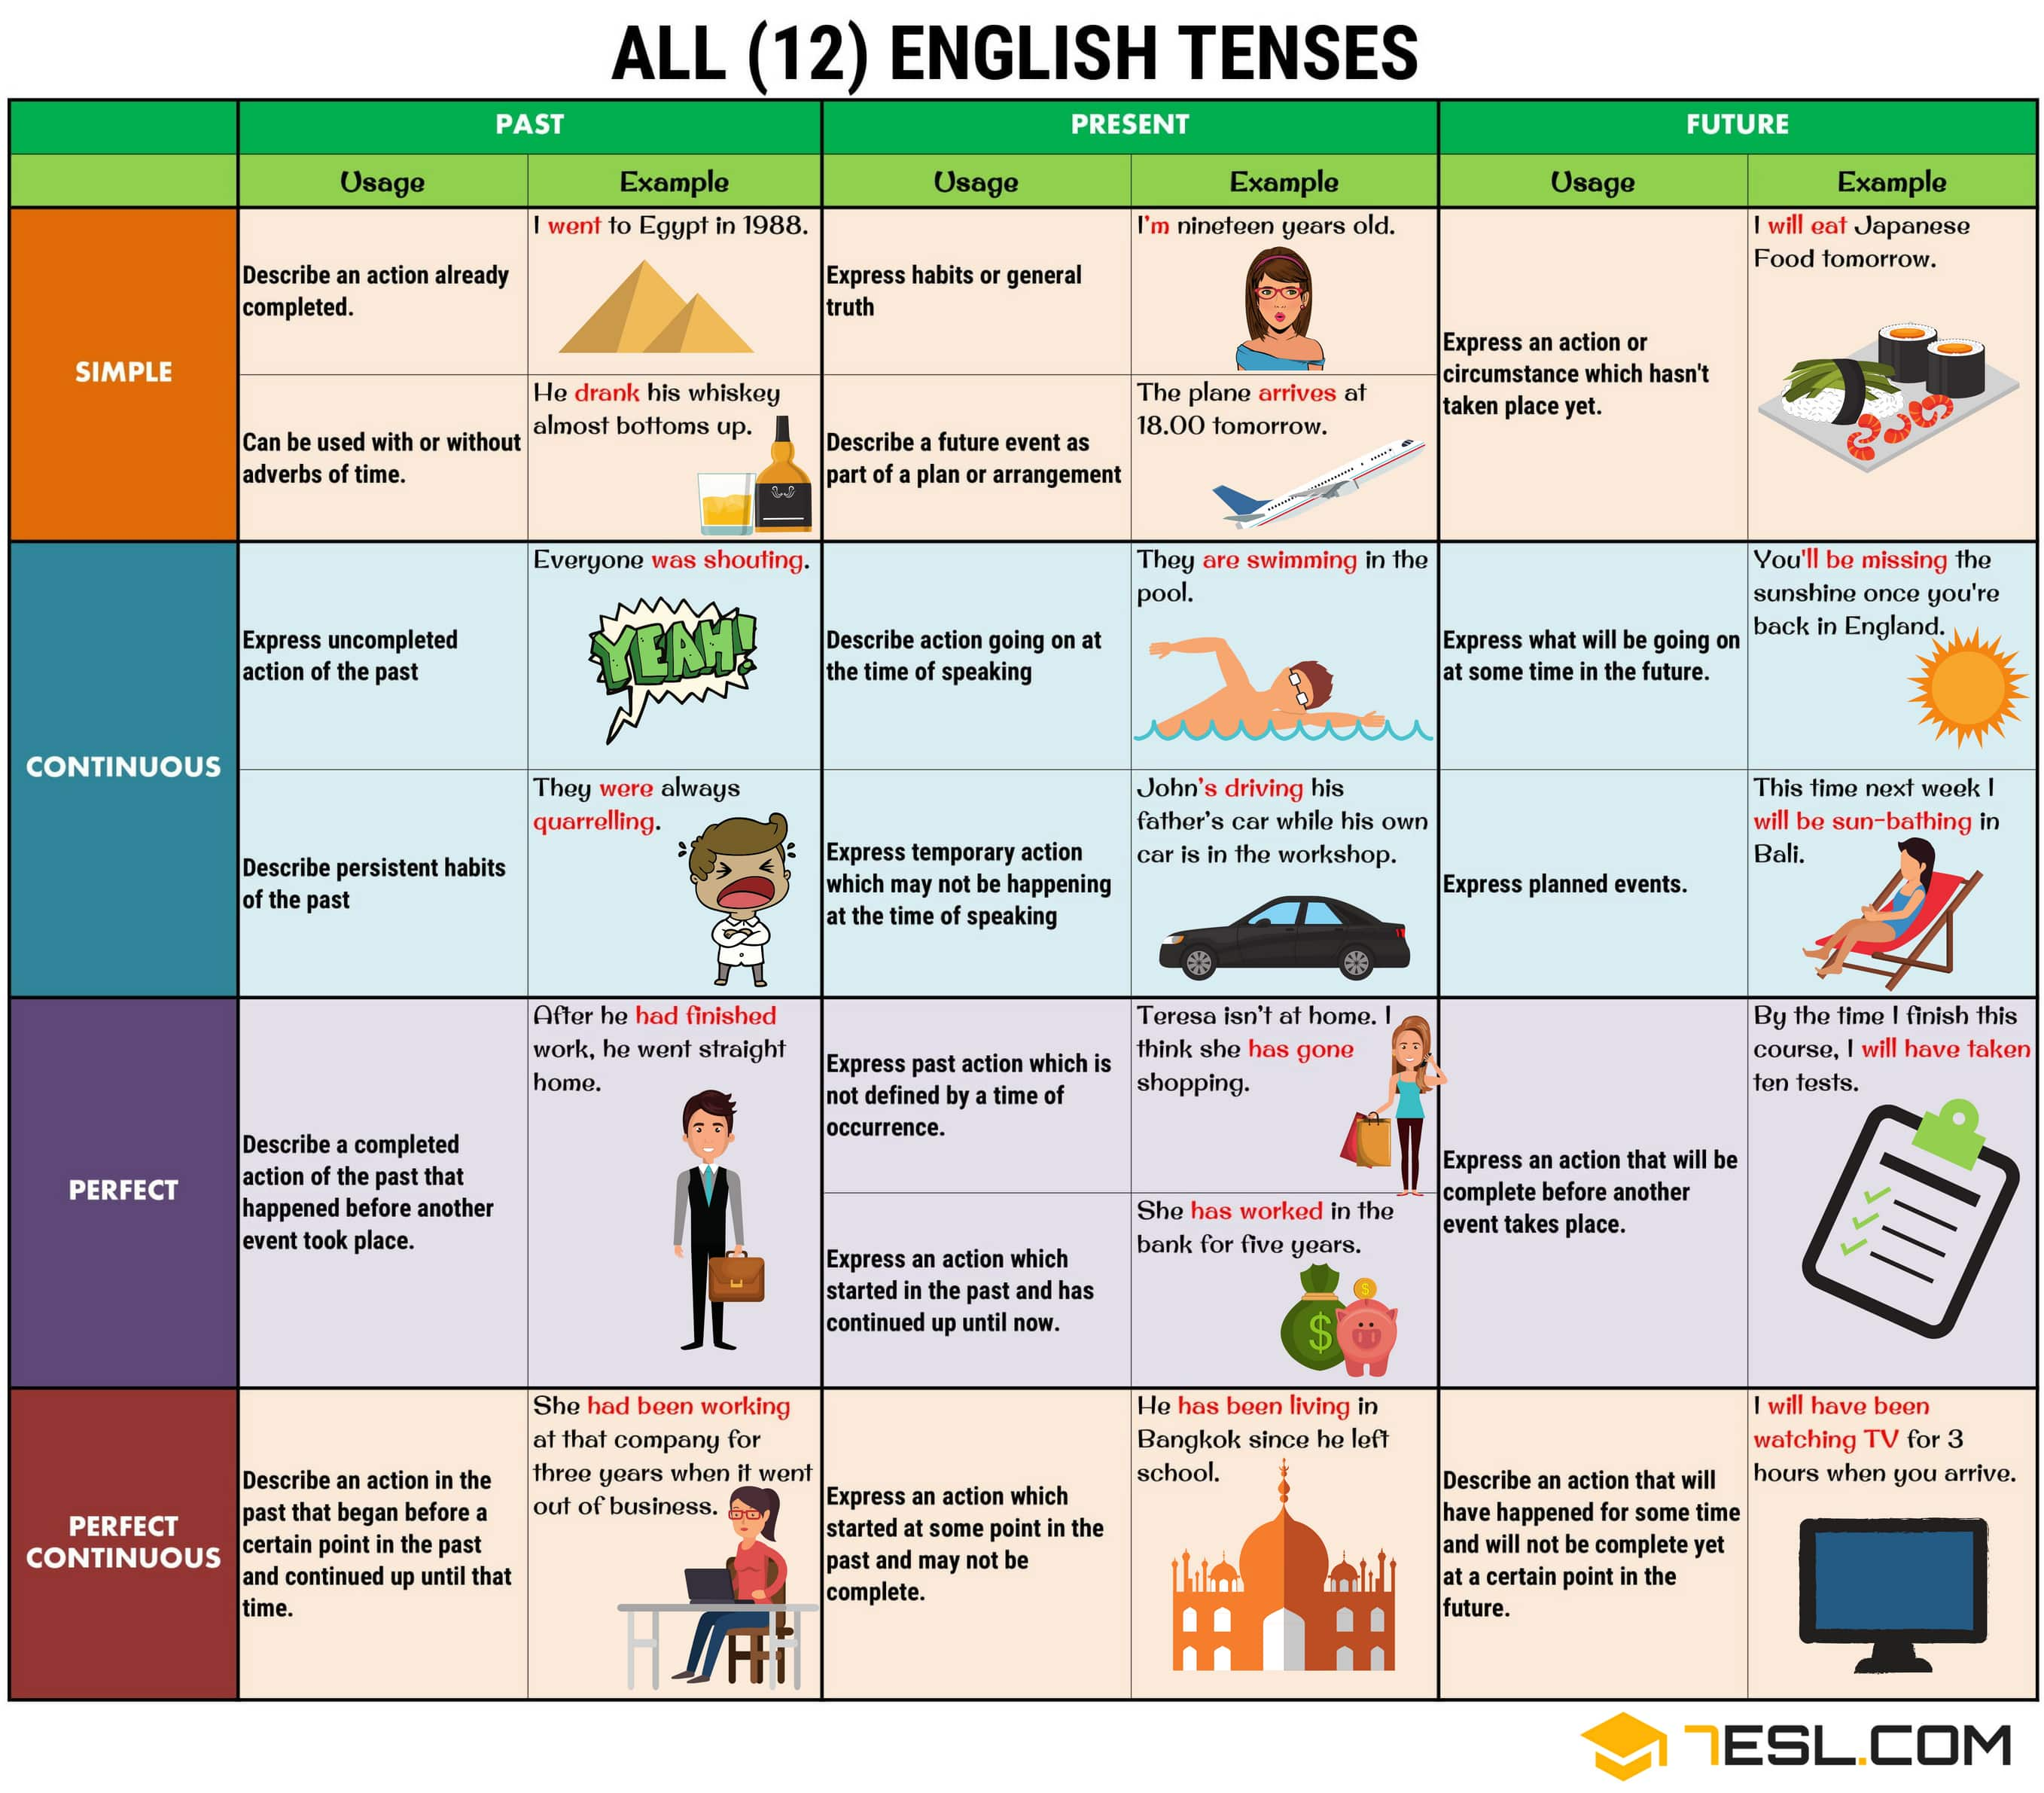
\includegraphics[width=\textwidth]{alltenses.jpg}
  \caption{\label{fig:alltense}英语全时态12种 (1)}
\end{figure}

\begin{figure}[p]
  \centering
  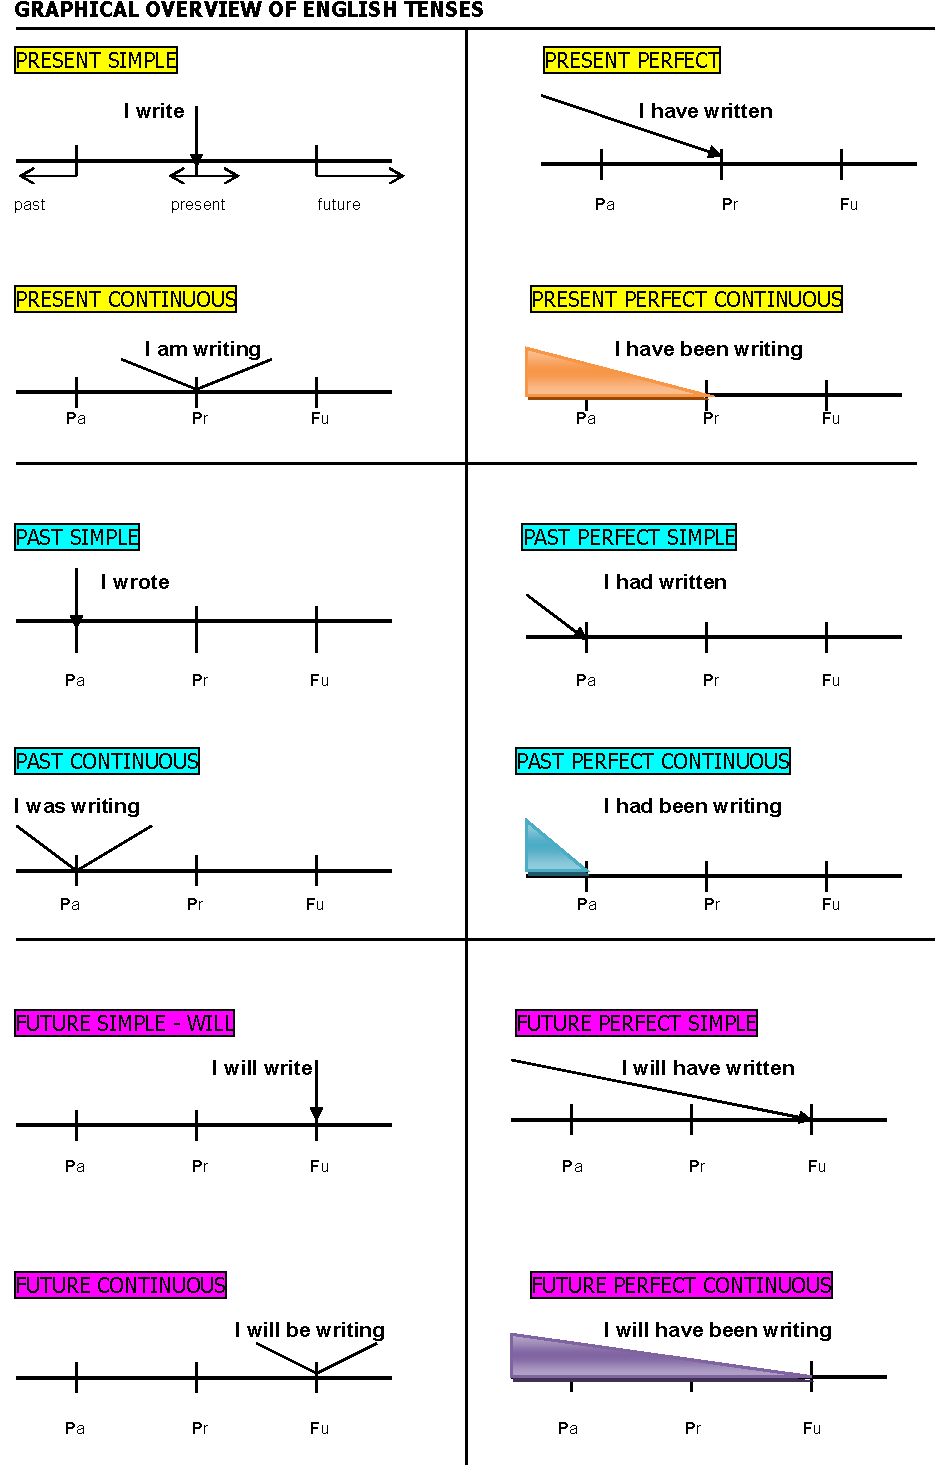
\includegraphics[height=1.1\textheight]{graphtenses.pdf}
  \caption{\label{fig:graphtense}英语全时态12种 (2)}
\end{figure}
\restoregeometry

\chapter{动词}

\section{时 (tense) 体 (aspect)}
\label{sec:tenseaspect}

\begin{description}
\item[时 (tense)] 在时间上定位一种情况,指示一个动作何时发生。
  \index{概念!时 tense}

  教学当中一般认为有过去时、现在时和将来时,见(\cref{fig:alltense} \cref{fig:graphtense})。但现代
  英语语法一般认为,英语只有两种语法编码的时态,\textbf{现在时}和\textbf{过去
    时}。至于为什么不包括将来时,可参考下一节。

\item[体 (aspect)] \index{概念!体 aspect}动作与时间相关联的表达方式,它关注动
  作的性质或状态,而不是时间。英语主要有四种体:\textbf{一般体}、\textbf{进行
    体}、\textbf{完成体}、\textbf{完成进行体}。
\end{description}

\section{不存在的将来时}

现代英语语法较多认为,英语没有将来时,因为它没有像许多其他语言那样的将来时变
化,也没有任何其他可以单独称为将来时的语法形式或形式组合。英语提供了各种将来
时的替代方式,以下例子均可表未来,且确定性大体上是依次递增。
\begin{description}
\item[will/shall/must/may 等情态助动词]
  \begin{itemize}
  \item Who do you think \unbf{will win} on Saturday?

  \item If you\unbf{'ll just wait} here for a moment, I\unbf{'ll see} if Mr
    Andrews is free.

    如果你要在这里等一会儿,我看看安德鲁斯先生是否有空。(委婉拒绝)
  \item What time shall we come and see you?

  \item We\unbf{'ll fly} at 30,000 feet.

    有机长临时决定的意思。

  \item We\unbf{'ll be flying} at 30,000 feet.

    will be doing,有“当然,必然”的意思,绝对会这样发展。
  \end{itemize}
\item[be to等半助动词] 确定性和情态助动词基本可一一相应,可见\cref{subsec:halfmodal}.
  \begin{itemize}
  \item There daughter is \unbf{to be married} soon.

  \item I\unbf{'m about to} read your book.
  \end{itemize}

\item[be going to + 不定式] 用于\textbf{某种意图的实现}或者\textbf{某种起因的后果}。
  \begin{itemize}
  \item I \unbf{am going to complain} if things don't improve.
  \item It's going to rain.

  \item She\unbf{'s going to have} a baby.
  \end{itemize}

\item[is/are doing 现在进行时] 根据决定、程序将发生的事。
  \begin{itemize}
  \item The match is starting at 2:30.

  \item I\unbf{'m leaving} the university in two year's time.
  \end{itemize}
\item[一般现在时] 用于 if, before, when 引导的从句中,把将要发生的动作当作确
  定的基点 。
  \begin{itemize}
  \item What will you say \unbf{if I marry} the boss?

  \item A: Are you going to the beach tomorrow?

    B: Yes, if the weather \unbf{is} good.
  \end{itemize}

  也可用于校历、时刻表,或过去现在将来基本不变等确定性最强的事件。
  \begin{itemize}
  \item School \unbf{finishes} on 21st March.

  \item The plain \unbf{takes off} at 20:30. [take off 为短语动词,起飞]

  \end{itemize}
\end{description}

此外,\textbf{在虚拟语气、假设从句中还可以用过去式表将来}……


\section{动词功能分类}

根据动词在动词短语中的功能,可分为三类:
\begin{description}
\item[全义动词 FULL VERBS] 又叫实义动词 lexical verbs,如play, grow, jump 等,只
  能用作主要动词。
\item[基本动词 PRIMARY VERBS] be, have, do,既可以作主要动词(注:系动词也是
  主要动词),也可作助动词。
\item[情态助动词 MODAL AUXILIARY VERB] may, might, will, would, can, could,
  shall, should, must,只可作为助动词,并且必须是\textbf{谓语部分第一个动词},
  它们能表达所谓情态 (MODALITY, 包括意愿、可能性、义务等)这一领域中的含义。

\end{description}

动词的 分词 participle 这个名称,也反映了这一形式既带有动词特征,又带有形容词
特征。

有些语法认知将动名词和现在分词分为两类,虽然他们屈折形式一致。另一些则认为动
名词只是现在分词一种表现形式。我们这里认可第二种,如此可说现在分词还可作为形
容词或名词使用。


\section{动词的第三人称单数及名词复数 -s }

\begin{enumerate}
\item 以清、浊咝声结尾的原形的-s 形式,结尾应是 es,读作  \doulos{/ɪz/},如以
  \doulos{/s z ʧ ʤ/} 等音。
\item 以清辅音结尾的原形后读作 \doulos{/s/},如 \doulos{/p t k f/} 等音。
\item 除咝声外,以浊音(包括元音)结尾的原形后,读作 \doulos{/z/}。
\item 以o结尾的一些单词要加 es,如go  \Rightarrow goes, echo  \Rightarrow echoes
\item 以 辅音 + -y 结尾的原形, 把 -y 变成 -i,后加 es : try \Rightarrow tries,carry  \Rightarrow carries。
\end{enumerate}

\subsection{规则动词的过去式和过去分词}

规则动词的过去式和过去分词:
\begin{enumerate}
\item 在以 \emph{t} 和 \emph{d} 结尾的原形后面读作 \doulos{/ɪd/}。 padded, patted
\item 在以浊音(包括元音)结尾的原形后面读作 \doulos{/d/}。buzzed, towed, called
\item 除 \emph{t} 外,在以清音结尾的原形后面读作 \doulos{/t/}。passed, packed
\item 以 辅音 + -y 结尾的原形, 把 -y 变成 -i,后加 ed:
  \begin{taskitem}(4)
    * try \Rightarrow tried
    * carry  \Rightarrow carried
  \end{taskitem}

\item 如果动词原形以单个辅音字母结尾,之前只有一个发元音的字母并且重读,那么它的现在分词和过去分词形式中要加双拼。
  \begin{taskitem}(2)
    * bar \Rightarrow barring \Rightarrow barred
    * beg \Rightarrow begging \Rightarrow begged
    * permit \Rightarrow permitting \Rightarrow permitted
    * patrol \Rightarrow patrolling \Rightarrow patrolled
  \end{taskitem}

\item 以 元音+c 结尾的动词原形,其现在分词和过去分词形式要加 k。如
  \begin{taskitem}(2)
    * panic \Rightarrow panicking \Rightarrow panicked
    * traffic \Rightarrow trafficking \Rightarrow trafficked
  \end{taskitem}

\item 如果原形以不发音的 -e 结尾,他的过去和现在分词形式,总是先删去 -e。
  \begin{taskitem}(2)
    * create \Rightarrow creating \Rightarrow created
    * type \Rightarrow typing \Rightarrow typed
  \end{taskitem}
\end{enumerate}

\subsection{不规则动词屈折变化}

请见\ccref{tab:irrverb} 。

\section{(半)情态助动词}

\begin{table}[htbp]
  \centering \small
  \begin{talltblr}[ caption = {情态助动词到主要动词的递差度表},
    label = {tab:auxverb},
    note{a} = {ought to用在肯定句中,否定和疑问句中则去掉to.}
    ]{
      width=\linewidth, colspec={X[-1,l]X[l]},
      rowspec={Q[t]Q[t]Q[t]}, rowsep=2pt, colsep=4pt,
      row{1} = {font=\bfseries},
    }
    \toprule
    动词类别 & 助动词或主要动词短语 \\ \midrule
    \textsf{主要情态助动词} &  may, might, will, would, can, could, shall, should, must \\
    \textsf{临界情态助动词} &  dare, need, ought to, used to \\
    \textsf{情态助动词习语} &  had better, would rather/sooner, be to, have got to等 \\
    \textsf{半助动词} &  have to, be about to, be able to, be allow to, be bound to, be going to, be likely to, be
    obliged to, be supposed to, be willing to 等 \\
    \textsf{系动词} &  appear to, happened to, seem to, get + -ed分词, keep + -ing分词等 \\
    {\textsf{主要动词+} \\\textsf{非限定性从句}} &  begin + -ing分词等 \\ \bottomrule
  \end{talltblr}%
\end{table}

\textbf{主要情态动词只可作助动词;而其他兼具情态助动词功能的动词还可作为主要
  动词使用}。因此要注意区分,如:
\begin{itemize}
\item \unbf{Need} we \unbf{escape}? We \unct{needn't escape}{V}. (need 作为
  情态助动词)

\item She \unbf{needs} \unbf{to practice}{A} and so \unbf{do} I. (need 作为主
  要动词)
\end{itemize}

有情态助动词功能的动词短语示例:
\begin{itemize}
\item No one \unct{dare tell}{V} the king this bad news.

\item We \unbf{ought to} give him another chance. \unbf{Ought} we have done it?

\item You\unbf{'d better} lock the door.

\item I\unbf{'d rather/sooner} live in the country \uline{than} in the city.
\item No one \unbf{is likely to} \unbf{be able to} recognize her.
\item \unbf{Has} he \unbf{to} answer the letter this week?
\end{itemize}

\section{动词短语}

\index{概念!动词短语 verb phrase}
\begin{description}
\item[动词短语] 句法中的谓语V(也被称作动词短语),由\textbf{1个主要动词和0--4个助动词}组
  成。
\end{description}


\begin{table}[htbp]
  \centering
  \begin{talltblr}[ caption = {动词短语},
    label = {tab:verbph},
    ]{
      width=\linewidth, colspec={r|l|l},
      rowsep=2pt, colsep=6pt,
      row{1} = {c, font=\bfseries},
    }
    \toprule
    助动词  & 主要动词 & 备注 \\ \midrule
     & sank & 一般过去时 \\
     was & sinking & 过去进行时 \\
     has been & sunk & 现在完成时,被动 \\
     must have been & sinking & 现在完成进行时 \\
     must have been being & sunk & 现在完成进行时,被动 \\
    \bottomrule
  \end{talltblr}%
\end{table}

过去传统语法将简单句化为\textbf{主部 (SUBJECT)}(和现代语法主语相同)
和\textbf{谓部 (PREDICATE)}(主语之后的部分)。而谓部又可分为\textbf{助动词和
  功能词}及\textbf{谓体 (PREDICATION)}(主要动词及之后部分)。\index{概念!谓
  部predicate}\index{概念!谓体 predication}如:
\begin{itemize}
\item \unct{The sun}{主部} \unct{was}{助动词和功能词} \unct{sinking in the
    west}{谓体}.

  was sinking in the west 为\textbf{谓部}。
\end{itemize}

\section{简化英语时态}

不必死记十几种英语时态(变成x * y 的笛卡尔积),只需要分别确定
时aspect和体tense,在将之加以组合即可(见\cref{sec:tenseaspect})。

\subsection{过去时间}

\begin{enumerate}
\item The U.S. \unbf{established} diplomatic relations with the P.R.C. \unbf{in 1979}.

  美国与中华人民共和国于 1979 年建交。

\item  The movable print \unbf{was introduced} to England in \unbf{1485}.

  活版印刷于 1485 年被引进英国。

\item I \unbf{was} visiting clients \unbf{the whole day yesterday} .

  昨天一整天我一直在拜访客户。

  yesterday表明整个事件发生在\textbf{过去},而the whole day突出\textbf{一直
    持续进行},现在分词可表阶段时间内的持续性,因此用过去进行时。
\end{enumerate}


\textbf{两种一般过去时之间}通常存在的是\textbf{时间先后顺序}关系;\textbf{过
  去进行时和一般过去时之间}则常是\textbf{时间内包关系 (TIME-INCLUSION)}:
\begin{itemize}
\item When we \unbf{arrived}, Jan \unbf{made} some fresh coffee.

  时间顺序,到达后煮咖啡。

\item When we \unbf{arrived}, Jan \unbf{was making} some fresh coffee.

  时间内包,到达时正在煮咖啡,到达的一瞬内包在煮咖啡期间。


\item I \unbf{was} watching TV \unbf{when I heard the doorbell} .

  听到门钤响的时候,我正在看电视。

  这个句子的时间状语“我听到门铃响的时候”,是指门铃响起来那一刹那,所以是很
  短的\textbf{一瞬间},英语中瞬息动词一般\textbf{用一般体},结合句子这里
  用\textbf{一般过去式} heared。而门铃响前和响时我\textbf{一直在看、持续在看}电
  视,所以主句用\textbf{过去进行时}。


\item  The witness \unbf{was being questioned} in court \unbf{when he had a heart attack} .

  证人心脏病突发时,他正在法庭上被质询。[同上]
\end{itemize}

\subsection{现在时间}

真理以及不变事实要用一般现在时表示。其实这也没什么好背的。因为,只有在以now为
中心的时间段可以大到涵盖过去与未来,才可以用来表示不变的真理。请看下面这些例
子:

\begin{itemize}
\item Huang \unbf{pitches} a fast ball. Li \unbf{swings}. It \unbf{looks} like a hit. The shortstop
  \unbf{fails} to stop it. It'\unbf{s} a double!

  黄投出快速球,李挥棒,好像是安打,游击手没有拦到球,是二垒安打!
\end{itemize}

播报运动比赛时,常会用到一连串的一般现在时。每个动作在当前一瞬间从发生到湮灭,
播报员所播报的一直是当前这一刻所发生的事情,所以用一般现在时。

其实,\textbf{一系列瞬息动作使用一般现在时,也为事件赋予了画面动感。}

\begin{itemize}
\item  Bush \unbf{is} the U.S. President.

  布什是美国总统。
\end{itemize}

布什是现任美国总统,可是几年前他不是,几年后他也可能不再是。这个句子的时间是
一个以now 为中心的括弧,所以用一般现在时。

\begin{itemize}
\item  All mothers \unbf{love} their children.

  天下的妈妈都爱自己的小孩。
\end{itemize}

天下的妈妈没有不爱小孩的。这是古今皆然,以后也不会改变,所以动词用一般现在时的love。

\begin{itemize}
\item  7-ELEVEN \unbf{is selling} big cokes at a discount \unbf{this month}.

  统一超市这个月大杯可乐打折。
\end{itemize}
this month是现在时;可乐打折,是正在持续中的活动,所以用 selling big
cokes。\textbf{以现在分词短语做补语来强调持续性}。

\begin{itemize}
\item According to the NASA survey, the ozone layer \unbf{is being depleted}.

  根据美国国家航空和航天局的研究,臭氧层正在被消耗中。

  当前事件 + 持续 + 被动,用现在进行时,且加以被动态。
\end{itemize}


\subsection{未来时间}

\begin{itemize}
\item  There \unbf{will be} a major election in \unbf{March}.

  三月将有一次大选。

  时间副词 in March是一个未来时间。未来的事情还没发生,尚未确定,所以要加一个
  助动词will 在前面,意思是“到时候会”。

\item Don't call me at six tomorrow. I'\unbf{ll still be sleeping}
  \unbf{then}.

  不要在明天六点时打电话给我。我那时还在睡觉。

  明天六点,将来;现在分词的词尾 \emph{-ing} 表示持续性,still be sleeping 一
  直在睡觉,强调自己不想被打扰的理由充足。

\item  The building \unbf{will be razed} \unbf{next month}.

  这房子下个月拆除。
\end{itemize}

时间副词 next month 是一个未来时间的括弧,所以动词用未来一般体:will be。后面
的razed(被拆除)是过去分词,当形容词补语看待,形容主语“房子”。

\subsection{完成体}

从功能上来看,\textbf{一般体是交代动作发生的具体时间点(段);而完成体并不对
  动作发生的时间点(段)作明确交代,其只表示在一个更为宽泛的时间段
  内“曾经”、“做过”的意思;且隐含或明显强调截止日期。}

\begin{itemize}
\item  I\unbf{'m} sure I \unbf{have seen} this face somewhere.

  我肯定曾经见过这张脸。
\end{itemize}
主要从句 I'm sure 的动词 am表示是现在时间,除此之外,没有时间副词交
代“看到”这张脸的具体时间,只知道一定有见过。这就是现在时间完成式的条件,所
以用have seen(看过)。

\begin{itemize}
\item We \unbf{have been working} overtime \unbf{for a week} to fill your order.

  我们连续加班一个星期赶出你订的货。
\end{itemize}

时间副词for a week是“\textbf{到现在为止}已经有……了”,强调了\textbf{截止时
  间}并且截止时间是\textbf{现在},要用\textbf{现在完成时}“已经”来配合。

除此之外,该句强调在一个大的时间段内\textbf{一直在进行}的工作,所以要
用\textbf{进行时}。


\begin{itemize}
\item  The house \unbf{has been redecorated} twice \unbf{since they moved in}.

  打从他们搬来算起,这栋房子已经被装修过两次了。
\end{itemize}

since they moved in(打从他们搬来算起),截止时间是当前,所以主句用完成体。
且装修要用被动态。


如果没有特别交代的话,一般说“有……过”就是“到现在有……过”,所以都是现在
完成式。用过去完成时时则要有一个过去的截止时间,在那之前就“有……过”。

\begin{itemize}
\item  Many soldiers \unbf{had died} from pneumonia \unbf{before the discovery of penicillin}.

  发现盘尼西林以前,已经有很多士兵死于肺炎。
\end{itemize}

盘尼西林在 1928 年发现,before the discovery of penicillin,表明这是一
个 \textbf{以 1928 年为截止时间的时间段内,所以要用过去时间的完成式 had
  died。}

\begin{itemize}
\item  I \unbf{had been smoking} three packs of cigarettes a day \unbf{before I decided to quit}.

  我决定戒烟之前,每天要抽三包烟。
\end{itemize}

before I decided是“在我决定之前”的一大段时间,以 decided为\textbf{截止时间}。
这就得用过去完成时 had been。smoking three packs中的 \textbf{-ing表示持续性,
  也就是每天都要抽三包烟,而且是“一直如此”,}用来形容主语“我”。


\begin{itemize}
\item  Japan \unbf{had not been defeated} yet \unbf{by the time Germany surrendered} unconditionally.

  到德国无条件投降为止,日本尚未被打败。
\end{itemize}


未来时间的完成式,只是把截止时间后移到未来的一个点。观念上与现在、过去时间的
完成式完全一样。在写法上,因为是未来时间,所以动词前面加一个will 就可以了。请
看例句:

\begin{itemize}
\item  \unbf{Next April}, I \unbf{will have worked} here \unbf{for 20 years}.

  到四月,我在这里就工作 20 年了。
\end{itemize}

next April 结合 for 20 years,表明截止到四月、为期二十年的时间段,所以要用完
成式。动词前面加上will,表示到现在还没有,要到四月才“会”做满 20年,也就是未
来时间的完成式。

\begin{itemize}
\item  Come back \unbf{at 5:00}. Your car \unbf{will have been fixed} \unbf{by then}.

  五点再来吧!到时候你的车一定已经修好了。
\end{itemize}

你去修车厂拿车子,老板叫你五点再来。他的意思不是五点才要修你的车,而是说五点
以前就一定先修好了,等你来拿。真正修好的时间可能是四点,也可能是三点也说不一
定,反正不超过五点。这就是完成式的时间段且\textbf{截止时间在未来},所以用未来
完成时,车辆用被动态表示被修理厂工人修好,所以用will have been fixed。

\begin{itemize}
\item \unbf{In two more minutes}, she \unbf{will have been talking} on the
  phone \unbf{for three hours}!

  再过两分钟,她就一直打了足足三小时的电话了!
\end{itemize}

In + 数词 + 时间,表示从现在算起,多长时间内。该句截止时间为
在\textbf{将来}的2分钟后。用将来完成时。be talking 表示持续在做某事,所以该句
用将来完成进行时。

\section{Test}

\subsection{练习一}

\textbf{请选出最适当的答案填入空格内,以使句子完整。}

\begin{enumerate}
\item So far we \ttu nothing from him.
  \begin{tasks}(2)
    \task have been heard
    \task did not hear
    \task have heard
    \task have not heard
  \end{tasks}


\item At present a new road \ttu in that part of the city.
  \begin{tasks}(2)
    \task is building
    \task will be built
    \task will have built
    \task is being built
  \end{tasks}

\item Our city \ttu a great deal. It doesn't resemble the one of three years ago.
  \begin{tasks}(2)
    \task changes
    \task has changed
    \task is changing
    \task will change
  \end{tasks}

\item When Anna phoned me I had just finished my work and \ttu to take a bath.
  \begin{tasks}(2)
    \task was starting
    \task have started
    \task starting
    \task will start
  \end{tasks}

\item There \ttu some very bad storms recently.
  \begin{tasks}(4)
    \task is
    \task are
    \task have been
    \task have
  \end{tasks}

\item  The future price of this stock \ttu by several factors.
  \begin{tasks}
    \task is going to determine
    \task will determine
    \task will be determining
    \task will be determined
  \end{tasks}

\item The camera was invented in the 19th century. At that time, most photographers \ttu professionals.
  \begin{tasks}(2)
    \task are
    \task were
    \task have been
    \task had been
  \end{tasks}

\item The whole area was flooded because it \ttu for weeks.
  \begin{tasks}(2)
    \task rains
    \task has rained
    \task had been raining
    \task was raining
  \end{tasks}

\item By next Sunday you \ttu with us for three months.
  \begin{tasks}(2)
    \task will have stayed
    \task will stay
    \task shall stay
    \task have stayed
  \end{tasks}

\item \textbf{We could smell that someone \ttu a cigar.}
  \begin{tasks}(2)
    \task would be smoking
    \task was smoked
    \task had been smoking
    \task would be smoked
  \end{tasks}

\end{enumerate}

\subsection{练习二}

\textbf{请把括弧中的动词以适当的时态填入空格内,以使对话内容完整。}

item Boy: Do you want to go and see \textit{Gone with the Wind} with me tonight?

Girl: No! I \ttu (1. see) it.

Boy: Oh, really? When did you see it?

Girl: I \ttu (2. go) to see it the first day it was on-last Monday.

Boy: To tell you the truth, I have seen it too. In fact, I \ttu (3. see)it before you did.

Girl: That's impossible. I told you I saw it the first day it was on.

Boy: But it's the truth! I \ttu (4. see) it seven or eight years ago, the
last time that old picture \ttu (5. come) in town.


Girl: In that case, why did you ask me to go in the first place? Boy: Well,
I just \ttu (6. want) to go out with you tonight. Since you have seen the
picture, will you go to the baseball game with me instead?

Girl: I \ttu (7. guess) I will, if Father says Okay. But you will have to
pick me up at my place.

Boy: Great! I \ttu (8. see) you at 5:30 then. I'll bring my car.

Girl: But why 5:30? Why not seven o'clock?

Boy: Because the game \ttu (9. start) by then. These evening games \ttu (10.
begin) at 6:30, you know. Don't forget now, 5:30 at your place!

\section{Answer}

\subsection{练习一答案}

\begin{enumerate}
\item (C) so far(到目前为止)应用现在完成时,故排除过去式的 B。主语是 we,表示“我们听到”时应用主动态,故排除被动的 A。因空格后已有否定的 nothing,所以不选表示重复否定的 D。

\item (D) at present 表“现在”,应用现在时,故排除未来式的 B 和 C。主语 road 与
  动词 build 配合,应用被动态表示“被建造”,故排除主动的 A。答案 D 表示“现
  在正在被建造中”。

\item (B) “现在它和三年前已大不相同”,可以看出,空格那个 change 要表示的是从三
  年前到现在的改变,因此选择现在完成时 B。A 和 C 其实也没错,表示它“经常在
  变”,不过这两个答案与题目第二句的呼应不及 B 密切。D 的将来时则和题目第二句
  有较大的冲突。

\item (A) 从 when Anna phoned me 以及 I had just finished 可看出时间在过去,因此
  表示现在时间的 B 和未来时间的 D 都可排除。又,空格前面有对等连接词 and,要
  求对称。在 A 和 C 之中只有 A 是动词短语,可以和前面的动词短语 had just
  finished 对称。

\item (C) recently 表示“不久前到现在”,应用现在完成时。表示“有”的观念应
  用 \textbf{There is/are 的句型,其现在完成时即是 have been(主语 storms 是
  复数)}。

\item (D) 从 future price(未来价格)可看出时间在将来。主语 price 与动
  词 determine 配合应用被动态,这点从空格后面的 by several factors 亦可看出。
  唯一正确的被动态是 D。

\item (B) 从 at that time 可看出时间在过去(19 世纪)。因明确表示出那一段时
  间,句子前后时间一致,且前面一句用的是was,所以后句应该也应用一般过去时,故选 B。

\item (C) 从主要从句 was flooded 可看出,淹水是过去时间,而造成淹水的原因
  “下雨”,只能在淹水之前发生,表示一大段时间内的持续,所以该用过去完成进行
  时。

\item (A) next Sunday 表示未来时间,故排除现在时间的 D。然后介词 by 表示“到……为止”,应用完成式,因而排除一般体的 B 和 C。

\item (C) 主语 someone 和动词 smoke(有人抽雪茄)配合应用主动态,故可排除被动
  的 B 和 D。而 A 的 would be smoking 表示“将抽未抽”,如此则和 we could
  smell(已闻得到)有冲突,故选过去完成时的 C,表示在那之前已有人在抽,才会留
  下味道。

\end{enumerate}

\subsection{练习二答案}

\begin{enumerate}
\item have seen 看过,而不说何时看的,应用现在完成时。

\item went 既说出看的时间(last Monday),应用一般体。

\item had seen 时间是 before you did,只知在过去时间 you did 之前,未明言在何时,
  应用过去完成时。如果用 saw 也不算错,因为在 I saw 和 you did 之间有 before
  相连,清楚交待两个动作的先后,不必倚赖过去完成时来交待。

\item saw 因交待了“七八年前”,应用一般体。用 had seen 也不算错,这样的语气
  是“我看得比你早”,至于“七八年前看的”这点则在语气上不予强调。

\item came 因有 the last time 标出时间,应用一般体。

\item wanted 因为是回应 Why did you \ldots{} ?

\item guess 这是这位小姐说话时的猜想,时间就是 now,应用现在式。

\item will see 因为说出 at 5:30 的未来时间。

\item will have started 因为时间是 by then,也就是“到了那个时候”,老早开打了。
  没说几点开打,总之在那之前,这就是完成式。也可用 would have
  started,用 would 不是表示过去时间,而是表示非事实的假设,成为:“如果真的
  拖到七点才去的话,那就看不成了,非早点去不可!”这样的口吻。

\item begin 因为 \textbf{these} evening games 不只说今晚这场,而是“所有的晚场比赛都是”,
  也就是说包括今天的这一阵子都是如此,就得用一般现在时。
\end{enumerate}

\chapter{不定式}

\section{带to与不带to的不定式}

不带to的不定式中第一个动词用动词原形,因此很多人不知道不带to的不定式,只知道
动词原形。

虽然可认为不带to不定式是动词原形的一种应用。但我觉得,最好还是将动词原形与不
带to的不定式区做下区分为好,因为\textbf{不带to不定式之前有助动词或类似动词},
而前面的(类)助动词有“体”aspect的变化;以及“不定式”可以表示词性多变。

\begin{description}
\item[动词原形] 动词的基本形式,可以通俗认为只用在\textbf{祈使句}。\textbf{既没有时态
  的标记,也没有体的变化。}
  \begin{itemize}
  \item \unbf{Come} here.

  \item Let us \unbf{party}.
  \end{itemize}

\item[不带to的不定式] 用在\textbf{否定助动词},\textbf{情态助动词}(can,
  may, could等),\textbf{感官动词}(see, hear, feel等),\textbf{使役动
    词}(let, make, have等)后面,采用动词原形形式。

  let是个小品词,有一点词性模糊。

\item[带to的不定式] to + 动词原形。可以\textbf{将其中的to理解为情态助动词功
    能},并常表示\textbf{有不确定性}。
\end{description}

不同于原形,两种不定式都\textbf{没有时态的标记,但有体aspect的变
  化。} 如should/to \unbf{write}, should/to \unbf{be} writing, should/to
\unbf{have} written, should/to \unbf{have} been writing, didn't \unbf{do}.

\section{to与助动词的共同点}

要了解不定式与助动词之间的关系,不妨先看一个例子:

\begin{itemize}
\item  I am glad \unbf{to know you}.

  很高兴能认识你。
\end{itemize}

这是一句简单的会话用语,读者应该都能脱口而出。可是如果追问下去:“为什么用不
定词to know you?”“为什么不能用动名词 knowing you?”恐怕许多读者就答不上来
了。(请不要回答“我背过”,或者“这是惯用法”、“这是短语”;语法要求理解,
不能打迷糊仗。)其实,只要了解不定式与助动词之间的关系,就可以了解这个不定式
是来自助动词的变化。怎么说呢?我们来看看这个例句还原成原状的样子:

\begin{itemize}
\item  I am glad \unbf{because/that I can know you}.
\end{itemize}

这句话可以进一步改写为下面这个类似的句子:

\begin{itemize}
\item  I am glad \unbf{because/that I am able to know you}.
\end{itemize}

由连接词 because 所引导的状语从句中,主语 I和前面主要从句的主语相同,是重复的
元素。动词 am 是个空的 be动词,没有意义。因此这两个元素(I am)都可以省略。可
是,状语从句中省略主语与动词之后,已经不成一个完整的从句结构了。如此一来,连
接词because 也就没有必要存在。剩下的不定式 to know 本身就带有 able to的暗示,
所以就变成:

\begin{itemize}
\item  I am glad \unbf{to know you}.
\end{itemize}

翻译成“很高兴能认识你”,是因为这个 to know 就是 able to know,也就是can
know 的变化。

从这个例子可以看出,不定式与助动词的关系极为密切,我们可以利用这层关系来练习
判断不定式的用法。首先,我们来观察一下不定式与助动词之间有什么共同点。

\subsection{后面都要用动词原形}

\begin{itemize}
\item I \unbf{will go}.

  我要走了。
\item I \unbf{want to go}.

  我想去。
\end{itemize}

\subsection{都有“不确定”的语气}

\begin{itemize}
\item He \unbf{is} right.

  他是对的。
\item He \unbf{may be} right.

  他可能是对的。
\item He seems \unbf{to be} right.

  他好像是对的。
\end{itemize}

第一句 He is right是确定的语气,把“他是对的”当作事实来叙述。一旦加上助动
词 may之后,就成了不确定的语气。所以第二句 He may be right只是一个推测,不是
事实叙述。第三句He seems to be right也是推测,不是事实叙述。这种\textbf{不确
  定语气}是to与助动词之间一个很重要的共同点,可以用来判断何时该用带to不定式。

\subsection{都要用完成式来表达相对的过去时间}

助动词与不定式中的to本身都无法完整表达过去时间。如果你听到“哗啦哗啦”的声音
从外面传来,可以说:
\begin{itemize}
\item It \unbf{must be} raining now.

  一定下雨了。
\end{itemize}

如果看到天上乌云密布,一副山雨欲来的样子,也可以说:
\begin{itemize}
\item It \unbf{may} rain \unbf{any minute}.

  随时都可能下雨。
\item It \unbf{might} even snow.

  说不定还会下雪。
\end{itemize}

这几个例子中,第一句的助动词 must 没有过去式的拼法。至于第二句、第三句的may
和might,咋看之下好像有现在式和过去式的区别。可是用在猜测语气中并不是如
此。It may rain any minute 是未来时态,It might even snow同样也是未来时态,这
时的 might 并不是 may的过去式,只表示比较保留、比较没有把握的猜测语气。所以,
不论像 must这类只有一种拼法的助动词还是像 may,might这类有两种拼法的助动词,
都只能用来猜测现在或未来时间的事情,\textbf{助动词本身缺乏表达过去时间的能力}。

如果你早上起来看到地上湿湿的,于是说:

\begin{itemize}
\item  It \unbf{must have rained} last night.

  昨晚一定下过雨。
\end{itemize}

\textbf{在猜测过去的事情时,助动词不论是 must、may 还是might,都只能表示语气强弱的
  差别,无法表达过去。}助动词后面要接动词原形,也不能用过去式,所以别无选择,
只好用\textbf{完成式}来表示过去,也就是must have rained 这种形态。就这点来看,不定
词仍然与助动词相同。

\begin{itemize}
\item  It \unbf{seems to have rained} last night.

  昨晚好像下过雨。
\end{itemize}

这个句子的动词 seems是现在式,表示“现在看起来”、“现在的推测”。可是推测的
事情是昨天晚上的事,是过去的时间,所以“下雨”应该是过去式,但是\textbf{to与助动
  词一样,本身缺乏表达过去的能力},后面都要接动词原形,也不能用过去式,所以
只能用\textbf{完成式}来表示过去,变成to have rained。这又是不定式和助动词的一个共同
点。

\subsection{所有重要的情态助动词,都可以改写为不定式}
\label{subsec:halfmodal}

请观察以下的对照:
\begin{table}[htbp!]
  \centering
  \begin{talltblr}[ caption = {情态助动词可改写为不定式(半助动词)},
    label = {tab:modalinf},
    ]{
      width=\linewidth, colspec={ccc},
      rowsep=2pt, colsep=4pt,
      row{1} = {c, font=\bfseries},
    }
  \toprule
  情态助动词 & 不定式\\\midrule
  must & have to \\
  should & ought to \\
  will/would & be going to \\
  can/could & be able to \\
  may/might & be likely/allowed  to \\
  \ul{be (just) going to} & be about to \\
  \bottomrule
  \end{talltblr}%
\end{table}

从以上来看,\textbf{不定式中的to与助动词其实是同一种东西的相互变化}。

凡是不定式出现的地方,都可以看成是另外一个从句的省略:\textbf{把主语省略,助
  动词改为相应不定式}。

\section{不定式与动名词的区分}

传统语法所称的\textbf{动状词(Verbals)},包括现在分词(Ving)、过去分词
(Ven)、动名词(Ving)与不定式(to V)等等。其中\textbf{现在分词、过去分词有
  时还可以是形容词类},\textbf{不定式}则是“不一定什么词类”:它可以
当\textbf{名词、形容词、副词}使用。这就产生了一些混淆点。比如说,动词后面的宾
语位置,必须用名词类。可是动名词和不定式都可以当做名词使用(分词只能当形容词,
可以不必考虑),到底应如何区分?这就要借助我们刚才的观察了。现在来看看几个具有
代表性的动词:

\begin{description}

\item[plan]
  \begin{itemize}
  \item  \unct{They}{S} \unct{plan}{V} \unct{to marry next month}{O}.

    他们计划下个月结婚。
  \end{itemize}

  这个句子的 to marry next month 是 plan的\textbf{宾语},必须用名词类。那么为
  什么用不定词 to marry,而不用动名词 marrying呢?因为 to marry next month 就
  是 (that) they will marry next month的变化。marry 是计划中的事情,下个月才
  要发生,是\textbf{将来时}。再把 they will marry 改成 they are to marry。这
  时候,如果把重复的主语 they 和空的 be动词 are 省略掉,就成了不定式 to
  marry。

\item[avoid]

  \begin{itemize}
  \item  \unct{I}{S} \unct{avoid}{V} \unct{making the same mistake twice}{O}.

    我避免犯同样的错误。
  \end{itemize}

  这里用 making 比用 to make 恰当,因为 to make 是 will make的省略,既然
  是“\textbf{避免}”,后面又用 will make(将要做),意思就变得不清楚了:

  \begin{itemize}
  \item \unct{I}{S} \unct{avoid}{V} \unct{something}{O}.
  \item  I will make the same mistake twice.
  \end{itemize}

  \textbf{四种动状词中,只有动名词和不定词可以做名词类使用},也就是说:只有这
  两个可以当avoid 的宾语。如果用不定词 to make,则带有 I will
  make这种\textbf{将来时或者不确定}的涵意,与 avoid这种具有\textbf{否定}意思
  的动词并不适合并列,所以只剩下动名词 making是唯一的选择了。


\item[dislike]
  \begin{itemize}
  \item \unct{I}{S} \unct{dislike}{V} \unct{standing in long lines}{O}.

    我讨厌排队。
  \end{itemize}

  动词\textbf{dislike(不喜欢)本身是否定的,后面就不适合接 I will stand in
    long lines(愿意排队)}。而且 dislike 不像 hate,它\textbf{没有“必
    须”(have to)的暗示}。所以 dislike 的后面接 to stand就不适合了。既然不
  能用不定式,就只剩下动名词可以用了,所以要说 I dislike standing \ldots。
\end{description}

\textbf{后面通常接动名词的还有 avoid, consider, delay, deny, enjoy,
  escape, finish, give, up, imagine, involve, mention, mind, miss, postpone,
  practice, resist, risk, suggest等。}
\todo[inline]{更新后面只接动名词或不定式的动词。}


\section{接不定式和 -ing 从句皆可的动词}

有些动词后面可接不定式,也可接 -ing分句,但其语义上往往有差别。了解这方面内
容可对不定式或 -ing从句加深理解。

\begin{description}
\item[remember doing] 记得\textbf{过去发生过}的事,可有\textbf{持续性}。
  \begin{itemize}
  \item I still \unbf{remember buying} my first bicycle. [remember that I had bought]
  \end{itemize}

\item[remember to do] 记得\textbf{将来应该做}的事,有\textbf{不确定性}(可能最终也未做此事)。
  \begin{itemize}
  \item You must \unbf{remember to fetch} Mr Lewis from the station tomorrow. [remember
    that you are to]
  \end{itemize}

\item[forget doing] 忘了\textbf{过去发生过}的事,可有\textbf{持续性}。
  \begin{itemize}
  \item I\textbf{'ll} never \unbf{forget meeting} the Queen \textbf{in 1988}.
  \end{itemize}

\item[forget to do] 忘做\textbf{应该做}的事,有\textbf{不确定性}(未发生)。
  \begin{itemize}
  \item I \unbf{forgot to buy} the soap.
  \end{itemize}


\item[go on doing] \textbf{持续}做\textbf{过去已经在做}的某事,可有\textbf{持续性}。
  \begin{itemize}
  \item She \unbf{went on talking} about her illness until midnight.
  \end{itemize}

\item[go on to do] (停止其他动作,)\textbf{继续}做某事,\textbf{动作非持续,有转折。}

  \begin{itemize}
  \item She stopped talking about that and \unbf{went on to do} her job.
  \end{itemize}

\item[regret dong] 后悔、遗憾\textbf{做过某事},有\textbf{持续性}。

  \begin{itemize}
  \item I \unbf{regret leaving} school at 16 –-- a big mistake. [ I regret \unbf{that I
      left} school at 16]
  \end{itemize}

\item[regret to do] 为\textbf{不得已发生的事情}感到抱歉、遗憾,并非真正后悔。

  \begin{itemize}
  \item We \unbf{regret to say} that we are unable to help you. [regret \unbf{that we
      should say} that]
  \end{itemize}

\item[see, watch, hear等] 可以接 doing(\textbf{正在发生,还未结束,持续性});
  也可接不带to的不定式(\textbf{事情已完成})。
  \begin{itemize}
  \item I looked out of the window and saw Emily \unbf{crossing} the road.
  \item I saw Emily \unbf{cross} the road and \unbf{disappear} into the bank.
  \end{itemize}


\item[try] 接doing或不定式均可,尝试做困难的事。但try doing有期待某一种结果的意
  思。
  \begin{itemize}
  \item I \unbf{tried sending} her flowers, but she still wouldn't speak to me.
  \item John isn't here. \unbf{Try phoning} his mobile.
  \end{itemize}

\item[like, love, hate, prefer] 接doing或不定式均可。不定式可以有\textbf{尚未发生},或
  \textbf{不得不}的意思。
  \begin{itemize}
  \item I \unbf{hate to tell} you this, but we're going to miss the train.

  \item ``Can I give you a lift?'' ``No thanks, I'd \unbf{prefer to} walk.''

    give you a lift: 载你一程
  \end{itemize}

\item[begin, start, continue] 接doing或不定式均可。

\item[stop] 停止\textbf{正在做}的事情,用doing;\textbf{停下其他事情做某事},
  用不定式。
  \begin{itemize}
  \item We \unbf{stopped taking} pictures.

    We were no longer taking pictures.

  \item We \unbf{stopped to} take pictures.

    We stopped what we were doing so that we could start taking pictures.
  \end{itemize}

\item[advice, allow, permit, forbid] 不接宾语时,用doing (SVO, -ing 从句做宾语);接宾语
  时,一般接不定式 (SVOO, to- 不定式从句做直接宾语)。
  \begin{itemize}
  \item I wouldn't \unbf{advise taking} the car – there's nowhere to park.
  \item I wouldn't \unbf{advise you to take} the car …
  \item We don't \unbf{allow/permit smoking} in the lecture room.
  \item We don't \unbf{allow/permit people to smoke} in the lecture room.
  \end{itemize}
\end{description}

另外,go/get/walk/point/visit/down/be used 等位置\textbf{副词后接的to为介词,
  不是不定式标记to,如后接动词,需用 -ing}。

\section{使役动词与不带to的不定式}

了解不定式是什么,就能了解\textbf{使役动词的后面为什么要接不带to的不定式}。我们先来比较一下
使役动词和一般动词有什么差别。

\begin{itemize}
\item \unct{The little girl}{S} \unct{asked}{V} \unct{her mother}{O} \unct{to
    come to the PTA meeting}{C}.

  小女孩邀请妈妈来开母姊会。
\end{itemize}

这个句子可以改写为:

\begin{itemize}
\item  \unct{The little girl}{S} \unct{asked}{V} \unct{if her mother would come to the PTA meeting}{O}.
\end{itemize}

ask是普通动词,邀请人参加,但别人愿不愿意是不确定的,所以会牵涉到语气助动
词would come,这就会变成不定式 to come。

使役动词与普通动词的差别就在于它有\textbf{强制性},它的结果是确定的、无从选择的。因为
这种确定性的语气,\textbf{排除了助动词、to存在的空间},因而也就不能用带to的不定式。

\begin{itemize}
\item  \unct{The teacher}{S} \unct{made}{V} \unct{the little girl}{O} \unct{stay behind}{C}.

  老师叫小女孩留下来。
\end{itemize}

如果老师客客气气地问:Will you stay behind? 就会成为下面这句叙述:
\begin{itemize}
\item \unct{The teacher}{S} \unct{asked}{V} \unct{the little girl}{O} \unct{to stay behind}{C}.
\end{itemize}
这个小女孩有选择的自由,她愿不愿意留下来这点还不确定,所以会有助动词,也就会
变成不定式。可是如果老师是命令她留下来,没有选择的余地,那么老师说的就
是:Stay behind! 请注意:\textbf{祈使句的动词原形},表示的就是强迫的语气。它
要求结果是确定的,已经没有助动词或to存在的空间,这时候就不会变成不定式,而是
动词原形。像let、have、make等\textbf{使役动词},后面是接\textbf{不带to的不定
  式},就是因为这种强迫性的命令语气,使它的结果不具有不确定性,因而不能用to。

当然\textbf{这并不表示使役动词的后面只能用不带to的不定式},例如:
\begin{itemize}
\item \unct{John}{S} \unct{had}{V} \unct{his car}{O} \unct{painted over}{C}.

  约翰把车子让人重新漆过了。
\end{itemize}
\textbf{had +宾语 + 过去分词表示被动态。}

\section{感官动词与不带to的不定式}

感官动词的后面接不带to的不定式的道理,与使役动词是相同的:因为to的不确定性不
适合这个上下文。

\begin{itemize}
\item \unct{I}{S} \unct{heard}{V} \unct{her}{O} \unct{playing the violin}{C}.

  我听见她在拉小提琴。
\end{itemize}

所谓\textbf{感官动词},就是 see、hear、watch等等。它们后面\textbf{不适合
  用to},是因为to是助动词的变化,有不确定的语气。如果说to play the violin,那
就表示 she would play the violin(她想要或将要去拉小提琴),那么你听得到吗?
所以感官动词这种“听到、看到”的字眼,只能\textbf{配合确实发生的事使用},而不
能和带有“不确定、未发生”涵意的不定式连用。

那么,感官动词可否与\textbf{现在分词}一起使用呢?当然,如果她正在拉琴被我听到,
那么用现在分词playing 来表示\textbf{持续性}是最好的。可是:
\begin{itemize}
\item  I \unbf{heard her cry out} in pain.

  我听到她痛得大叫一声。
\end{itemize}

如果像这个例子,只是大叫一声,叫声并不持续,那么用现在分词 crying并不好,因为
这样会变成:
\begin{itemize}
\item She \unbf{was crying} in pain.

  她很痛苦,一直哭。
\end{itemize}
这个意思就不一样了,所以不能用现在分词。既不能用不确定的to,也不是被动语态,
不能用过去分词,就只好用不带to的不定式了。


\section{Test}

\paragraph{请选出最适当的答案填入空格内,以使句子完整。}

\begin{enumerate}
\item Not wishing to attend the dance, Marie \ttu that she had a fever.
  \begin{tasks}(2)
    \task made believed
    \task make believe
    \task makes believe
    \task made believe
  \end{tasks}

\item He is said by his friends \ttu.
  \begin{tasks}(1)
    \task to be gentle and gracious
    \task to have graciousness and gentle
    \task gentle and a gracious man
    \task that is a gentle and gracious man
  \end{tasks}

\item \ttu any aspect of animal behavior, the biologist must first determine
the laws influencing animal behavior.
  \begin{tasks}(2)
    \task Explain
    \task To explain
    \task One explains
    \task The explanation of
  \end{tasks}

\item "I'll help you whenever you need me." "Good. I'd like \ttu me tomorrow."
  \begin{tasks}(2)
    \task you helping
    \task that will help
    \task you to help
    \task that you help
  \end{tasks}

\item "Where did he go?" "He went to another store \ttu ."
  \begin{tasks}(2)
    \task to buy slacks
    \task for buy slacks
    \task buy slacks
    \task buying slacks
  \end{tasks}

\item \ttu the silkworm makes a liquid in its body and then squeezes it out through special holes.
  \begin{tasks}(2)
    \task It makes silk
    \task Making silk
    \task To make silk,
    \task Silk is made by
  \end{tasks}

\item I am a peaceful person. Don't make me \ttu violence.
  \begin{tasks}(2)
    \task use
    \task using
    \task to use
    \task used by
  \end{tasks}

\item Americans \ttu bacon and eggs for breakfast every day.
  \begin{tasks}(2)
    \task used to having
    \task are used to have
    \task are used to having
    \task used to
  \end{tasks}

\item The bus driver told the man \ttu his naughty son to hang out the window.
  \begin{tasks}(2)
    \task to don't allow
    \task not to allow
    \task not allowing
    \task don't allowing
  \end{tasks}

\item To get an education, \ttu.
  \begin{tasks}(2)
    \task one must work hard
    \task working hard is necessary
    \task there is need to work hard
    \task hard work is needed
  \end{tasks}

\item The purpose of the investigation is \ttu the suspect's degree of involvement in the crime.
  \begin{tasks}(2)
    \task to ascertaining
    \task ascertaining
    \task to ascertain
    \task ascertained
  \end{tasks}

\item The witness went on the witness stand \ttu by the prosecution.
  \begin{tasks}(2)
    \task being questioned
    \task to question
    \task to be questioned
    \task questioning
  \end{tasks}

\item You can playback the answering machine. She \ttu.
  \begin{tasks}(2)
    \task will call
    \task could call
    \task could have called
    \task is calling
  \end{tasks}

\item You should avoid \ttu vague words in your composition.
  \begin{tasks}(2)
    \task to use
    \task using
    \task the use
    \task to using
  \end{tasks}

\item He is waiting at the restaurant for a free table because he forgot \ttu a reservation in advance.
  \begin{tasks}(2)
    \task making
    \task to make
    \task made
    \task have to make
  \end{tasks}

\item We can go out now. It stopped \ttu quite a while ago.
  \begin{tasks}(2)
    \task rain
    \task raining
    \task to rain
    \task rained
  \end{tasks}

\item \ttu able to write an academic paper, you must do a lot of library research.
  \begin{tasks}(2)
    \task Be
    \task Being
    \task To be
    \task Before
  \end{tasks}

\item He always has his shoes \ttu at the railway station.
  \begin{tasks}(2)
    \task shone
    \task to shine
    \task shining
    \task shined
  \end{tasks}

\item Don't sit up too late, for night is a time \ttu.
  \begin{tasks}(2)
    \task resting
    \task to rest
    \task that rests
    \task when rest
  \end{tasks}

\item He was made \ttu the Bible every night before going to bed.
  \begin{tasks}(2)
    \task read
    \task to read
    \task reading
    \task reads
  \end{tasks}

\end{enumerate}

\section{Answer}

\begin{enumerate}
\item (D) 从 she had a fever 可看出时间在过去,因而排除现在时间
  的 B 和 C。made 是“使役动词”,所以后面用不带to的不定式 believe。若 make
  believe 二字连用时即表示“假装”,已成为常用的短语。

\item (A) 动词 is said(据说)暗示“并不确定”,所以要配合不定式使用,可先删去非
  不定式的 C 和 D。在 A 和 B 中有对等连接词 and,其左右要对
  称。B 中的 graciousness 是名词,和 gentle 这个形容词不对称,故选 A(gentle
  和 gracious 都是形容词)。

\item (B) 主语 the biologist 和动词 must first determine 配合构成一个独立从句,
  它的前面若加上一个动词(如 A),一个没有连接词的从句(如 C),或是一个名词
  短语(如 D),都会造成句型的错误,\textbf{只有 B 的不定式是修饰语的性质},
  可以附在独立从句上而不影响它的句型。

\item (C) 根据上下文,回答句应是“希望你明天能来帮忙”的意思。因为牵涉到“会
  来”、“能来”的语气,应有表示不确定的助动词(如 B)或不定式(如 C),其他
  可排除。又,B 的构造(that will help)是关系从句,不能放在 like 后面作宾
  语,所以选 C,以 you 为宾语,to help 为宾语补语。

\item (A) 以“他到另一家店去买裤子”来回答“他到哪儿去了?”。这时“去买裤
  子”是说明动机或目的,最恰当的选择是用 \textbf{in order to 或直接 to} 来表
  示,故选 A 优于 Ving 形态的 D。B 中以动词 buy 置于介词之后,C 中直接在独立
  从句后加上动词,是明显的语法错误。


\item (C) 空格后的部分是个独立从句,前面加上从句而无连接词(如 A),或加上介
  词(如 D),都不合语法。B 和 C 分别用分词和不定式,在词类上都符合句型的要求。
  然而这些修饰语置于句首时要有逗点隔开,只有 C 符合这项要求。

\item (A) 动词 make 是“使役动词”,后面直接用不带to的不定式(只有 A)作补语。

\item (C) \textbf{are used} 表示“习惯了”,后面的 \textbf{to} 是\textbf{介
    词},意为“对”某事习惯了。既是介词,就要有\textbf{名词}作宾语,故选 C。
  如果用 \textbf{used to} 表示“\textbf{从前常常}”,后面得用\textbf{动词原形},
  而 A 和 D 都没有。

\item (B) told the man 在此是“叫别人去做……”之意,含有要求的味道,也就是 The
  driver said to the man that he should...之意,因此后面应用不定式,故
  从 A 和 B 来选。而不定式不是限定动词,不能加助动词 don’t 来作否定句,只能
  用 not,故选 B。

\item (A) to get an education 是 \textbf{so that}(或 \textbf{in order
    that})one can get an education 的意思,所以后面的主要从句应用 one 作主
  语。

\item (C) 主语 the purpose 是“目的”,而 be 动词后面的空格是主语补语位置,也
  就表示目的,所以要用不定式 to(代表 in order to)ascertain(想确定一下)。

\item (C) 下文的 by the prosecution(被检方),表示要用被动态,也就是 A 和 C。
  而 being questioned 意为“正在被质询”,和前面的 went on the witness
  stand(走上证人台)有冲突,应用不定式,表示“走上台后才要”被质询。

\item (C) playback 是“播放”,带子上有声音才能播,所以下文应是“她可能来过电
  话了”,表示对过去的猜测,要用助动词加完成式。

\item (B) avoid 有\textbf{强烈}否定意味,与暗示 be going to 的不定式冲突,故用动名词。
  如果用 C 的 the use,它就是 avoid 的宾语,所以要再加上个介词才能连上下文,
  例如 avoid the use of vague words。


\item (B) 从上下文看得出来他事先该订位却忘了,所以要用不定式 forgot to make,
  意既 He forgot that he should make...

\item (B) raining 有持续的暗示,stopped raining 表示先前一直在下雨,后来停了。

\item (C) 从下文的 you must... 这个条件来看,前面表示的应是一个“目的”,也就
  是 in order to,所以用不定式。

\item (D) 后面一半可还原为 His shoes are shined...

  他的鞋在……给人擦。把主语 shoes 改成宾语,补语 shined 改成宾语补语,即是答
  案。

  原句结构是 \unct{He}{S} always \unct{has}{V} \unct{his shoes}{O}
  \unct{shined}{C}. 他总让他的鞋子闪亮。

\item (B) to rest 是 when you should rest 的变化。C 用关系从句表示是“夜晚本身
  在休息”,D 的 when rest 则缺了主语。

\item (B) make 虽是使役动词,要用\textbf{不带to的不定式}作补语,可是
  在\textbf{被动态中就得把 to 放回去,成为不定式}。

\end{enumerate}


\chapter{动名词}

传统语法中有四种动状词(Verbals),动名词是其中的一种。另外三种是现在分词
(Ving)、过去分词(Ven),以及上一章讨论过的不定式(to V)。在这四种动状词之
中,动名词与现在分词拼法相同,都是Ving,需要注意区分。不过,动名词属于名词类,
现在分词则是当形容词使用,两者词类不同,还不至于混淆。倒是\textbf{动名词与不
  定式这两者,都可以当名词使用(现在分词与过去分词只能当形容词)},所以在使用
上要特别注意,否则很容易出错。

我和以上旋元佑的认识不同,\textbf{动名词属于现在分词——只是表示现在分词的名
  词格})

\section{动名词的特性}

\subsection{动名词与普通名词的比较}

\begin{itemize}
\item Let me buy you \unbf{a drink}.

  我请你喝一杯。
\item \unbf{Drinking} is his only vice.

  喝酒是他唯一的坏习惯。
\end{itemize}

第一句中的 a drink 是普通名词:“一杯酒”。第二句则要用动名词drinking,才能代
表“喝酒”的动作与习惯。从这儿可以看出,动名词相对于普通名词而言,仍然保留有
若干程度的“\textbf{动作}”意味,而且可以有“\textbf{持续性}”的暗示。如果只
喝一杯,那就是have a drink。如果是习惯性、经常性的喝,才用动名词drinking。此
外,许多\textbf{运动}都用动名词表示,像
是swimming、skiing、skating、mountain-climbing、dancing、jogging等。这些动名
词也一样,保留了一些动作的味道,同时也有持续性的暗示。例如游泳,跳下水总要划
几下才叫做游泳(swimming)。登山更是长时间持续的攀登(climbing)。这种持续性
与动作性,就是动名词常有的特色。

\begin{itemize}
\item I am not afraid of \unbf{death}, but I am scared of \unbf{dying}.

  死亡我倒不怕,只是怕死的过程。
\end{itemize}

普通名词 death代表“死亡”的抽象概念。相信灵魂不朽的人,像苏格拉底,大概都不
会畏惧死亡本身。可是只要是人,就会有求生、避免痛苦的本能,在面临死亡的过程时
仍然难免会恐惧。所以,若要区分“抽象概念”与“动作过程”,只要一个用普通名词,
一个用暗示“动作、持续”的动名词就可以了。

\begin{itemize}
\item  There are \unbf{two weddings} at the restaurant tonight.

这家餐厅今晚有两场婚礼。
\end{itemize}

大部分的动名词是不可数名词,可是也有一些是可数的,像例句中的 two weddings。动
名词的前面有限定词 two,后面加s表示复数。这种用法跟普通名词没有两样,不定式却
不能这样使用,这是动名词与不定式的差别之一。\textbf{动名词的结构很像普通名词,
  可以有冠词(例如:the burning);有所有格(例如:his running);有复数(例
  如:two weddings)。}而带to不定式以短语形态出现(例如:to run,to leave),
不能加限定词或复数。

\subsection{动名词短语与名词从句的比较}

\begin{itemize}
\item  \unct{I}{S} really \unct{enjoyed}{S} \unct{teaching English to school children at night}{O}.

  那时我晚上教儿童英语教得很愉快。
\end{itemize}

在传统语法中,句中宾语的部分被视为一个动名词短语。如果深入分析,将会发现这个
短语中有动词(teach)、宾语(English)、介词短语(to school children)、时
间副词(at night),只差没有主语。可是,teach的主语很明显:与主要从句中的 I是
同一个人。所以,这个动名词短语可以还原成一个名词从句:

\begin{itemize}
\item \unct{I}{S} really \unct{enjoyed}{V} \unct{(that) I taught English to school
    children at night}{O}.
\end{itemize}

\textbf{这个宾语从句是如何变成动名词短语的?}我们可以从\textbf{简化
  (reduction)}的角度来了解这个问题。从句中的主语I 和主要从句的主语 I相同,
所以可以省略,如果再把动词去掉,就可以成功地拆除这个从句,不需要\textbf{连接
  词(that)}了。从句的动词taught是有意义的动词,不能直接丢掉,但是可以改变成
动状词(Verbal)来做词类变化。但是该选择哪一种动状词呢?四种动状词中,只有不
定式(to V)与动名词(Ving)可以当做名词使用,来取代名词从句。所以:
\begin{itemize}
\item  that I taught English to school children at night
\end{itemize}
这个宾语从句,只能够变成为 to teach English \ldots{} 或者是 teaching English
\ldots{}。在这两种选择之中,该用哪一个?我们在上一章提过,不定式是由助动词变
化而来,带有不确定的语气。\textbf{但在上面这个例句中,想表达的并不是这种语气,
  而是接近动名词的持续性语气}:晚上教英语,是一种持续进行的活动。我们可以先这
样处理:

\begin{itemize}
\item  that I was teaching English to school children at night
\end{itemize}

然后省略掉重复的主语 I 与无意义的 be 动词
was。没有了主语、动词,就不需要连接词 that,于是整个句子成为:

\begin{itemize}
\item \unct{I}{S} really \unct{enjoyed}{S} \unct{teaching English to school
    children at night}{O}.

那时我晚上教儿童英语教得很愉快。
\end{itemize}

所以,动名词短语可以视为名词从句的变化。只要把主语和 be动词放回去,就会出现完
整的名词从句。

\section{动名词的一些变化}

\subsection{复合字}

\begin{enumerate}
\item  \unct{Picking strawberries}{S} \unct{can be}{V} \unct{fun}{C}.

采草莓很好玩。
\item  \unct{The picking}{S} of strawberries \unct{requires}{V} \unct{patience}{O}.

采草莓要有耐心。
\item  \unct{Strawberry-picking}{S} \unct{is}{V} \unct{a strenuous job}{O}.

采草莓是很费力的工作。
\end{enumerate}

第一句中,picking strawberries 可以看出有动词 pick 和宾语strawberries。主语被
省略了,看不出来是谁,只是笼统的anybody。所以,这句可以还原为:

\begin{itemize}
\item \unct{That anybody picks strawberries}{S} \unct{can be}{V}
  \unct{fun}{C}.
\end{itemize}

主语部分本来是名词从句,现在简化为动名词短语 picking strawberries,其
中strawberries 是 pick 的宾语。

第二个例句中,picking 前面加上了定冠词 the,这样是把 the picking当做一个名词
短语来使用。所以 picking后面不能再有宾语,而要改成介词短语 of strawberries
做为修饰语,形容the picking。

在第三句中,主语 strawberry-picking 是个复合名词。把 strawberries拿到动名
词 picking的前面,也就是把它放在\textbf{形容词位置}使用,这也是为什么要改
成\textbf{单数}的原因:英语形容词是没有复数的。中间再加上hyphen,就串连成复合名
词 strawberry-picking。这个构造和mountain-climbing 是相同的。

\subsection{主词不能省略时的处理方式}

\begin{itemize}
\item \unct{I}{S} \unct{don't like}{V} \unct{that John calls my girlfriend day
    after day}{O}.

约翰每天打电话给我女朋友,让我很不舒服。
\end{itemize}

这个例句中,主要从句的主语是 I,宾语从句的主语是John,主语并不相同。宾语从句
的动词 calls没有助动词,而且是日复一日持续的,所以不能改成不定式,而要用动名
词calling。可是,如果写成:

\begin{itemize}
\item \unct{I}{S} \unct{don't like}{V} \unct{calling my girlfriend day after
    day}{O}.
\end{itemize}

就变成是自己不爱打电话给女朋友了。问题就出在两个从句的主语不相同。所以在宾
语calling 之前,要设法表示打电话的是 John,不是 I。怎样才能把名词 John变成形
容词类来形容动名词的calling?前面说过,动名词结构接近普通名词,可以有冠词、所
有格等等。所以,如果John 变成\textbf{所有格},就可以附在 calling 的前面了:

\begin{itemize}
\item  \unct{I}{S} \unct{don't like}{V} \unct{John's calling my girlfriend day after day}{O}.
\end{itemize}

\textbf{动名词的主语与主要从句的主语不同时,处理方式就是用所有格的形式保留下来。}

\subsection{动名词的被动态:being Ven}

\begin{itemize}
\item \unct{That I was invited here}{S} \unct{is}{V} \unct{a great
    honor}{O}.

  受邀来到此地,是莫大的荣誉。
\end{itemize}

这个句子中,当做主语的名词从句有简化的空间。因为是被动态,省略主语 I之后,意
思也不会表达不清楚。如果再把无意义的 be动词省略,固然完成了简化的动作,可是剩
下的部分:

\begin{itemize}
\item \unct{invited here}{S} (?)
\end{itemize}
是\textbf{过去分词短语,只能当形容词使用,不能做主语。}所以这时候应该做词类变
化(比如改成the invitation),或者就要动用到 being 了。

许多人不太清楚 being 怎么用。其实,being 这个词中,be 是没有意义的 be动词,所
有的意义在于词尾的 \emph{-ing} 部分。而词尾 \emph{-ing}可能是现在分词,表示\textbf{进行的暗示,或
  者是动名词,有词类变化的功能。}如上述例句中,invited here 不能当主语,因为
词类不对。这时除了把 invite 本身改成名词的invitation 之外,还有一个办法,就是
借用前面的 was 来做词类变化,变成being invited here,一方面保留了过去分
词 invited的\textbf{被动态},另一方面则符合了\textbf{名词}的词类要求,于是这句变成:
\begin{itemize}
\item \unct{Being invited here}{S} \unct{is}{V} \unct{a great honor}{O}.
\end{itemize}

这就是动名词被动态的处理方式。

\section{动名词与现在分词的分辨}

这两种动状词写起来一样,有时又出现在同样的位置,不习惯的话不太容易有所区分。
还好因为写来完全相同,所以你不会分辨也没关系!不过,为求充分理解,我们还是来
仔细分析一下。

\begin{itemize}
\item \unct{That flying bird}{S} is a black-faced spoonbill.

  那只在飞的鸟是黑面琵鹭。
\end{itemize}

这个 flying 出现在名词短语 that bird中间的形容词位置,是现在分词。现在分词有
形容词功效,强烈暗示“进行”的动作。为了要验证它的确是现在分词,可以把它移到
形容词的另一个位置:补语位置来看看。

\begin{itemize}
\item  \unct{That bird}{S} \unct{is}{V} \unct{flying}{C}.
\end{itemize}

当然,传统语法是这样分析句型的:

\begin{itemize}
\item  \unct{That bird}{S} \unct{is flying}{V}.
\end{itemize}

为求时态简单化起见,现在分词可视为形容词补语,而以 be动词为动词。不论怎样分析,
都可以看出 flying 是现在分词。

\begin{itemize}
\item \unbf{That flying jacket} looks smart on you.

  那件飞行装你穿起来很帅。
\end{itemize}
这里的 flying也是放在名词短语中的形容词位置,可是它不是现在分词,而是动名词,
只是借放在这个位置做复合名词。何以得知?我们把flying 拿到补语位置验证一下:

\begin{itemize}
\item  That jacket is flying. (?)
\end{itemize}
就可看出来 flying不能当作现在分词解释,只能当动名词。如果要检验动名词的话,可
以把它拿到一个典型的动名词位置:介词后面。
\begin{itemize}
\item That's a jacket for flying .
\end{itemize}
这样就可以看出来,flying 是动名词。因为 a flying jacket 的意思和 a
jacket for flying 相同。

\section{结语}

这一章我们看完了动名词的用法,处理完第二种动状词。关于不定式与动名词之间的区分,应该更有心得了。区分的重点在于:

\paragraph{不定式是助动词的变化,带有不确定语气。}
\paragraph{动名词的结构接近普通名词,可是往往带有“动作、持续”的意味。}

\section{Test}

\subsection{练习一}

\paragraph{请练习以下句子,试试看该用(A)不定式 to V,还是(B)动名词 Ving。如果
  两者都可以,答案就是(C)。}

\begin{enumerate}
\item The barber practiced \ttu (shave) on a watermelon.

\item I love \ttu (watch) horror movies alone.

\item \ttu (Listen) to music can be very relaxing.

\item You must not forget \ttu (pay) the phone bill.

\item The workers finished \ttu (paint) and left.

\item Seeing is \ttu (believe).

\item To see is \ttu (believe).

\item Thank you for \ttu (call).

\item John's \ttu (leave) the party so early was rather impolite.

\item I really enjoyed \ttu (be) at your party.
\end{enumerate}


\subsection{练习二}

\paragraph{请选出最适当的答案填入空格内,以使句子完整。}

\begin{enumerate}
\item I just took \ttu and don't feel like swimming now.
  \begin{tasks}(2)
    \task swimming
    \task to swim
    \task a swim
    \task swim
  \end{tasks}

\item I resent \ttu a hypocrite, especially when I'm telling the truth.
  \begin{tasks}(2)
    \task calling
    \task called
    \task being calling
    \task being called
  \end{tasks}

\item \ttu outside my window every night is getting on my nerves.
  \begin{tasks}(2)
    \task The cats screaming
    \task The cats to scream
    \task Screaming cats
    \task The cats' screaming
  \end{tasks}

\item Learning a language is \ttu all about the culture.
  \begin{tasks}(2)
    \task to learn
    \task learning
    \task learn
    \task learned
  \end{tasks}

\item \ttu is a very exacting sport.
  \begin{tasks}(2)
    \task Mountain-climbing
    \task Climb mountains
    \task To climb mountains
    \task Mountains-climbing
  \end{tasks}

\item In doing magic, the trick lies in \ttu your audience.
  \begin{tasks}(2)
    \task divert
    \task diversion
    \task to divert
    \task diverting
  \end{tasks}

\item The workers objected to \ttu like slaves.
  \begin{tasks}(2)
    \task be treated
    \task treating
    \task treat
    \task being treated
  \end{tasks}

\item Everyone marveled at \ttu the French Open.
  \begin{tasks}(2)
    \task Michael Chang's winning
    \task Michael Chang's win
    \task Michael Chang to win
    \task Michael Chang win
  \end{tasks}

\item If you don't mind \ttu so, I think you are in the wrong.
  \begin{tasks}(2)
    \task saying
    \task to say
    \task I say
    \task my saying
  \end{tasks}

\item He is used to \ttu lectures—he's a teacher.
  \begin{tasks}(2)
    \task give
    \task gift
    \task given
    \task giving
  \end{tasks}

\end{enumerate}

\section{Answer}
\subsection{练习一答案}
\begin{enumerate}
\item shave(刮脸)是持续的动作,而且动词 practice 暗示要持续做一段时间,故用shaving。
\item 若用 watching,表示“看电影”这件持续进行的事情。若用 to watch,则带有一丝想要“去看”的味道。
\item “听音乐”和 dancing、mountain-climbing等要持续的活动一样,多用动名词表示。
\item 动词 must not forget 暗示电话费“尚未付,应该去付”,故用表示不确定的 to pay。
\item 动词 finish 表示油漆的工作已经结束,不适合用不确定意味的不定式,故用painting。
\item 补语使用 believing 和主语 seeing 对称。
\item 用 to believe 也是为了和 to see 对称。
\item 在介词后面不能用不定式,只能用 calling。
\item 在所有格后面也不能用不定式,只能用 leaving。
\item 动词 enjoy 表示“乐在其中”,如果用不定式 to be,意味著“不确定”,也就是“还乐不起来”,所以只能用being,表示“已经在进行中”,因而有乐趣出来。
\end{enumerate}

\subsection{练习二答案}

\begin{enumerate}
\item (C) take a swim 是“游一趟”,swimming 则是“游泳运动”。
\item (D) 下文“特别是我明明说了实话”,因而前面应该是被动的,“我讨厌被叫作伪君子”。只有 D 是被动态。
\item (D) 本句的动词 is 是单数,而 A、B、C 都以 cats 为主语,是复数,只有 D 用 screaming 作主语,是单数。
\item (B) 空格在 be 动词后面,是\textbf{主语补语的位置,要求和主语对称},而主语是动名词,因此也选动名词。
\item (A) 登山这种运动得持续一段时间,应用动名词,故由 A 和 D 来选。这种复合名词,前面的 mountain 置于形容词位置,不能有复数,故选 A。
\item (D) 介词后面应用名词,故由 B 和 D 来选。而空格后面又有名词 your audience,故只能选 diverting,让 your audience 作它的宾语。
\item (D) object to 的这个 to 解释为“\textbf{对}”某事表示反对,所以是\textbf{介词},后应接名词,故由 B 或 D 来选。再从意思上看应是\textbf{被动},“被当奴隶看待”,故选 D。
\item (A) 让人啧啧称奇的应是“\textbf{事}”,C 和 D 则是指人,故可排除。而“张德培赢得法国公开赛”中的 win 是\textbf{动词}(因为后面有 the French Open 作宾语),所以在\textbf{所有格} Chang's 之后要改成动名词 winning,词类才正确。
\item (D) 意思上应是“不介意我这样说的话”,所以要从 C 和 D 来选。再从词类上看,应用名词类的 my saying so 做 mind 的\textbf{宾语},故选 D。
\item (D) be used to 是“对”某事习惯了,to 是介词,故选 D 作宾语。
\end{enumerate}


\chapter{分词}

传统语法所谓的动状词(Verbals)包含前两章处理过的不定式、动名词。另外是两种分
词(附牛津字典解释):
\begin{description}
\item[过去分词 (PAST PARTICIPLE)] \index{概念!过去分词 past participle} the form of a verb that in English ends in
  \emph{-ed}, \emph{-en}, etc. and is used with the verb \emph{have} to form
  \textbf{perfect tenses} such as \emph{I have eaten}, with the verb \emph{be}
  to form \textbf{passive sentences} such as \emph{It was destroyed}, or
  sometimes as \emph{an adjective} as in \emph{an upset stomach}.

\item[现在分词 (PRESENT PARTICIPLE)] \index{概念!现在分词 present
    participle} the form of the verb that in English ends in \emph{-ing} and
  is used with the verb \emph{to be} to form \textbf{progressive tenses} such
  as \emph{I was running} or sometimes as \textbf{an adjective} as in
  \emph{running water}.
\end{description}

由上,我们可知过去分词和现在分词在一些时候可以作为\textbf{形容词}来修饰名词。

\section{分词与形容词的比较}

形容词是用来形容名词的,在句中有两种位置:

\begin{enumerate}
\item \textbf{名词短语中}
\item \textbf{补语位置}
\end{enumerate}

这两个位置都可以放分词来取代形容词,同样达到修饰名词的目的。

\subsection{现在分词与形容词的关系}

\begin{itemize}
\item \unbf{That black dog} doesn't bite.

  那只黑狗不咬人。
\item \unbf{A barking dog} doesn't bite.

爱叫的狗不咬人。
\end{itemize}

在这两个名词短语中,现在分词 barking 与普通形容词 black一样放在名词短语中间,
用来修饰名词dog,都为形容词。只不过 barking这个现在分词要加上进行的暗示,解释
为“正在叫的,一直叫的”,这个\textbf{进行的暗示}(“正在”、“一直”)就可以
视为现在分词 \emph{-ing} 字尾的弦外之音。许多形容词字尾都有它的弦外之音,像
是\emph{-ful}(“很”,full of),例如 useful;再如 \emph{-ish}( 一点),例
如grayish;以及 \emph{-less}(没、不),例如 valueless。同样的,\emph{-ing}也
可以视为形容词字尾,弦外之音是“正在”、“一直”。

\begin{itemize}
\item The dog is \unbf{black}.

那是只黑狗。
\item The dog is \unbf{barking}.

那只狗在叫。
\end{itemize}

现在分词 barking 和普通形容词 black 都出现于 be动词后面,都可以视为\textbf{补语},
形容主语 dog,只不过现在分词 \emph{-ing} 字尾要加上进行的暗示。

\subsection{分词与形容词的关系}

\textbf{过去分词}与现在分词一样,可以出现在两种形容词位置来形容名词,不过它的
弦外之音是\textbf{被动或完成的暗示},要加上“被”、“已经”来解释。

\begin{itemize}
\item \unbf{Clean water} is safe to drink.

干净水可以安全饮用。

\item \unbf{Boiled water} is safe to drink.

开水可以安全饮用。

\item The water was \unbf{boiling} away.

  水沸腾了。
\end{itemize}

过去分词 boiled 和形容词 clean 同样放在名词短语中的位置,同样形容water,只不
过多了“被煮过了”的暗示。这种“被动”、“完成”的意思也就是过去分词的弦外之
音。除此之外,它与一般的形容词并无不同。

\begin{itemize}
\item The water is \unbf{clean}.

水很干净。
\item The water is \unbf{boiled}.

水是煮开过的。
\end{itemize}

过去分词 boiled 可以视为和 clean 一样,是形容词补语,放在 be动词后面来形容主
语 water。一般语法说 be + Ven 是被动态。可是,离开了 be动词,boiled water 还是
要解释为“被煮过的水”。所以,“被动”的意味和 be动词之间没有必然的关联性,不
如直接把过去分词本身视为形容词。况且,放在be动词后面的过去分词,往往也不是当
作被动来解释,而要解释为“完成”的暗示。所以:

\subsection{分词形容词}

\begin{table}[p]
  \centering \footnotesize
  \begin{longtblr}[ caption = {常见分词形容词},
    label = {tab:partiadj},
    ]{
      width=\linewidth, colspec={lll},
      rowsep=2pt, colsep=10pt,
      row{1} = {c, font=\bfseries},
    }
    \toprule
    动词原型            & {Ven \\ 形容人的感受}   & {Ving \\ 使、令人感受到} \\ \midrule
    aggravate           & aggravated            & aggravating            \\
    \textbf{alarm}      & \textbf{alarmed}      & \textbf{alarming}      \\
    amaze               & amazed                & amazing                \\
    amuse               & amused                & amusing                \\
    \textbf{annoy}      & \textbf{annoyed}      & \textbf{annoying}      \\
    appease             & appeased              & appeasing              \\
    astonish            & astonished            & astonishing            \\
    bore                & bored                 & boring                 \\
    captivate           & captivated            & captivating            \\
    \textbf{challenge}  & \textbf{challenged}   & \textbf{challenging}   \\
    \textbf{charm}      & \textbf{charmed}      & \textbf{charming}      \\
    \textbf{comfort}    & \textbf{comforted}    & \textbf{comforting}    \\
    \textbf{confuse}    & \textbf{confused}     & \textbf{confusing}     \\
    \textbf{convince}   & \textbf{convinced}    & \textbf{convincing}    \\
    depress             & depressed             & depressing             \\
    \textbf{disappoint} & \textbf{disappointed} & \textbf{disappointing} \\
    \textbf{discourage} & \textbf{discouraged}  & \textbf{discouraging}  \\
    disgust             & disgusted             & disgusting             \\
    \textbf{disturb}    & \textbf{disturbed}    & \textbf{disturbing}    \\
    embarrass           & embarrassed           & embarrassing           \\
    \textbf{entertain}  & \textbf{entertained}  & \textbf{entertaining}  \\
    \textbf{excite}     & \textbf{excited}      & \textbf{exciting}      \\
    exhaust             & exhausted             & exhausting             \\
    \textbf{frighten}   & \textbf{frightened}   & \textbf{frightening}   \\
    horrify             & horrified             & horrifying             \\
    \textbf{interest}   & \textbf{interested}   & \textbf{interesting}   \\
    petrify             & petrified             & petrifying             \\
    \textbf{please}     & \textbf{pleased}      & \textbf{pleasing}      \\
    \textbf{puzzle}     & \textbf{puzzled}      & \textbf{puzzling}      \\
    \textbf{relax}      & \textbf{relaxed}      & \textbf{relaxing}      \\
    \textbf{satisfy}    & \textbf{satisfied}    & \textbf{satisfying}    \\
    \textbf{shock}      & \textbf{shocked}      & \textbf{shocking}      \\
    soothe              & soothed               & soothing               \\
    \textbf{surprise}   & \textbf{surprised}    & \textbf{surprising}    \\
    \textbf{tempt}      & \textbf{tempted}      & \textbf{tempting}      \\
    \textbf{terrify}    & \textbf{terrified}    & \textbf{terrifying}    \\
    thrill              & thrilled              & thrilling              \\
    tire                & tired                 & tiring                 \\
    \textbf{touch}      & \textbf{touched}      & \textbf{touching}      \\
    \textbf{worry}      & \textbf{worried}      & \textbf{worrying}      \\
    \bottomrule
  \end{longtblr}%
\end{table}

\begin{description}
\item[分词形容词 (PARTICAL ADJECTIVES)] 一些形容词是由动词分词形式(现在分词
  或过去分词)派生出来的,他们描述了人自身或某些事物带来的\textbf{情绪感
    受}(见\cref{tab:partiadj}.
\end{description}

分词形容词例句:
\begin{itemize}
\item He \unbf{is disappointed} at his scores.
\item His scores \unbf{are disappointing}.
\item I \unbf{am so excited} to see a new Disney film.
\item The new Disney film I just watched \unbf{is exciting}.”

\item My younger sister \unbf{felt bored} at home.

\item The show \unbf{was boring}, so my younger sister went home.

\item The students \unbf{are interested} in learning English interactively.

\item Learning English interactively \unbf{is an interesting way} to improve
  your speaking skills.
\end{itemize}


除表中所列表情绪或感受的分词形容词外,gone, done, fallen等词也可以是分词形容
词。
\begin{itemize}
\item I can't find my wallet. It's gone.

  我找不到皮夹。它不见了。

\item  The leaves \unbf{are} all \unbf{fallen}, now that winter is here.

  冬天一到,叶子全掉光了。

\item  I\unbf{'m done}. It's all yours.

  我已经好了,该你用了。
\end{itemize}

分词形容词更加体现了动词分词和形容词之间的\textbf{递差度}。


\section{现在分词与过去分词词缀分析}

现在分词与过去分词之间的选择,牵涉到主动被动的判断,所以和动词的及物不及物有
关。这是一个相当麻烦的问题:怎么看动词是及物还是不及物?如果每个动词还要去背
它是及物或不及物,那太辛苦了。英语动词很多,背不胜背,可是使用到的词根有限。
所以做一下\textbf{词缀分析}往往可以决定及物不及物的问题。

\begin{itemize}
\item Water \unbf{consists} of hydrogen and oxygen.
\item Water is \unbf{composed} of hydrogen and oxygen.
  水由氢分子和氧分子组成。
\end{itemize}

consist 的词根 \emph{sist} 是 stand 或 be 的意思,都是\textbf{不及物},配合词
首\emph{con(together)},可以解释为 stand together 或 be together。既然它是不
及物动词,自然没有被动态,也没有宾语。可是 compose就不同了。词根 \emph{pos}
解释为place(放),是\textbf{及物动词},所以可以有\textbf{被动态},才可以用到
过去分词 composed。

完整词缀表可见本笔记附录。


\section{Test}

下面有篇文章,是改写自一篇阅读测验题目,把每个句子中都放进去一个以上的现在分
词(pp)或过去分词(Ven),偶尔也有几个动名词(Gr)或不定式(Inf),请读者看
看这些动状词的用法,与所学过的观念印证一下。

A decade ago, nearly a million and a half elephants were \unbf{living} in
Africa. During the past ten years, the number of elephants has dwindled to
about one half. These elephants are still \unbf{being} \unbf{killed} for
their tusks, which are worth a lot of money, in spite of an
\unbf{increasing} outcry against elephant \unbf{hunting}. Most elephants
\unbf{killed} today die in the hand of illegal hunters.

A \unbf{grass-consuming} animal, the elephant eats as much as 300 pounds a
day when fully \unbf{grown}. \unbf{Wandering} far and wide in their search
for food, elephants can move dozens of miles a day. \unbf{Failing} \unbf{to
  find the} grasses they like best, they may turn to the trees and eat them.

Today, the \unbf{remaining} grasslands for the elephant are seriously
\unbf{reduced}. Many places along their migration routes have \unbf{been}
\unbf{turned} into farms. Some elephants are \unbf{killed} by farmers while
\unbf{feeding} on the farms.

What can the people do here in Taiwan about a \unbf{threatened} animal
\unbf{living} so far away? First, we should know that there is a law
\unbf{protecting} elephants, even here. People cannot buy or smuggle items
\unbf{made} from ivory or any part of the elephant's body. Some
\unbf{handicapped} persons \unbf{living} on \unbf{making} name chops have
\unbf{been} \unbf{protesting} that the law impairs their livelihood, \unbf{making}
it impossible for them \unbf{to earn} money. There are, of course, many
substitute materials for elephant tusks, water buffalo horns \unbf{being} an
important one.

Most countries are now no longer \unbf{importing} ivory. It is \unbf{hoped}
that the ban on \unbf{buying} or \unbf{selling} ivory will save the
\unbf{remaining} African elephants. Wildlife conservation organizations like
the WWF are not \unbf{facing} the problem \unbf{lying} down. \unbf{Claiming}
that the \unbf{ivory-producing} countries are unable \unbf{to protect} the
elephants there, they are \unbf{proposing} some \unbf{market-oriented}
approaches to \unbf{solving} the problem.

\paragraph{译文:}


10 年前,几近 150 万头大象还在非洲存活。而这 10年来,大象数目已减少了一半。尽
管对偷猎大象的谴责日渐高涨,但为了获得贵重的象牙,这些大象仍一直遭到猎杀如今
遇害的大象大都死于非法盗猎者之手。

大象是草食动物,成年象一天可吃掉 300磅的草。长途跋涉、到处寻找食物时,大象一
天可移动数十英里的距离。若找不到最喜欢的草,大象会转而吃树。

今日仅存、可供大象活动的草原已严重减少。大象迁移路线上有多处已开辟成农场。有
些大象在农场觅食时被农人打死。

在台湾的人,对遥远地方这种饱受威胁的动物能出什么力?首先,我们要了解大象受法
律保护,在台湾亦然。象牙或大象身体任何部分的制品都禁止走私、买卖。有些以刻印
维生的残障人士抗议这条法律侵害他们的生计,让他们不赚钱。当然象牙有许多替代材
料,很主要的一种就是水牛角。

大部分国家已不再进口象牙。希望买卖象牙的禁令能挽救现存的非洲象。野生动物保护
组织,如世界自然基金会,面对这个问题也不是纯然束手无策。他们表示象牙生产国无
法保护国内的大象,所以提出了一些市场导向的方法来解决这一问题。

\section{Answer}

A decade ago, nearly a million and a half elephants were \unct{living}{pp} in
Africa. During the past ten years, the number of elephants has dwindled to
about one half. These elephants are still \unct{being}{pp} \unct{killed}{Ven} for
their tusks, which are worth a lot of money, in spite of an
\unct{increasing}{pp} outcry against elephant \unct{hunting}{Gr}. Most elephants
\unct{killed}{Ven} today die in the hand of illegal hunters.

A \unct{grass-consuming}{pp} animal, the elephant eats as much as 300 pounds a
day when fully \unct{grown}{Ven}. \unct{Wandering}{pp} far and wide in their search
for food, elephants can move dozens of miles a day. \unct{Failing}{pp} \unct{to find
  the}{inf} grasses they like best, they may turn to the trees and eat them.

Today, the \unct{remaining}{pp} grasslands for the elephant are seriously
\unct{reduced}{Ven}. Many places along their migration routes have \unct{been}{Ven}
\unct{turned}{Ven} into farms. Some elephants are \unct{killed}{Ven} by farmers while
\unct{feeding}{pp} on the farms.

What can the people do here in Taiwan about a \unct{threatened}{Ven} animal
\unct{living}{pp} so far away? First, we should know that there is a law
\unct{protecting}{pp} elephants, even here. People cannot buy or smuggle items
\unct{made}{Ven} from ivory or any part of the elephant's body. Some
\unct{handicapped}{Ven} persons \unct{living}{pp} on \unct{making}{Gr} name chops have
\unct{been}{Ven} \unct{protesting}{pp} that the law impairs their livelihood, \unct{making}{pp}
it impossible for them \unct{to earn}{inf} money. There are, of course, many
substitute materials for elephant tusks, water buffalo horns \unct{being}{pp} an
important one.

Most countries are now no longer \unct{importing}{pp} ivory. It is \unct{hoped}{Ven}
that the ban on \unct{buying}{Gr} or \unct{selling}{Gr} ivory will save the
\unct{remaining}{pp} African elephants. Wildlife conservation organizations like
the WWF are not \unct{facing}{pp} the problem \unct{lying} down{pp}. \unct{Claiming}{pp}
that the \unct{ivory-producing}{pp} countries are unable \unct{to protect}{inf} the
elephants there, they are \unct{proposing}{pp} some \unct{market-oriented}{Ven}
approaches to \unct{solving}{Gr} the problem.

\chapter{形容词}

\section{定语和表语}
\label{subsec:attrpred}

能做定语或表语是形容词的主要特点。

\begin{description}
\item[定语 (Attributive)] \index{概念!前置修饰@前置修
    饰 premodification} \index{概念!定语@定语 attributive}置于限定词(包括零冠
  词)和名词代词之间,修饰名词或代词的成分,前置修饰作用(另可见 \cref{subsec:nounimal})。
  \begin{description}
    \item[形容词作定语] 如“a small table”(一张小桌子),其中“small”是前置修饰语。
    \item[代词作定语] 如“this book”(这本书),其中“this”是前置修饰语。
    \item[数词作定语] 如“three boys”(三个男孩),其中“three”是前置修饰语。
    \item[名词作定语] 如“car factory”(汽车厂),其中“car”作为名词也可以充当前置修饰语。
    \item[名词所有格作定语] 如“Peter’s car”(彼得的车),其中“Peter’s”是前置修饰语。
  \end{description}

\item[表语(PREDICATIVE)] \index{概念!表语 predicative} 起主语或宾语补足语的
  作用,用来说明主语或宾语其性质、状态、身份的成分。
  \begin{itemize}
  \item This car is \unbf{red}.

  \item He thought the painting \unbf{ugly}.
  \end{itemize}
\end{description}

\section{以 -ly 结尾的形容词}

一些形容词以 -ly 结尾,但一般不作副词。如costly, cowardly, deadly, friendly,
likely, lively, lonely, lovely, silly, ugly, unlikely.

\begin{itemize}
\item She gave me a \unbf{friendly} smile.

\item Her \unbf{singing} was lovely.
\end{itemize}

friendly, lovely没有副词形式。
\begin{itemize}
\item She smiled in a \unbf{friendly} way. (not \sout{She smiled friendly.})
\item He gave a \unbf{silly} laugh. (not \sout{He laughed silly.})
\end{itemize}

early, hourly, nightly, daily, weekly, monthly, quarterly, yearly and
leisurely 既是副词也是形容词。

\section{形容词和副词的同音同形异义词}

\begin{description}
\item[fast] a \unbf{fast} car drive \unbf{fast}
\item[close] They are \unbf{close} friends, and they live \unbf{close} by.

 close取“接近,紧密”的意思,作形容词或副词时,发音是 \doulos{/kləʊs/ /kloʊs/}.
\item[short] She had \unbf{short} hair. She cut her hair \unbf{short}.

\item[long] Did you have to wait a \unbf{long} time? (to wait \unbf{long})

\item[slow] a \unbf{slow} car drive \unbf{slow/slowly}
\end{description}

有时一个副词可能有两种形式(如late和lately),一种与其形容词形式一样,一
种 以ly结尾。这两种形式往往意思不同或用法不同。

一些诅咒语可以既作形容词又作副词,如bloody。
\begin{description}
\item[bloody] 'You \unbf{bloody} fool. You didn't look where you were going.''I \unbf{bloody} did.'

  “你这个笨蛋,你没有看你往哪走吗?”“我他妈看了。”
\end{description}

\begin{description}
\item[dead] dead作副词时,意思是“的确,完全,非常”,例如dead ahead, dead
  certain, dead drunk, dead right, dead slow, dead straight, dead sure, dead tired.

\item[deadly] deadly则是形容词,意思是“致命的”。表达这个意思的副词
  是fatally.
\item[easy] easy 在\textbf{非正式}词组里作副词:
  \begin{itemize}
  \item Go \unbf{easy}! (= Not too fast!)
  \item \unbf{Easy} come, \unbf{easy} go.
  \item Take it \unbf{easy}! (= Relax!)
  \item \unbf{Easier} said than done.
  \end{itemize}

\item[fair] fair也可用在某些词组的动词后面,用作副词。
  \begin{itemize}
  \item to play \unbf{fair}, to fight \unbf{fair}
  \item to hit/win something \unbf{fair} and square
  \end{itemize}

\item[fairly] fairly一般修饰形容词和副词,表示并不怎样高,凑合的意思。
  \begin{itemize}
  \item `How was the film?' '\unbf{Fairly} good.' 还好,还凑合。

  \item I speak English \unbf{fairly} well --- enough for everyday purposes.

    我中文还好——足够应付日常需要。
  \end{itemize}

\item[fine] fine在\textbf{非正式}文本中用作副词,等同于well。
  \begin{itemize}
  \item That suits me \unbf{fine}.

  \item You're doing \unbf{fine}.
  \end{itemize}

\item[finely] 副词 finely 通常用作表示细微的调整。
  \begin{itemize}
  \item a \unbf{finely} tuned engine

  \item \unbf{finely} chopped onions (= cut up very small)
  \end{itemize}

\item[free, freely] free在动词后面用作副词时意思是“免费”;freely 意思是“无限制地”:
  \begin{itemize}
  \item You can eat \unbf{free} in my restaurant whenever you like.

  \item You can speak \unbf{freely} – I won't tell anyone what you say.
  \end{itemize}
\item[hard, hardly] hard副词“用力地努力地”;hardly意思是“几乎不”:
  \begin{itemize}
  \item Hit it \unbf{hard}.
  \item I trained really \unbf{hard} for the marathon.
  \item I've \unbf{hardly} got any clean clothes left.

    我几乎没有什么干净衣服了。
  \item Anna works \unbf{hard}, but her elder sister \unbf{hardly} works.

    安娜努力工作,但她的姐姐几乎不工作。
  \end{itemize}
\item[high, highly] high意思“高度高”; highly意思“非常,高级的,赞赏的”:
  \begin{itemize}
  \item He can jump really \unbf{high}.
  \item Throw it as \unbf{high} as you can.
  \item It's \unbf{highly} amusing. 这非常有趣。
  \item I can \unbf{highly} recommend it. 我极力推荐它。
  \end{itemize}
\item[late, lately] 形容词和副词late意思相近,“迟到”;副词lately“最近地”:
  \begin{itemize}
  \item I hate arriving \unbf{late}.

  \item I haven't been to the theater much \unbf{lately}.
  \end{itemize}
\item[low] 形容词和副词low意思几乎一致:
  \begin{itemize}
  \item a \unbf{low} bridge \qquad bend \unbf{low} 深弯腰
  \end{itemize}

\item[most]
  most是much的最高级,也可以用来构成形容词和副词的最高级。
  \begin{itemize}
  \item Which part of the concert did you like \unbf{most}?
  \item This is the \unbf{most} extraordinary day of my life.
  \end{itemize}
  在正式文体中,可以作“非常地”用。
  \begin{itemize}
  \item You're a \unbf{most} unusual person.
  \end{itemize}
  Mostly 意思是“主要 (mainly),大都 (most often)或在大多数场合 (in \unbf{most} cases)”
  \begin{itemize}
  \item My friends are \unbf{most}ly non-smokers.
  \end{itemize}

\item[right, rightly] right与状语连用时,意思是“正好,精确地”:
  \begin{itemize}
  \item She arrived \unbf{right} \unbf{after breakfast}.
  \item The snowball hit me \unbf{right} \unbf{on the nose}.
  \item Turn the gas \unbf{right} \unbf{down}.
  \end{itemize}

  right 和rightly都有“正确地”意思。但副词right只能用在动词后面,并且
  是\textbf{非正式}的用法:
  \begin{itemize}
  \item I rightly assumed that Henry was not coming.
  \item You guessed right.
  \item It serves you right. ( … rightly is not possible.)
  \end{itemize}

\item[straight] straight 副词和形容词形式一样.
  \begin{itemize}
  \item A \unbf{straight} road goes \unbf{straight} from one place to another.
  \end{itemize}

\item[sure, surely] sure 在非正式用法中“当然地” :
\begin{itemize}
\item `Can I borrow your tennis racket?' `\unbf{Sure}.'
\end{itemize}

surely (not) 表示“意见,惊讶于”:
\begin{itemize}
\item Surely house prices will stop rising soon!

  房价肯定会停止上涨!
\item Surely you're not going out in that old coat?

  你该不会穿着那件旧外套出去吧。
\end{itemize}

\item[wide, widely] wide作副词用时表示“宽地”, widely 表示距离很远,或差别
  很大:
  \begin{itemize}
  \item The door was wide open.

    当时那扇门大开着。
  \item She's traveled widely.

    它曾到处游历。
  \item They have widely differing opinions.

    他们的意见大相径庭。
  \end{itemize}

\item[just] just有很多个意思:
  \begin{description}
  \item[exactly] 正好;恰好
    \begin{itemize}
    \item This jacket is \unbf{just} my size.

      这件夹克正合我的尺码。

    \item You're \unbf{just} in time.

      你来得正是时候。

    \item It's \unbf{just} what I wanted!

      这正是我想要的!
    \end{itemize}

  \item[at this moment] 此时,刚刚
    \begin{itemize}
    \item I've \unbf{just} heard the news.

      我刚听到这个消息。

    \item When you arrived he had only \unbf{just} left.

      你到时他刚走。
    \item She has \unbf{just} been telling us about her trip to Rome.

      她刚才一直在给我们讲她的罗马之行。
    \end{itemize}

  \item[only, scarcely] 只,简直不
    \begin{itemize}
    \item Complete set of garden tools for \unbf{just} £15.99!
    \item I \unbf{just} want somebody to love me – that's all.
    \end{itemize}

  \item[emphasiser] 强调其他词句
    \begin{itemize}
    \item You're \unbf{just} beautiful.

    \item I \unbf{just} love your dress.
    \end{itemize}
  \end{description}

  此外还有\textbf{形容词just,其副词为justly,意思是“公平地,正义地”}:
  \begin{itemize}
  \item He was \unbf{justly} punished for his crimes.
  \end{itemize}
\end{description}


\textbf{有些形容词的比较级和最高级形式用作副词}的现象,在规范英语中也很常见
(见\cref{subsec:themost})。

以下表示时间的 -ly词作形容词、副词皆可: monthly, daily, hourly, nightly,
quarterly, weekly, yearly。

\section{以 a- 开头的形容词和副词}

某些以a- 开头的词给语言学家带来了难题。有些语法学家把它们划为形容词,有些语法
学家把它们划为副词。这些以 a- 开头的词起表语作用,但只有几个能随意用作定语.

只有比较少的副词可以且只能在be后面作表语,如地点副词 aboard, upstairs和时间副
词,如 now, tonight 。而形容词却还能和其他系动词连用。试比较系动词 be 和 seem
的不同句型:
$\text{The patient} \left\{
  \begin{aligned}
    &\text{was asleep/hungry/abroad/there.}\\
    &\text{seemed asleep/hungry.(\textbf{形容词,不能是副词}abroad/there等)}
  \end{aligned}
\right.$

\textbf{a- 形容词不能在非be动词后面}。因此我们可以用\textbf{seem to
  be}支持a- 形容词或副词:
\begin{itemize}
\item They seemed to be abroad/there/around/afraid.
\end{itemize}

\section{形容词的位置}

形容词有时可以后置 (postpositive), 也就是说,它们能紧跟在所修饰的名词或代词后
面。因此,形容词可以有三种不同的位置:
\begin{description}
\item[表语位置] This information is \unbf{useful}.
\item[定语位置] \unbf{useful} information
\item[后置] something \unbf{useful}
\end{description}

\subsection{形容词的后置}
\label{subsubsec:inversionadj}

形容词后置有三个类型:
\begin{description}
\item[复合词] 以 -body, -one, -thing, -where 结尾的复合不定代词和复合不定副词
  (见\cref{tab:someany}),其本身不可分拆; what else, who next等词的强粘性,
  使形容词倾向于被“挤出”后置。
  \begin{itemize}
  \item \unbf{Anybody} \unbf{younger} would have done better. [Any younger one]

  \item \unbf{something} (that is) \unbf{useful}
  \item \unbf{Anyone} (who is) \unbf{intelligent} can do it.
  \item I want to try on \unbf{something} (that is) \unbf{larger}.
  \item We're not going \unbf{anywhere} \unbf{very exciting}.
  \end{itemize}

\item[有后置修饰语或有补足语的形容词] 名词短语中,前置修饰语(
  见\cref{subsec:nounimal})不能过复杂、分量超过中心词,以免听读困难,因此只
  能被“挤出”后置。
  \begin{itemize}
  \item a band \unbf{popular in 1980s}

  \item a mistake \unbf{typical of beginners}

  \item I know an actor \unbf{(who is) suitable} for the part.
  \item They have a house \unbf{(which is) larger} than yours.
  \item The boys \unbf{(who were) easiest} to teach were in my class.
  \end{itemize}

  写作中,如果硬要将前置修饰短语硬要放到名词短语中,就必须先加上hyphen 制造成
  复合词。如果原先的短语中有复数的名词存在,还得先把 \emph{-s} 去掉,因为要当
  形容词单词使用,不能有复数。例如:

  \begin{itemize}
  \item  a turn-of-the-century publication

    一册在世纪转换之际出版的作品
  \item  an eye-opening experience

    令人大开眼界的经验
  \item  a five-year-old child

    一个五岁小孩
  \item  a 100-watt light bulb

    一支 100 瓦的灯泡
  \end{itemize}

  请注意例句中的 \textbf{eye,year,watt} 等字都是因为转作形容词使用而把 \emph{-s} 去掉。

\item[惯用搭配] the president elect, heir apparent等少见的惯用搭配或舶来词。
\end{description}

\section{可作名词短语中心语的形容词}

\begin{itemize}
\item 凡是\textbf{能前置修饰人称名词的形容词} (the young people),可以作名词短语中心
  词 (the young). 这些中心词具有\textbf{复数}和\textbf{类指}的含义,指各种不同类别、种类或类型的
  人。
  \begin{itemize}
  \item \unbf{The young (people) in spirit} enjoy life.

  \item This is a system in which \unbf{the rich (people)} are cared for and
    \unbf{the poor (people)} are left to suffer.

    这是一个富人得到照顾,穷人受苦的制度。suffer \doulos{/ˈsʌfə(r)/} 受苦、受难。
  \end{itemize}
\item 一些表示民族的形容词可以作名词短语的中心词:
  \begin{itemize}
  \item You \unbf{French} and we \unbf{British} ought to be allies.
  \end{itemize}

\item 有些形容词可以用作含有\textbf{抽象意义}的名词短语的中心词,特别是一
  些\textbf{最高级形容词}。我们有时可以将其之后的 \unbf{thing} 省略。因抽象,
  后面动词用\unbf{单数}。
  \begin{itemize}
  \item The \unbf{latest (thing/news)} is that he is going to run for re-election.

  \item The \unbf{best (thing)} is yet to come.

  \item in \unbf{common (thing)}
  \end{itemize}

\end{itemize}

\section{名词短语中形容词的顺序}

在名词短语中,若有两个以上的形容词单词出现,就会产生顺序的问题。这是英语写作
要先克服的问题。例如:

\begin{longtable}[]{@{}llll@{}}
  \toprule\noalign{}
  限定词 & 形容词 & 名词 & 翻译 \\
  \midrule\noalign{}
  \endhead
  \bottomrule\noalign{}
  \endlastfoot
  three & big red & apples & 三个又大又红的苹果 \\
\end{longtable}

首先来理清一个观念: big 和 red是\textbf{两个形容词单词,不是一个形容词语},因为这
两个词分别独立来形容apples。然后来谈谈顺序的问题。一般的语法书上在此只是列出
一些大小、形状、颜色等等的顺序要求学生背下来。其实形容词的顺序不必背,而有一
定的道理可循。\textbf{在attributive adjectives之间,越是表达名词属性的形容词越要靠
  近名词。亦即,越是不可变的、客观的特质越要靠近名词。反之,越是可变的、临时
  的、主观的因素则越要放得远离名词。}研究下面这个例子:

\begin{itemize}
\item The murderer left behind \unbf{a bloody old black Italian leather glove}.

  凶手丢下一只沾血、老旧、黑色、意大利制的皮手套。
\end{itemize}

leather 放得最近 glove,因为 leather 是内容,glove是形式。内容与形式是不可分
的。就算手套剪碎了,皮革材料还在里面。表示产地的Italian 也是属于不可变的因素。
而且,an Italian glove(意大利手套)有相当强的表示属性的功能——告诉别人这是
哪一种手套。至于说颜色black,在皮革染上黑色之后就不会变了。old这个字则是手套
制成之后由新慢慢变旧。至于bloody,原先没有沾血,行凶时沾上。只要拿去洗,随时
可以变干净,旧则不能再变新了。所以,bloody这个形容词和“手套”的属性最无关,
也是最可变的修饰语,就要放在这一堆attributive adjectives 的最前面。再看一个例
子:
\begin{itemize}
\item He's wearing \unbf{a handsome old brown U.S. Air Force leather flying
    jacket}.

  他穿一件帅气、陈旧、褐色、美国空军的皮质飞行夹克。
\end{itemize}

这个例子提供读者依据上述原则去揣摩一下。提示:handsome是主观的字眼。夹克帅不
帅,见仁见智,所以 handsome 是和 jacket的属性最无关的字眼。而 flying jacket一
定要放在一起才能表示“飞行夹克”,所以 flying是表示这种夹克属性最强的字眼,要
放得最接近。



\section{Test}

\paragraph{请选出最适当的答案填入空格内,以使句子完整。}

\begin{enumerate}
\item Stamp-collecting can be enjoyed by the rich and the poor \ttu.
  \begin{tasks}(2)
    \task like
    \task similar
    \task same
    \task alike
  \end{tasks}

\item We were quite excited to catch the bird \ttu.
  \begin{tasks}(2)
    \task live
    \task living
    \task alive
    \task lively
  \end{tasks}

\item They have improved their financial status. Now they are \ttu off than before.
  \begin{tasks}(2)
    \task well
    \task good
    \task better
    \task richer
  \end{tasks}

\item To be heard over the noise of the construction work outside, he tried to talk \ttu.
  \begin{tasks}(2)
    \task in the loudest voice possible
    \task in the loudest voice possibly
    \task in the possible voice loudest
    \task in the possibly voice loudest
  \end{tasks}

\item Miss Smith makes \ttu her own clothes by hand.
  \begin{tasks}(2)
    \task the most of
    \task most of
    \task the most
    \task most
  \end{tasks}

\item John is not quite \ttu as his sister.
  \begin{tasks}(2)
    \task good as a student
    \task as good a student
    \task as a good student
    \task an as good student
  \end{tasks}

\item The most \ttu time of life is \ttu.
  \begin{tasks}(2)
    \task joyful/young
    \task joy/young
    \task enjoyable/youth
    \task joyfully/youth
  \end{tasks}

\item His intelligence is \ttu.
  \begin{tasks}(2)
    \task superior than mine
    \task more superior than hers
    \task superior to yours
    \task more superior to me
  \end{tasks}

\item We all found it \ttu to understand Lesson Three.
  \begin{tasks}(2)
    \task difficult
    \task difficulty
    \task difficultly
  \end{tasks}

\item All four ways were open and Mark was \ttu to travel in any direction.
  \begin{tasks}(2)
    \task free
    \task freely
    \task freedom
    \task freeing
  \end{tasks}

\item It was the first \ttu rainfall within half a year in this city.
  \begin{tasks}(2)
    \task noteworth
    \task noteworthy
    \task noteworthly
    \task noteworthing
  \end{tasks}

\item New Yorkers accept the city's noise as natural and \ttu.
  \begin{tasks}(2)
    \task inevitably
    \task inevitable
    \task inevitability
    \task neutrality
  \end{tasks}

\item Americans are becoming \ttu of the dangers of cigarettes.
  \begin{tasks}(2)
    \task aware
    \task awareness
    \task awake
    \task awoke
  \end{tasks}

\item A farmer needs to know \ttu words than a lawyer does.
  \begin{tasks}(2)
    \task less
    \task fewer
    \task more
    \task better
  \end{tasks}

\item We found it of \ttu importance to rebuild the wooden bridge.
  \begin{tasks}(2)
    \task very
    \task too
    \task extremely
    \task utmost
  \end{tasks}

\item He took down \ttu of the two maps and began to look for the obscure city.
  \begin{tasks}(2)
    \task larger
    \task the larger
    \task largest
    \task the largest
  \end{tasks}

\item You never feel bored while on a camping trip because no two days are \ttu.
  \begin{tasks}(2)
    \task like
    \task likely
    \task likewise
    \task alike
  \end{tasks}

\item This action of yours was \ttu than wise.
  \begin{tasks}(2)
    \task kinder
    \task most kind
    \task kindest
    \task more kind
  \end{tasks}

\item The lake is \ttu at this point.
  \begin{tasks}(2)
    \task deepest
    \task the deepest
    \task deeper
    \task the deeper
  \end{tasks}

\item Chopsticks are \ttu to use as a knife and fork.
  \begin{tasks}(2)
    \task easier
    \task by far as easy
    \task quite as easy
    \task much easier
  \end{tasks}

\end{enumerate}

\section{Answer}

\begin{enumerate}
\item (D) 四个答案中只有 alike 这个形容词的位置能放在它所修饰的名词后面。另有一
  些 \emph{a-} 开头的形容词如 alive 等也是放在名词后面。
\item  (C) 与上题相同,只有 alive 可放在名词后面。
\item (C) 因为下文有 than before,所以要用比较级(C 或 D)。空格后面有 off,表示
  原来是短语 well off(富有),变成比较级 better off,故选 C。
\item (A) 这里用到最高级,要有一个表示范围的修饰语。to talk in the loudest
  voice that was possible,以关系从句 that was possible(有可能的范围中)来
  修饰 the loudest voice(最大的声音)。然后再把关系从句简化,省略掉其中
  的 that was,即得到 A 的答案。\footnote{蛋蛋注:因为“可能”是修饰voice,而不是loudest,
    所以要用形容词possible。}
\item (B) 答案后面有名词短语 her own clothes,所以前面应有介词(A 或 B)。在此
  的意思是她“大部分”的衣服,并非一般的最高级,故用 most of,不要冠词(加上
  冠词后要解释为“最……的”)。
\item (B) 空格后面的连接词 as 表示这是一组 as…as 的比较级。强调语气时可用 quite as…as,表示“完全一样”,其否定即是 not quite as…as。not quite as good 放在一起,成为形容词短语后,不再能放在 a student 之间的位置,所以只好移到前面,成为 B 的答案。

\item (C) 这是词类的判断。前空格在名词 time 前面,应为形容词(A 或 C)。后空格应
  用名词“青春”作为主语 time of life 的补语,故选 C。

\item (C) 表示优于(superior to),劣于(inferior to)这两个短语不用 than。另
  外,his intelligence 可以和 your intelligence 或 yours 比较(如 C),但不能
  和 me 比较(如 D),因为智力要与智力比,不能和人比,这是比较级对称的要求。

\item (A) it 是虚字,暂代 found 之后的宾语位置,代表后面的不定式 to understand Lesson Three。it 后面的位置是宾语补语的位置,应用形容词(只有 A)。
\item (A) 空格是 was 后面的主语补语位置,应用形容词,故选 A。

\item  (B) 这是字形的问题。the first 和 rainfall 之间是形容词的位置,四个答案中只有 B 是形容词,另外三个在英语中根本查无此词。

\item  (B) 连接词 and 前面有形容词 natural,后面只能用对称的形容词,故选 B。

\item (A) become 后面是补语位置,应用形容词(只有 A 和 C;D 的 awoke 是动词)。而 C 的 awake 后面应接 to,只有 A 的 aware 是接 of,所以选 A。
\item (B) words 可数,故不能用不可数的 less(A)。再从意思上来看, 农夫该认得的字自然比律师要少,故选 B。

\item  (D) 空格是形容词位置,而只有 utmost(最高的)是形容词。

\item  (B) 只有两张地图,所以要用比较级,不能用最高级,故排除 C 和 D。而两张中较大“那张”已充分指出是哪一张,所以要用定冠词。

\item  (D) like 是介词,likewise 是副词,都不能作补语。likely 是形容词,不过意思是“可能性不小”,在此意思不通,故用另一个形容词 alike(—样的、很像的)。

\item (D) 这是 This action was very kind 和 This action was not very wise 这两句的比较。比较点在 kind 与 wise 上面的程度副词, Which is more? 所以并不是 kind 或 wise 的比较级问题,而是程度副词(如 much)的比较级问题——much 的比较级是 more。

\item (A) 空格是补语位置,而且是单纯的形容词 deep,不是 a deep lake 的省略,因为 a deep lake at this point(这地方有个深湖)讲不通。单纯的形容词 deep 就不会有冠词的问题,就算最高级也是一样,因为冠词只跟名词走。

\item (C) 下文有连接词 as,故上文应有 as 来完成比较级,而在 B 和 C 中,by far 只能表示“差得远”,不适合表达“一样”,所以选 C。
\end{enumerate}

\chapter{副词}


\section{副词的词态分类}

由千副词包罗万象,类别繁多,所以副词是传统词类中最模糊不清、最令人困惑的词类。
的确,不如干脆说,副词不像其他词类那样,可以有确切的定义。因此,有的语法学家把副
词中的某些类型的词全部。

从形态上来说,我们可以把副词分为三种类型。其中两种是\textbf{封闭类(简单副词和
  复合副词)};另一种是\textbf{开放类(派生副词)}:
\begin{description}
\item[简单副词] 如 just, only, well。许多简单副词表示位置和方向,如 back, down,
  near, out, under。

\item[复合副词] 如 somehow, somewhere, therefore;和文体上极为正式
  的whereupon, hereby, herewith, whereto.

\item[派生副词] 大多数派生副词有 -ly 后缀。

  新副词就是通过形容词(和分词形容词)加上 -ly 后缀产生出来的,如oldly,
  slowly等。

  其他一些不常见的派生后缀有(见\cref{tab:mainsuffix}):
  \begin{description}
  \item[-wise] clockwise
  \item[-ward(s)] northwards, towards
  \item[-style] cowboy-style
  \item[-fashion] schoolboy-fashion
  \end{description}

\end{description}

\section{形容词构成开放式 -ly 副词的规则}
\begin{itemize}
\item 以辅音字母 + -le 结尾的形容词,e 变y,如simple \~{} simply \qquad comfortable
  \~{} comfortably 。 例外有whole \~{} wholly。

\item 以辅音字母 +y 结尾的形容词,常常把 y 改成 i 再加 -ly。如happy \~{} happily。

  但有些词可以有两种拼法: dry \~{} drily/dryly \qquad sly \~{} slily/slyly。

  而另一些词构成副词时,要保留原来的 -y: spry \~{} spryly \qquad wry \~{} wryly

  请注意下列元音字母 + -e形容词的副词,如 coy \~{} coyly 但是gay \~{} gaily
  \qquad due \~{} duly \qquad true~truly.

\item ic 和 -ical 结尾的形容词可以构成以 -ically 结尾的相应副词:
  economic(al) \~{} economically \qquad tragic(al) \~{} tragically
  只有public \~{} publicly是例外。

\item 以 -ed结尾的分词可以构成以 -edly结尾的副词,但应读为\doulos{/ɪdli/}

  marked \doulos{/mɑːkt/} \qquad \doulos{/ˈmɑːkɪdli/}

  learned \doulos{/ˈlɜːnɪd/} \~{} learnedly \doulos{/ˈlɜːnɪdli/}
\end{itemize}


\section{附加副词和连词}
\subsection{联加副词和连词}

\textbf{so 和 yet等可作联加副词}, 在作连接词用和句法特点这两个方面
都\textbf{和并列连词and,but相似。但其次序固定。}
\begin{itemize}
\item We paid him a large amount of money. \unbf{So} he kept quiet about what he saw.

  以上两个从句次序如果颠倒,意思就不对了。原因指向了前文。从属连词because引导
  的从句没有这种问题。
\end{itemize}

\textbf{联加副词前可以加并列连词},如前文可改为:
\begin{itemize}
\item We paid him a large amount of money, \unbf{and so} he kept quiet about what he saw.
\end{itemize}

\subsection{附加副词和连词}

when [时间] , where [在什么地方或去什么地方], how [方式] , why
[理由]等\textbf{从属连词可以看成是融合了连词和附加状语代用式 (pro-adjunct) 的
  特点}。

\textbf{where和when引导状语从句}:
\begin{itemize}
\item He saw them
    $\left\{
      \begin{aligned}
        &\text{when}\\
        &\text{at the time(s) at which}
      \end{aligned}
      \right\} $ they were in Rome.

\item I'll go
    $\left\{
      \begin{aligned}
        &\text{where}\\
        &\text{to the place(s) to which}
      \end{aligned}
      \right\} $ they go.

\item We'll go
    $\left\{
      \begin{aligned}
        &\text{where}\\
        &\text{to the place(s) at which}
      \end{aligned}
      \right\} $ it is comfortable.

      at强调的是地点,较为静态;to强调的是方向和目的,较为动态。
\end{itemize}

where, when和用的较少的why还可以\textbf{引导关系从句(关系从句)}:
\begin{itemize}
\item the place
    $\left\{
      \begin{aligned}
        &\text{where}\\
        &\text{at which}
      \end{aligned}
      \right\} $ he is staying.

\item the time
    $\left\{
      \begin{aligned}
        &\text{when}\\
        &\text{at which}
      \end{aligned}
      \right\} $ she was there.
\end{itemize}

where, when, why和how都可以\textbf{引导名词性关系从句(自由关系从句)}:
\begin{itemize}
\item I know
    $\left\{
      \begin{aligned}
        &\text{where}\\
        &\text{at which place}
      \end{aligned}
      \right\} $ he is staying.

\item I wonder
    $\left\{
      \begin{aligned}
        &\text{when}\\
        &\text{at which time}
      \end{aligned}
      \right\} $ she was here.

\item I realize
    $\left\{
      \begin{aligned}
        &\text{why}\\
        &\text{the reason for which}
      \end{aligned}
      \right\} $ he did it.

\item That was
    $\left\{
      \begin{aligned}
        &\text{how}\\
        &\text{the way in which}
      \end{aligned}
      \right\} $ they treated her.
\end{itemize}

这四个以 wh- 开头的词也可用作疑问代用式,其中,where = at what place, when =
at what time, why = for what reason, how = in what way。最为常用不再给出例
句。

\section{副词作介词补足语}
\label{sec:adverbprep}

许多表示时间和地点的副词能用作介词补足语。

最常用的地点副词作介词补足语的是here, there:
\begin{itemize}
\item Come \unbf{over here}.
\item How do we get \unbf{out of here}.
\end{itemize}

home(也可以看作是名词)可以作at, (away) from, close to, near, toward(s)的补
足语;\textbf{其他地点副词只能和介词from连用}:
\begin{itemize}
\item You've got a letter \unbf{from abroad}.
\end{itemize}

最常用作介词补足语的时间副词见\cref{fig:preptimeadv}
\begin{figure}[ht]
  \centering
  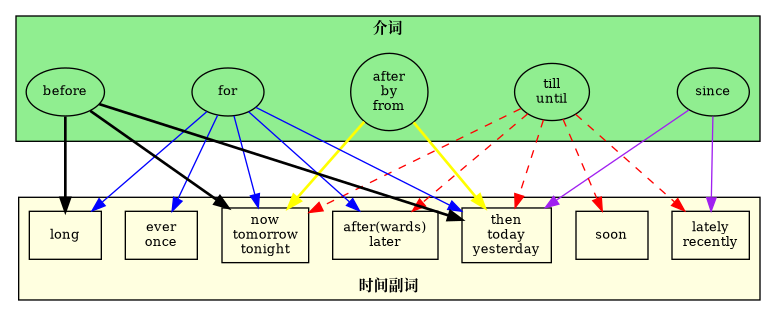
\includegraphics[width=\textwidth]{preptimeadverb.png}
  \caption{\label{fig:preptimeadv}最常用作介词补足语的时间副词}
\end{figure}


% #+BEGIN_SRC dot :file preptimeadverb.png :cmdline -Kdot -Tpng :exports results
%   digraph {
%     fontsize=11
%     fontname="serif bold"
%     rankdir="TB"
%     ranksep=0.8
%     node[shape=box fontsize=10]

%     subgraph  cluster_prep {
%       bgcolor="lightgreen"
%     rankdir="LR"
%       label=介词
%       node [shape=ellipse]
%       since
%       "B1_invis" [shape=none Xstyle=invis label="" fixedsize=true  width=0.4 height=.02]
%       till[label="till\nuntil"]
%       "B3_invis" [shape=none Xstyle=invis label="" fixedsize=true  width=0.4 height=.02]
%       afterl[label="after\nby\nfrom"]
%       "B2_invis" [shape=none Xstyle=invis label="" fixedsize=true  width=0.4 height=.02]
%       for
%       "B4_invis" [shape=none Xstyle=invis label="" fixedsize=true  width=0.4 height=.02]
%       before
%     }

%     subgraph cluster_adv {
%       bgcolor="lightyellow"
%     // rankdir="LR"
%     labelloc="b"
%       label=时间副词
%       lately[label="lately\nrecently"]
%       then[label="then\ntoday\nyesterday"]
%       now[label="now\ntomorrow\ntonight"]
%       afterr[label="after(wards)\nlater"]
%       soon
%       ever[label="ever\nonce"]
%       long
%     }


%     splines=false

%     since -> {lately, then}[color = "purple"]
%     till -> {lately,then,now,afterr,soon} [style=dashed color="red"]
%     afterl -> {then, now}[style=bold color="yellow"]
%     for -> {then, now, afterr, ever, long}[style=solid color="blue"]
%     before -> {then, now, long}[style=bold]
%   }
% #+END_SRC


\section{副词小品词up, down, back, away等}

down, in, up 等有时不是介词,而是副词。如以下句子中,左边介词(后接宾语),右
边为副词小品词(无宾语)。
\begin{taskitem}(2)
* I ran \unbf{down} the road.
* Please sit \unbf{down}.
* Something's climbing \unbf{up} my leg.
* She's not \unbf{up} yet.
* He's \unbf{in} his office.
* You can go \unbf{in}.
\end{taskitem}

这种短小的副词通常被叫作“副词小品词”,包括:about, above, across, ahead,
along, (a)round, aside, away, back, before, behind, below, by, down,
forward, home, in, near, off, on, out, over, past, through, under, up.

许多词既可用作副词小品词,也可用作介词,但也有例外: back, away (只能作副词小
品词); from, during (只能是介词).

副词小品词往往与动词连用,构成双词动词,有时会有全新意思(如break down, put
off, work out, give up),通常被叫做“\textbf{短语动词}”

副词小品词和形容词一样,往往用作be动词的补语。
\begin{itemize}
\item Why are all the lights \unbf{on}?
\item The match will be \unbf{over} by 4.30.
\item Hello! You're \unbf{back}!
\item I'm \unbf{off} – see you later!
\end{itemize}

\section{形容词和副词的比较级}

\subsection{可分等级的形容词和副词类型}

可分等级的形容词和副词可以有三种类型的比较,即:
\begin{description}
\item[向较高程度的比较] 通过屈折变化 -er 和 -est;迂回法 more和most的比较级、最高
  级表示(见\cref{tab:comparison})。

\item[相同程度的比较] 通过as/so \ldots{} as表示。
  \begin{itemize}
  \item Anna is \unbf{as tall as} Bill.
  \item Anna is not \unbf{as/so tall as} Bill.
  \end{itemize}

\item[向较低程度的比较] 通过little的比较级less 和最高级 least表示。
  \begin{itemize}
  \item This problem is \unbf{less difficult} than the previous one.

    这个问题比上题难度低。
  \item This is the \unbf{least difficult} problem of all.

    这是所有问题中最简单(不困难)的。
  \end{itemize}
\end{description}

\begin{table}[htbp!]
  \centering \small
  \begin{talltblr}[ caption = {形容词和副词的比较级},
    label = {tab:comparison},
    ]{
      width=\linewidth, colspec={llll},
      rowsep=2pt, colsep=4pt,
      row{1} = {font=\bfseries},
    }
    \toprule
    & 原级 & 比较级 & 最高级 \\\midrule
    \textbf{屈折变化形式} \\
    形容词 & high & higher & highest \\
    副词 & soon & sooner & soonest \\ \hline
    \textbf{迂回法形式} \\
    形容词 & complex & more complex & most complex \\
    副词 & comfortably & more comfortably & most comfortably \\
    \bottomrule
  \end{talltblr}%
\end{table}

\subsection{不规则的比较级、最高级形式}

不规则的比较级、最高级形式较少(见\cref{tab:composison})。

\begin{table}[htbp]
  \centering \small
  \begin{talltblr}[ caption = {不规则的比较级和最高级},
    label = {tab:composison},
    ]{
      width=\linewidth, colspec={lll},
      rowsep=2pt, colsep=4pt,
      row{1} = {c, font=\bfseries},
    }
    \toprule
    原形 & 比较级 & 最高级 \\  \midrule
    bad/sick/evil & worse & worst \\
    far(通用,进一步)& further & furthest  \\
    far (时空距离远) & farther & farthest \\
    good/well & better & best \\
    in & inner & innermost \\
    little & less & least \\
    many/much/a lot & more & most \\
    old & older/elder & oldest/eldest \\
    out & outer & outermost \\
    \bottomrule
  \end{talltblr}%
\end{table}

其中,farther/farthest 和 further /furthest 这两组词既是形容词又是副词。
farther/farthest主要只用来表达物理时空距离较远、最远。further /furthest则囊
括上述含义,并且还可以有“进一步,较多,最近” (more, additional, later) 的意思。
\begin{itemize}
\item I have to travel \unbf{further/farther} to work now.

  现在我得走更远的路去上班。

\item Let's consider this point \unbf{further}.

  让我们更深入地考虑这一点。

\item The school will be closed until \unbf{further} notice.

  学校将关闭,直至进一步的通知。
\end{itemize}

elder其实不是真正的比较级形式,因为在它后面不能跟 than,而要用规则屈折变
化older。elder只能指人,并多用在家庭成员出生顺序,如elder brother/sister表示
哥哥、姐姐。

\subsection{规则的比较级屈折变化}

\begin{itemize}
\item 以单个元音字母+单个辅音字母结尾的形容词,先双拼辅音字母,再加 -er和-est 。

  big \~{} bigger \~{} biggest \qquad sad \~{} sadder \~{} saddest

\item 以辅音字母 + y 结尾的形容词,先把 y 改为 i,再加 -er和-est。

  angry \~{} angrier \~{} angriest \qquad early \~{} earlier \~{} earliest

\item 词尾以哑音 -e 结尾,去掉 e,再加 -er和-est。

  pure \~{} purer \~{} purest \qquad brave \~{} braver \~{} bravest

  -ee结尾的去掉末尾的e,再加 -er和-est。

  free \~{} freer \~{} freest

\end{itemize}

\subsection{屈折法比较和迂回法比较之间的选择}
\begin{itemize}
\item 一般来讲,\textbf{单音节形容词通常用屈折变化}。

  例外是real, right, wrong 和介词 like只用迂回形式来构成比较级和最高级。

\item \textbf{大部分双音节形容词既可以用屈折变化,也可用迂回法。}

  对于以 -ing, -ed, -ful, -less等类复合词的双音节形容词来说,只能用迂回法。

\item \textbf{三个及以上音节的形容词,只能用迂回法。}

  带否定前缀 un- 的形容词两者都可用:
  \begin{itemize}
  \item unhappy \~{} unhappier / more unhappy \~{} unhappiest / most unhappy

  \item untidy \~{} untidier / more untidy \~{} untidiest/ most untidy
  \end{itemize}
\item \textbf{以 -ly 结尾的开放式副词可能因音节数量问题,不能用屈折变化,只能
    用迂回法。}
\end{itemize}

\subsection{比较级和最高级中the的用法}
\label{subsec:themost}

以下情况要加 the:
\begin{description}
\item[最高级作定语,修饰名词中心语,最高级前要加 the 或其他定
    指限定词。]
  \begin{itemize}
  \item Anna is \unbf{the/their youngest} child.

  \item Susan found \unbf{the most} blackberries.
  \item Della is \unbf{the/our most} efficient publisher.

    [efficient \doulos{/ɪˈfɪʃnt/} 效率高的;有功效的。]

  \item  John is \unbf{the shorter} of the twins.

    这个句子中虽然是比较级,可是 shorter在双胞胎之中充分指出说的是哪一位,所
    以仍然要有定冠词。
  \end{itemize}
\end{description}

以下情况不必加或不加 the:
\begin{description}
\item[than结构中的比较级] 一般不用加the。

\item[不与其他实体进行比较] 仅限于对某一实体的修饰,不特
  定,most不加the。\textbf{这里的most其实是限定词或增强语,而非迂回法比较级中
    修饰形容词、代表最高级的most副词。}
  \begin{itemize}
  \item \unbf{Most} books in my collection are science fiction.

  \item \unbf{Most} people can sing a little.

  \item Anna is \unbf{(the) youngest}.

  \item Mangoes are \unbf{(the) most} expensive in early summer.

  \end{itemize}

\item[重复和并列比较级] 表示程度逐渐增强,不加冠词。
  \begin{itemize}
  \item She is getting better and better.

  \item They are becoming more and more difficult.
  \end{itemize}
\end{description}

\item[形容词比较级或最高级作为副词]
  \begin{itemize}
  \item Speak \unbf{clearer}! [\unbf{more clearly}]
  \item This newsreader speaks \unbf{clearest} of all. [\unbf{most clearly}]
  \item It's \unbf{easier} said than done. [\unbf{more easily}]
  \item Ami ran \unbf{(the) slowest}.
  \item The car ran went (the) \unbf{slower and slower}.
  \end{itemize}

\item[已有冠词、所有格、人名或地理名称] 当名词短语中已有冠词、所有格代词、人
  名等中位限定词(中位限定词互斥,只可取其一,详见\cref{tab:determ},或地理名
  称在most前后时,已有足够限定功能,它\textbf{消除了限定词the的必要性}。
  \begin{itemize}
  \item She is \unbf{my best friend}.

  \item \unbf{Most of these people} can sing a little.

  \item I've read \unbf{most of Shakespeare}.

  \item The Romans conquered \unbf{most of England.} [conquered:
    \doulos{/rəʊˈmæn.tɪk/},征服]
  \end{itemize}
\end{description}


\subsection{比较级的前置修饰语}

形容词和副词的原级可为强化语(如 very, quite, so 等)所前置修饰。
\begin{itemize}
\item The job was \unbf{very easy}.
\end{itemize}

形容词和副词的比较级,不论是屈折变化形式,还是迂回形式,都可由增强
语(如 much, far 或 very much) 前置修饰:
\begin{itemize}
\item The job was \unbf{(very) much/far easier(more difficult)} than I thought.
\item She writes \unbf{(very) much/far better} than she used to.
\end{itemize}

下面是常常与比较级连用的其他强化语(和强化名词短语):
\begin{itemize}
\item somewhat/rather easier than \ldots{}
\item a lot/great/good/ easier than \ldots{}
\end{itemize}

\section{方法、状态的副词(Adverbs of Manner)}

\todo[inline]{副词分类这几节将来并入下一章状语。}

这一类的副词是修饰动词专用的,典型的拼法是形容词加上 \emph{-ly}字尾。既然它是修饰
动词的,那么原则上它的位置应该尽量和动词接近,通常是放在\textbf{动词后面}的位置。可
是,副词是修饰语,属于比较不重要的元素,\textbf{如果在句中有宾语、补语等主要元素存
  在时,方法、状态的副词就要向后挪,让宾语、补语等元素先出来。假如后移的结果
  造成副词与它所修饰的动词之间距离太远,那么也可以另辟蹊径,把方法、状态的副
  词调到动词前面的位置去,以维持修饰语必须和它所修饰的对象接近的原则。}以下分
别就五种基本句型举例说明。

\subsection{S+V}

\begin{itemize}
\item  \unct{The child}{S} \unct{giggled}{V} \unct{happily}{(adv.)} under the caress of its mother.

  小孩在母亲抚摸下笑得很开心。
\end{itemize}

介词短语 under the caress 在此先不讨论,留待后面章节来解说。本句中动
词giggled 之后已无主要元素存在,所以修饰动词的 happily可以直接放在动词后面。
当然,如果 happily 放在动词前面, 成为:
\begin{itemize}
\item  The child happily giggled \ldots.
\end{itemize}
仍然是正确的句子。在动词前面,也是紧邻动词的位置,所以符合修饰语要与修饰对象
接近的原则。但方法、状态的副词,除非有特殊原因,还是放在动词后面为佳,因为动
词是主要元素,先出来会比较清楚。

\subsection{S+V+C}

\begin{itemize}
\item \unct{He}{S} \unct{kept}{V} \unct{quiet}{C} \unct{resolutely}{(adv.)}.

  他坚定地保持沉默。
\end{itemize}
补语 quiet 是主要元素,要先出来,所以修饰动词的副词 resolutely就被挤到后面去
了。请注意,如果不这样处理,而把 resolutely放在前面,成为:

\begin{itemize}
\item He kept resolutely quiet.
\end{itemize}
这就会造成语意不清。因为副词也可以修饰形容词,读者会以为 resolutely是修
饰 quiet的修饰语,“坚定的沉默”。而同一句话有两种可能的解释,在修辞上就犯了
模棱两可(ambiguous)的毛病。这种错误在写作时要避免。有一种可以接受的位置是:
\begin{itemize}
\item  He resolutely kept quiet.
\end{itemize}
副词如果放在句尾,与动词之间会受到补语 quiet的阻隔,这时就可以把副词挪到动词
前面以维持它和动词的接近。而且resolutely 放在 kept的前面,并不会产生模棱两可
的毛病,所以是正确的位置。

\subsection{S+V+O}

\begin{itemize}
\item  \unct{He}{S} \unct{kissed}{V} \unct{the girl}{O} \unct{tenderly}{(adv.)}.

  他温柔地吻了那个女孩。
\end{itemize}
有宾语的句型,道理和有补语的句型一样,方法、状态的副词都会被挤到后面的位置。因而
tenderly 要放在 the girl 的后面。请注意下面的变化:
\begin{itemize}
\item  \unct{He}{S} \unct{passionately}{(adv.)} \unct{kissed}{V} \unct{the girl}{O} living next door.

  他热情地吻了那个住隔壁的女孩。
\end{itemize}
这个例子中,因为有一个简化的关系从句(以后会加以说明)living next door跟在
宾语后面,假如副词 passionately 再往后挪,不但与它所修饰的动词kissed 距离太远,
而且会有模棱两可的情形出现:
\begin{itemize}
\item  He kissed the girl living next door passionately.
\end{itemize}
这样处理的话,读者可能会认为 passionately 是修饰living,“热情地生活在隔壁”。
因为现在分词 living 原本是动词live,而且副词 passionately 又和 living比较接近。
这就必然会引起误解。如果把 passionately 放在宾语 the girl后面呢?
\begin{itemize}
\item  He kissed the girl passionately living next door.
\end{itemize}
还是不通!因为 passionately 紧临living,仍然会产生误解。这时,唯一的选择就是
把 passionately 放在动词kissed 的前面,才可以免除任何误解。

\subsection{S+V+O+O}

\begin{itemize}
\item  \unct{He}{S} \unct{showed}{V} \unct{us}{O} \unct{the document}{O} \unct{reluctantly}{(adv.)}.

  他很不情愿地把文件拿给我们看。
\end{itemize}

同样的,因为两个宾语都是主要元素,修饰语类的 reluctantly就被挤到后面去了。当
然,挪到动词前面也是一个办法,如:
\begin{itemize}
\item  \unct{I}{S} \unct{willingly}{(adv.)} \unct{offer}{V} \unct{you}{O} \unct{my help}{O}.

  我自愿对你提供帮助。
\end{itemize}
副词 willingly 放到句尾时会受到两个宾语 you 与 my help的阻隔,就有足够的理由
可以向前挪到动词 offer前面的位置,使它与动词没有距离。

\subsection{S+V+O+C}

\begin{itemize}
\item  \unct{They}{S} \unct{elected}{V} \unct{him}{O} \unct{chairman}{C} \unct{unanimously}{(adv.)}.

  他们全体一致推选他出任主席。
\end{itemize}
因为有宾语和补语这两个重要元素存在,副词 unanimously就要退让到后面。当然这会
使它和动词 elected之间产生距离,所以也有另外一个选择:
\begin{itemize}
\item  \unct{I}{S} \unct{happily}{(adv.)} \unct{pronounce}{V} \unct{you}{O} \unct{man and wife}{C}.

  我很高兴宣布你们结为夫妇。
\end{itemize}
这是牧师、神父证婚时必说的一句话。此言一出,男女双方的婚姻于焉生效。读者大概不曾听过把这句话的
happily 放在后面的吧?
\begin{itemize}
\item  I pronounce you man and wife happily.
\end{itemize}
这句话这样讲就感觉十分不对劲,原因何在?不是语法的问题。副词 happily被宾语与
补语挤到句尾去,这是语法正确的句型,可是修辞不佳。第
一,happily要和 pronounce相连,才足以表达那种欣喜的口吻。距离太远,语气就太冷
淡了。第二,全场宾客都在听的是man and wife这几个字,新郎新娘也在听这几个代表
终身大事底定的字眼,好进行拥吻。所以,man and wife 一定要放在句尾压轴的位置,
那么 happily 就只好往前挪了。

以上谈的是修饰动词专用的“方法、状态副词”,以及它在句中位置的变化原则。接下来看看其他种类的副词。

\section{强调语气的副词(Intensifiers)}

这一类副词有一个特色:它在使用上很有弹性,四种主要词类,包括名词、动词、形容
词与副词都可以用它来修饰。认识这一点,才算真正弄清楚形容词与副词间的分工。这
一类的副词又可以细分为以下三种:

\subsection{强调范围的副词(Focusing Adverbs)}

这一类的副词不多,典型的
像only、merely、also、especially、particularly、even等字就是这一类。它的功能
在于清楚界定出所谈事物的范围,好比照相机对焦(focusing)的动作一般。它的\textbf{位置
  要求很严格,有些要放在所修饰对象的前面,有些则要放在后面,但都不能和修饰的对
  象有任何距离。}因为它可以修饰任何词类,只要位置一变动,意思也就跟着发生变化。
以下举only 为例说明:
\begin{itemize}
\item I heard about the accident yesterday.

  我昨天听说了这件意外。
\item \unbf{Only I} heard about the accident yesterday. (No one else did.)

  只有我是昨天听说这件意外的。
\item \unbf{I only} heard about the accident yesterday. (I didn't it.)

  我昨天只是听说了这件意外。
\item I heard about \unbf{only the accident} yesterday. (I didn't hear anything
  else.)

  昨天全听人在讲这件意外。
\item I heard about the accident \unbf{only yesterday}. (I didn't hear about it
  earlier.)

  我直到昨天才听说这件意外。
\end{itemize}
这几个例子中,only 分别修饰代名词 I、动词 heard、名词 the accident与副
词 yesterday,可是都一样是当副词使用。

\subsection{加强语气的副词(Intensifiers)}

这是最典型的\textbf{Intensifiers}。它的位置通常要放在\textbf{修饰对象的前
  面}。例子:
\begin{itemize}
\item He is \unct{very much}{(adv.)} \unct{his father's son}{(n.)}.

  他和他爸一个调调
\item You're \unct{utterly}{(adv.)} \unct{insane}{(a.)}!

  你是完完全全疯了。
\item  I \unct{badly}{(adv.)} \unct{need}{(v.)} a drink.

  我亟需喝一杯。
\end{itemize}

\subsection{程度副词(Adverbs of Degree)}

这一类副词和加强语气的副词很像,但是程度副词是用来做“有几成”的表示,而非加
强语气。所以,如果把加强语气的副词去掉,只是语气变弱,意思不会变。但是如果拿
掉程度副词,意思则可能会发生改变,如:
\begin{itemize}
\item  The project is \unbf{almost} finished.

  计划已经差不多完成了。
\end{itemize}
这个句子中的 almost
就是程度副词,表示“八九成,还不到十足”的程度,并非加强语气。如果把它拿掉,就变成:
\begin{itemize}
\item  The project is finished.

  计划已经完成。
\end{itemize}
这个意思就和原文不同了。程度副词和另外两类的 Intensifiers一样,也是四大词类都可以修饰,
它的位置通常也是要放在修饰面。例如:
\begin{itemize}
\item You can buy \unct{practically}{(adv.)} \unct{anything}{(n.)} at a mall.

  在购物中心几乎什么都买得到。
\item I \unct{can}{(aux.)} \unct{hardly}{(adv.)} \unct{hear}{(v.)} you.

  我快听不到你在说什么了。
\item The promotion was \unct{moderately}{(adv.)}  \unct{successful}{(a.)}.

  促销活动还算成功。
\item I know your father \unct{rather}{(adv.)} \unct{well}{(adv.)}.

  我跟你父亲还算蛮熟的。
\end{itemize}

\section{修饰句子的副词(Sentence Modifiers)}

这又可以分成两类:\textbf{连接副词}和\textbf{分离副词}。这两类副词的位置,通常是放在句首,可是
也可以挪到主语、动词中间,甚至放到句尾位置。不论放在何种位置,都需要有\textbf{逗号}把
它和句子隔开来。这其中的原因我们分别来探讨一下。

\subsection{连接副词(Conjuncts)}

这一类的副词很像连接词(Conjunctions),有类似对等连接词 and 的(
如besides、furthermore),以及类似 but 的(如however、nevertheless)等等。它可
以连接两句话间的逻辑关系,可是缺乏连接词的语法功能,所以要用\textbf{标点}来帮忙。它的
变化很简单,请大家从例句中自行观察:

\begin{itemize}
\item Vivian Leigh is brilliant.

  费雯丽光芒四射。
\item C Gable, \unct{however}{(adv.)}, is lousy.

  克拉克·盖博却很糟。
\item \unct{Therefore}{(adv.)}, the film is less than perfect.

  影片因而并非十全十美。
\item  It is still a good movie; \unct{besides}{(adv.)}, good romances are rare these days.

  这部片子还是不错,况且近来好的文艺片不多了。
\end{itemize}

\subsection{分离副词(Disjuncts)}

把它归于修副词类是方便的分法。严格说起该是属于修饰另一句话的方法、状态副词。
请看例句:
\begin{itemize}
\item  \unct{Scientifically}{(adv.)}, the experiment was a success.

  从科学的角度来说,这个实验成功了。
\end{itemize}
固然 scientifically 可以说是修饰全句,可是深入一点来看,这个句子是下面这句的省略:
\begin{itemize}
\item  \unct{Scientifically}{(adv.)} speaking, the experiment was a success.
\end{itemize}
这个副词其实是修饰动词 speaking方法状态副词。更进一步把简化成下面的原貌:
\begin{itemize}
\item  If we are speaking \unct{Scientifically}{(adv.)}, the experiment was a success.
\end{itemize}
这个例子可以看出来,原来有两句话。第一句被简化成只剩一个方法、状态副
词scientifically,修饰“怎么说”,再附在第二句上。看到这个地步,就不难了解为
什么这个副词要有逗点隔开了——原来那是两个从句之间的逗号!分离副词也可以调到
中间的位置以及句尾可是仍然要有逗号隔开。请比较下面的例子:
\begin{itemize}
\item  You're not \unbf{answering} my questions \unbf{honestly}.

  你并没有老实回答我。
\item  \unbf{Honestly}, what are you going to do about it?

  老实说,你打算如何处置呢?
\end{itemize}
第一句的 honestly 是单纯的方法、状态副词,修饰动词 answer。第二句的honestly
则是分离副词,原本是 honestly speaking(老实说)。它是简化从句的残余,可以为
方便起见归于修饰全句的副词类。



\section{Test}

练习中有一些无关于观念、纯属辨字的问题,请仔细作答!

\paragraph{请选出最适当的答案填入空格内,以使句子完整。}

\begin{enumerate}
\item \ttu, he would leave his wife at home and go fishing himself.
  \begin{tasks}(2)
    \task More often than not
    \task Oftener than can't
    \task More often than doesn't
    \task Oftener than doesn't
  \end{tasks}

\item Separated for years, father and son found \ttu.
  \begin{tasks}(2)
    \task each other greatly changed
    \task one another greatly changed
    \task one another great changed
    \task one greatly changed another
  \end{tasks}

\item He speaks English \ttu as he does Chinese.
  \begin{tasks}(2)
    \task as fluently
    \task as fluent
    \task more fluently
    \task so fluent
  \end{tasks}

\item I don't like detective stories, but science fiction makes \ttu impression on me.
  \begin{tasks}(2)
    \task quite a different
    \task a quitely different
    \task a quite differently
    \task quitely a differently
  \end{tasks}

\item I am sorry. I \ttu forgot it.
  \begin{tasks}(2)
    \task clean
    \task cleanly
    \task cleanness
    \task cleanfully
  \end{tasks}

\item After walking so long a distance, I am \ttu tired.
  \begin{tasks}(2)
    \task dead
    \task deadly
    \task death
    \task died
  \end{tasks}

\item We are told to keep \ttu of the puddle of water.
  \begin{tasks}(2)
    \task clear
    \task clean
    \task clearly
    \task cleanly
  \end{tasks}

\item Dick went \ttu.
  \begin{tasks}(2)
    \task late yesterday there
    \task there late yesterday
    \task yesterday late there
    \task yesterday there late
  \end{tasks}

\item \ttu I like to be alone.
  \begin{tasks}(2)
    \task Some time
    \task Some times
    \task Sometime
    \task Sometimes
  \end{tasks}

\item \ttu spring, early one Saturday morning, I drove to Taiwan.
  \begin{tasks}(2)
    \task Latest
    \task Later
    \task Latter
    \task Last
  \end{tasks}

\item Both writing and rewriting \ttu are essential, if you want to make a hit.
  \begin{tasks}(2)
    \task careful
    \task carefulness
    \task carefully
    \task carelessly
  \end{tasks}

\item The computer plays an \ttu important role in modern life.
  \begin{tasks}(2)
    \task increasing
    \task increasely
    \task increased
    \task increasingly
  \end{tasks}

\item He exclaimed, "\ttu kind man before!"
  \begin{tasks}(2)
    \task Never I met with such
    \task I never meet with such
    \task Never I've met with a such
    \task Never have I met with such a
  \end{tasks}

\item "The workers in that factory are treated very badly." "Yes, they are \ttu than slaves."
  \begin{tasks}(2)
    \task the little better
    \task little better
    \task less better
    \task a small better
  \end{tasks}

\item "Is John very intelligent?" "Yes, \ttu than his brother,"
  \begin{tasks}(2)
    \task so much
    \task so more
    \task much so
    \task much more so
  \end{tasks}

\item The more we looked at the abstract painting, \ttu.
  \begin{tasks}(2)
    \task the more we liked it
    \task we liked it more
    \task better we liked it
    \task it looked better
  \end{tasks}

\item The girl was \ttu disappointed at how small the flower was.
  \begin{tasks}(2)
    \task noticeable
    \task noticed
    \task noticeably
    \task noticing
  \end{tasks}

\item With the computer down, we \ttu our work.
  \begin{tasks}(2)
    \task not longer would continue
    \task not longer could continue
    \task could continue no longer
    \task could no longer continue
  \end{tasks}

\item He threw the javelin \ttu than all the others.
  \begin{tasks}(2)
    \task farther
    \task as far
    \task further
    \task farthest
  \end{tasks}

\item The enemy is advancing. Stand \ttu.
  \begin{tasks}(2)
    \task firm
    \task firmly
    \task firmness
    \task to firm
  \end{tasks}

\end{enumerate}

\section{Answer}

\begin{enumerate}
\item (A) 动词部分有助动词 would,所以前面不能用助动词 doesn't(如 C 和 D)。又,more often than not 是一个常用短语,表示“经常”。
\item (A) 因是父子两人,故应用 each other。三人以上方能用 one another(如 B,C
  和 D)。答案 A 中,each other 是 found 的宾语,greatly changed 是宾语补语。
\item (A) 后面有比较级连接词 as,所以前面只能用 as(A 或 B)。空格位置应用副
  词 fluently 修饰动词 speaks,故选 A。D 的 so 一般用在否定句,例如 not so fluently 就可以配合后面的 as,作正确的答案。
\item (A) quite 是个强调语气的副词,可直接修饰名词短语 a different impression,故选 A。而 C 和 D 用了副词 differently,置于名词 impression 之前,词类错误。B 中的 quitely 错误,因为没有这种拼法。
\item (A) clean 作形容词是“干净的”,作副词时则是“完完全全”。在此用副词用法来修饰动词 forgot。
\item (A) dead tired 这个短语相当于“累得要死”,又 dead center 表示“正中红心”,在这两个短语中 dead 都当作强调语气的副词,不是形容词。
\item (A) keep clear of 意思是“避开,保持距离”,其中 clear 当 away 解释。

\item (B) 地方副词 there 在先,时间副词 yesterday 在后,这是一般的顺序。修饰 yesterday 的副词 late 置于它的前面。
\item (D) 这个位置要求频率副词(如 D,有时候)。A 的 some time 表示“一段时间”,
  是名词短语,如:I spent some time in the U.S.。B 的 some times 表示“某些时
  代”或是“若干次”。C 的 sometime 是个形容词,表示“从前的”,如 a
  sometime friend 是“从前的朋友”,当副词用时 sometime 表示“不特定的时间”,
  如 I’ll be back sometime。
\item (D) A 和 B 的最高级与比较级在上下文都没有呼应,C 的 latter 表示“后者”,上文应有“两者”时才能使用。
\item (C) 空格位置在 writing and rewriting 之后,应用副词类(C 或 D)修饰其中的动词部分。放在前面才能用形容词(如 careful writing and rewriting)。再看句意,应选肯定语气的 C。
\item (D) 这个位置是修饰形容词 important 的位置,应用副词(只有 D,而 B 是错误拼法)。
\item (D) 句尾的 before 暗示应用现在完成时最好(C 或 D),而 never 移至句首时应用倒装句,故选 D。
\item (B) little 是否定的语气,所以 they are little better than slaves 既表示“比奴隶好不了多少”,在此 little 作副词来修饰比较级的形容词 better。当然,只有形容词没有名词,就不应加冠词(如 A 和 D),而 C 的 less 本身是比较级,与 better 重复了。
\item (D) 回答是 He is much more intelligent than his brother. 其中用 much 来加强比较级 more intelligent。又,简答句中可以把重复的 He is intelligent 省略,只用 so 取代,即成 D。
\item (A) 这是双重比较结构(double comparison),以 the more…the more 之类的结构置于句首来取代连接词,表达“成正比”的关系,故选 A。
\item (C) 这个位置是副词位置,修饰 disappointed,只有 C 是副词。
\item (D) no longer 表示“不再”,作时间副词用,又有否定句功能,应与助动词 could 置于一起。

\item (A或C) 由下文 than 可看出是比较级, A 或 C 都可以,但在表示距离时更多
  用farther。另外further 可以额外表示“程度更深,
  更进一步”。

\item (A) stand firm 可作 you must stand firm 看待,这个 firm 是主语补语,应用形容词,修饰主语 you,意为“你们得保持坚定”,也就是“不要怕”。如果用副词 firmly,只能修饰动词 stand,意为“两条腿出点力气站稳”,与上文不大相配。
\end{enumerate}

\chapter{状语的语义和语法}

\section{状语按语义分类}

状语按语义可分为以下几类(也是状语的作用)
\begin{enumerate}
\item \textbf{空间}

  \begin{description}
  \item[位置] The dog was asleep \unbf{on the grass}.
  \item[方向] They walked \unbf{down the hill}.
  \item[目标] She hurried \unbf{to the station}.
  \item[来源] This book cannot be taken \unbf{from the library}.
  \item[距离] We mustn't go \unbf{very much further}.
  \end{description}
\item \textbf{时间}

  \begin{description}
  \item[固定时间位置] She was born \unbf{in 1980}.
  \item[前跨延续] I shall be in Chicago \unbf{until Thursday}.

    以“现在时间”为基点,向前跨越。
  \item[后跨延续] We have been at the airport \unbf{since yesterday}.

    以“现在时间”为基点,向前跨越。或者说从过去某时间点到现在。

  \item[时间频度] They \unbf{very seldom} went to see their parents.
  \item [一个时间和另一个时间的关系] She must \unbf{still} be in her office.
  \end{description}

\item \textbf{方式过程}

  \begin{description}
  \item[方式] The minister explained his policy \unbf{very clearly}.
  \item[手段] \unbf{By her insight}, she grasped the patient's real problem.
  \item[工具] I have difficulty eating \unbf{with chopsticks}.
  \item[施事] Penicillin was discovered \unbf{by Sir Alexander Fleming}.
  \end{description}

\item \textbf{方面}, 用状语增加具体真实价值。
  \begin{itemize}
  \item She helped him \unbf{with his research}.

    她帮助他做研究。
  \item He's busy writing.
  \end{itemize}
\item \textbf{原因}
  \begin{description}
  \item[原因] She died \unbf{of cancer}.
  \item[理由] He bought the book \unbf{through an interest in China}.
  \item[目的] He bought the book \unbf{to study English}.
  \item[结果] He always studies hard, \unbf{so he has good grades}.
  \item[条件] \unbf{If he always studies hard}, he will have good grades.
  \item[让步] \unbf{Even though he studied hard}, he didn't have good grades.
  \end{description}

\item \textbf{情态},可以使用状语来改变句子的真实性(如增强或减弱)。
  \begin{description}
  \item[强调] She \unbf{certainly} helped him with his research.

  \item[近似] They are \unbf{probably} going to the zoo.

  \item[限制] I shall be in Chicago \unbf{only} until Thursday.
  \end{description}

\item \textbf{程度},程度状语在改变句子的真实性上与情态状语类似,但是,程度状语添加了一
  个特殊的语义成分,可分等级性。
  \begin{description}
  \item[增强语义] He \unbf{badly} needed consolation.

    他急需安慰。badly在这里是非常,很,严重的意思。

  \item[减弱语义] She helped him \unbf{a little} with his research.
  \end{description}
\end{enumerate}

\section{可构成状语的词类}

状语成分可以由很多词类来实现:
\begin{description}
\item[封闭类副词为中心词的副词短语] \unbf{(Just) then}, the telephone rang.
\item[以开放类副词为中心词的副词短语] You should have opened it \unbf{(a bit more) carefully}.
\item[名词短语] They had traveled \unbf{a very long way}.
\item[介词短语] Tom hurried \unbf{across the field}.
\item[无动词从句] \unbf{When in doubt} the answer is ``no''. doubt, 疑问。
\item[非限定性从句] \unct{She}{S} \unct{realized}{V}, \unct{lying there}{A}, \unct{what she must do}{O}.
\item[限定性从句] We sent for you \unbf{because you were absent yesterday}.

  我们叫你来是因为你昨天缺席了。
\end{description}

\section{状语的位置}

与其他句子成分相比,状语成分可以比较自由地被置于句内各个不同的位置上(简单了
解即可):
\begin{description}
\item[I] \unbf{by then} the book should have been returned to the library.
\item[iM] The book \unbf{by then} should have been returned to the library.
\item[M] The book should \unbf{by then} have been returned to the library.
\item[mM] The book should have \unbf{by then} been returned to the library.
\item[eM] The book should have been \unbf{by then} returned to the library.
\item[iE] The book should have been returned \unbf{by then} to the library.
\item[E] The book should have been returned to the library \unbf{by then}.
\end{description}

如上文中的符号所示,状语可位于句中三个主要位置:句首位置I(NITIAL),句中位
置M(EDIAL),句末位置E(ND),但是,句中位置又分有三个变体(句中首位iM,句中中
位mM和句中末位eM)以及句末位置下分的句末首位(iE)。\textbf{句中位置就是紧接在功能词
  或系词后面的位置。}

若不存在功能词,那么M的位置就简单的处于S和V 之间;若S被省略,M的位置则位于V的
前面。

状语位置的选择由语义和语法因素来决定,但是同时也由信息处理的要求和末端
重 (end weight)原则来决定。如果没有特殊因素需要考虑,状语应被置于E(句末位
置),事实上,状语多数被置于这个位置。

\subsection{各类状语位置}

连接状语 Connecting adverbials 和评论状语 comment adverbials多表示本句与其他
句子的关系,或者评价本句,所以通常放在句首:
\begin{itemize}
\item \unbf{However}, not everybody agreed.

\item \unbf{Fortunately}, nobody was hurt.
\end{itemize}

Adverbials of indefinite frequency, certainty and completeness

不定频度状语(always, often等),确定性状语(probably, definitely等) 和完整性状
语 (completely, almost等) 通常放在句中。
\begin{itemize}
\item My boss \unbf{often} travels to America
\item I've \unbf{definitely} decided to change my job.
\item There is \unbf{clearly} something wrong.
\item The builder said he had \unbf{almost} finished, but it wasn't true.
\item \unbf{Sometimes} I'd like to live alone somewhere else alone.
\end{itemize}

焦点状语Focusing adverbials (also, just, even等)可以放在句中或其他位置,依具
体状语而定。
\begin{itemize}
\item He's \unbf{even} been to Antarctica.

\item We are \unbf{only} going for two days.


\item \unbf{Once} you could do a thing like that.

  只有你才会做出那样的事。
\end{itemize}

Adverbials of manner (how), place (where) and time (when) most often go in end position.

方式、地点和时间状语通常放在句中:
\begin{itemize}
\item She brushed her hair \unbf{slowly}.
\item The children are playing \unbf{upstairs}.
\item I phoned Alex \unbf{this morning}.
\end{itemize}

时间状语也可以放在句首。
\begin{itemize}
\item \unbf{Tomorrow} I've got a meeting in Cardiff.
\end{itemize}

强调状语Emphasizing adverbials (terribly, really等) 通常与其所强调的词放在一
起。
\begin{itemize}
\item I'm \unbf{terribly} sorry about last night.
\end{itemize}

程度状语 Degree adverbials (more, very much, most, a lot, so等) 据其功能位置可变

如有多条状语短句,通常按照方式、地点、时间的顺序排列。
\begin{itemize}
\item Put the butter \unbf{in the fridge} \unbf{at once}. (not … at once in the fridge.)
\item Let's go \unbf{to bed} \unbf{early}. (not … early to bed.)
\item I worked \unbf{hard} \unbf{yesterday}.
\item She sang beautifully \unbf{in the town} \unbf{hall last night}.
\end{itemize}

\subsection{分裂不定式}
\label{subsubsec:splitinf}

\begin{description}
\item[分裂不定式 (SPLIT INFINITE)] \index{概念!分裂不定式 split infinite} \textbf{句中末位状语}用在 to 和不定式的助动词之后,
  主要动词之前。
  \begin{itemize}
  \item He wasn't able to \unbf{even} move his fingers.
  \item She ought to \unbf{seriously} consider her position.
  \item She ought to have \unbf{seriously} considered her position.

    她应该认真考虑下自己的立场。

  \item Your task is to \unbf{really} understand your students' problems.
  \item I do TR\`Y to underST\'AND --- to TR\`ULY understand.

  \item No one invited me to \unbf{so much as} have a glass of water. [甚至]

    甚至没有人请我喝杯水。
  \end{itemize}
\end{description}

分裂不定式因文体在200多年里一直受到一些指责,但另一些专家认为这是可以接受的。

\chapter{语气}

语气(Moods)是利用动词变化来表达“真、假”口吻的方式。依各种不同程度的“真、假”口吻,可以细分为四种语气:
\begin{description}[style=standard, leftmargin=2em]
\item [叙述事实语气 (Indicative)] 表示所说的是真的。
\item [条件语气 (Conditional)] 表示真假还不能确定。
\item [虚拟语气 (Subjunctive)] 说反话,表示所说的与事实相反。或者表示现在时命
  令性语气,与间接祈式语气重合。
\item [祈使语气 (Imperative)] 表示希望能成真,但尚未实现。
\end{description}

四种不同的语气,看起来好像很复杂,不过各有各的重点,只要能掌握重点,便不难区
分,也不需死背。

\section{叙述事实语气}

一般的英语句子都是这种语气,读者从前在时态部分所学的现在式、未来式等等也叙述
事实语气,所以不必多作解释,其中只有未来式要说明一下。如:
\begin{itemize}
\item  I \unbf{will go} to the U.S. next year to study for an MBA degree.

  我明年要到美国去念企管硕士。
\end{itemize}
现在、过去的事情,是真是假已经可以确定,所以能用叙述事实语气。可是未来的事情
还没有发生,严格说起来还不能确定真假。这也就是为什么未来式动词中要加上助动
词will,因为\textbf{助动词都带有不确定的语气}。上例中如果说是事实语气,只能说
我确实有这个打算,计划到时候要去。至于明年会不会有变化,其实是无法预料的,这
和He went to the U.S. last year不同;过去的事情已经发生,可以肯定,所以能用叙
述事实的看下:
\begin{itemize}
\item  The weatherman says sunrise tomorrow \unbf{is} at 5:32.

  气象报告说明天日出是五点三十二分。
\end{itemize}
虽然是明天的日出,时间还没到,可是日出的时间可以用公式算出来。因为地球不会停
止转动,也不会忽快忽慢,所以“明天日出在以当作事实来必加上有不确定语气的will。
再看下一个例子:
\begin{itemize}
\item  The movie \unbf{starts} in 5 minutes.

  电影还有五分钟开演。
\end{itemize}
同样的,虽然还没开始演,可是时间表上排好了,“再过几分开演”就可以视为必用未
来式 will 来表示了。

未来式还有一个变化需要注意。请看下面的例子:
\begin{itemize}
\item  I\unbf{'ll be} ready when he \unbf{comes}.

  他来的时候我会有万全的准备。
\end{itemize}
\textbf{同时叙述到两件未来的事情,而两者之间有时间或条件的关联性时,往往其中一件(副
  词从句中的那件——何谓状语从句,将来会再作说明)要改成现在式。}这是因为两件
未来的事情都不确定,需要\textbf{先假定其中一件是事实,已经发生,在这个确定的基础上,才
  能推论另一件事。}上例中的 when he comes就是假定“他来”是确定的,用表示确定
语气的现在式 comes来叙述,然后才能那候我(I'll be ready)”一个例子的:
\begin{itemize}
\item  If you \unbf{are} late again, you\unbf{'ll be} fired.

  你再迟到就会被炒鱿鱼。
\end{itemize}
这是警告对方不得再迟到。下一次如果又迟到,这当然是未来的时间,\textbf{这件事是可以
  做成的,不应用假设语句。而应用叙述事实的语句,从而不适合用助动词},所以要改
成If you are late来表示。语法书中列出规则“表示时间或条件的状语从句要用现在式
代替未来式”,原因即在此。

\section{条件语气}

句子中一旦加上情态助动词(如:must、should、will/would、can/could、may/might
等),就产生了不确定的语气,称为条件语气。例如:
\begin{enumerate}
\item  You are right.

  你是对的。
\item  You may be right.

  你可能是对的。
\end{enumerate}
例 1 中是以现在式来叙述事实的语气。例 2 中因为加上了助动词may,就产生了不确定
性(“可能对”表示不一定对)。

情态助动词有以下两点需要注意:

\subsection{表达时间的功能不完整}

情态助动词中,must 和 should 这两个词在拼法上没有变化。至
于will/would、can/could、may/might这三对,虽然拼法有变化,可是并不表示时间,
而是语气的变化:每一对的后者比前者更不确定。例如:
\begin{enumerate}
\item The doctor thinks it \unbf{can be} AIDS.

  医生认为可能是艾滋病。
\item It \unbf{could be} anything---AIDS or a common cold.

  还看不出来是什么病——可能是艾滋病,也可能是感冒。
\end{enumerate}
例 1 中的 can be 是不确定语气,表示有这个可能,但还不一定。例 2 中的could be
并不表示过去式,两句话的时间一样,都是现在时间,差别在于 could表示更不确定的
语气。

\textbf{情态助动词,不论是 must 这一类,还是 can/could这一类,都无法明确表达
  过去式。}助动词后面要用不带to的不定式,同样缺乏时间变化,所以情态助动词要寻
找一种特别的方式来表达过去时间。

\subsection{用完成式表达对过去的猜测}

情态助动词用来猜测过去的事情时,因为缺乏表达过去时间的能力,所以要借助\textbf{完成式}
表达。例如:
\begin{enumerate}
\item  I \unbf{may rain} any minute now.

  随时可能会下雨。
\item  It \unbf{may have rained} a little last night.

  昨晚可能下过一点雨。
\end{enumerate}
例 1 是对现在、未来的猜测。如果要对过去(last night)做猜测,改成 might rain
并没有用,因为 might只表示更没把握的语气,并不是过去式。只有借助完成式 may
have rained(可能下过),才能表达对过去的猜测。

\section{虚拟语气}

虚拟语气有两种形式,传统上称为\textbf{现在时虚拟式}和\textbf{过去时虚拟式},
但是使用这些形式与其说和\textbf{时态}有关,不如说和\textbf{语气}有关。

\subsection{现在时虚拟语气}

现在时虚拟语气和祈使语气一样,用\textbf{动词原形}。因此,除 \textbf{Be} (虚拟
形式 be 和陈述形式 am, is 和 are 是有区别的)以外,\textbf{其他动词的虚拟语气
  形式只有在}\unbf{第三人称单数}\textbf{时才与陈述语气有区别}。

\begin{itemize}
\item I insist that we \unbf{reconsider} the Council's decisions. [陈述语气或虚
  拟语气,均可]
\item I insist that the Council \unbf{reconsider} its decisions. [第三人称单数未
  加 -s,使用动词原形,虚拟语气]
\item I insist that the Council's decision(s) \unbf{be} reconsidered. [动词原形
  be,虚拟语气]
\end{itemize}

\begin{description}
\item[命令性 (MANDATIVE)] 从句谓语使用\textbf{动词原形},用在that从句中。that从句由一
  个表示\textbf{要求、推荐、建议、决定、意图等}的先行词引导。这个词可以是动词、形容
  词或名词\footnote{命令性虚拟语气常用先行引导词:\\ 动词: decide, insist, move,
    order,
    prefer, request.\\ 形容词: advisable, desirable, fitting, imperative.\\
    名词: decision, decree, order, requirement, resolution.}:
  \begin{itemize}
  \item It's essential that this mission \unbf{not fail}. [\textbf{动词的否定形式
    不加助动词do,直接加入否定词not},虚拟语气]
  \item It's important that she \unbf{be} on time. [动词原形,未用 is,虚拟语气]
  \item (Even) if that \unbf{be} the official view, it can't be accepted.
  \end{itemize}

\item[套语式 (FORMULAIC)] 在传统和正式用法中使用的\textbf{固定短语},这些短语使用虚拟
  语气来表达\textbf{特定的愿望、祝福或要求}。虽然在现代口语中可能不常见,但它们在\textbf{特
    定的正式和仪式性场合}中仍然发挥着重要作用。简单举例,不需多了解:
  \begin{itemize}
  \item Long \unbf{live} the King. God \unbf{save} the Queen.
  \item \unbf{May} you succeed.
  \item Long \textbf{may} the sunshine.
  \item \unbf{Be that as it may}, we have nothing to lose.

    尽管如此,我们没有什么可输的了。
  \end{itemize}
\end{description}


\subsection{过去时间虚拟语气}

除了过去时间虚拟语气 \emph{if/as I/she/he/it were \ldots{} }之外,虚拟语气并不常见。

过去时间虚拟式简称为\textbf{WERE-虚拟语气} (WERE-SUBJUNCTIVE),使
用 were表示“\textbf{非事实}”的虚拟语气, 因此,\textbf{在过去时虚拟语气中只
  有第一人称和第三人称的单数形式才与陈述语气的形式不同},这是英语中真正虚拟语气动
词形式的唯一残余;且只能用在从句中:

\begin{itemize}
\item If I/he/she \unbf{were} leaving, you would have heard about it. [不用was,
  虚拟语气]

  如果他/她正要离开,你会听到这个消息。(非事实的虚拟假设,他/她没有离开。)

\item If I \unbf{were} you, I \unbf{wouldn't do} it.

  这句话选择用非事实的虚拟语气来说,是为了以缓和委婉的口吻劝对方不做事。当然,
  我不可能是你,所以不能用叙述事实的语气 I am you来表达。

  连带在主要从句中也用过去形态但不代表过去时间的 would来表示非事实,而成
  为 wouldn't do 的动词形态。

\item If I \unbf{were to take} the bribe, I \unbf{could never look at}
  other people in the eye again.

  我要是收下那笔贿款,就再也不能面对别人而问心无愧了。(我并没有收下)
\end{itemize}


\section{假设条件从句}

假设条件从句中的动词是时态后移的,\textbf{过去时形式用来指现在和将来时间,过去
  完成体形式用来指过去时间}(见\cref{tab:hypoverb})。当这些形式具有这
种\textbf{非事实的虚拟假设含义}时,我们把它们称为假设过去时 (HYPOTHETICAL
PAST) 和假设过去完成时 (HYPOTHETICAL PAST PERFECTIVE)。

\begin{table}[htbp]
  \centering
  \begin{talltblr}[ caption = {虚拟假设条件句中的动词时态},
    label = {tab:hypoverb},
    ]{
      width=0.9\linewidth, colspec={ccc},
      rowsep=2pt, colsep=4pt,
      row{1} = {font=\bfseries},
  }
  \toprule
  时间 & 条件从句 & 领句(主句) \\ \midrule
  现在和将来时间 & 过去时 & 过去时情态助动词\\
  过去时间 & 过去完成时 & 过去完成时情态助动词 \\
  \bottomrule
  \end{talltblr}%
\end{table}


\textbf{过去时间}的假设意义更加明确,相当于\textbf{对条件的隐含否定};而在
指\textbf{现在和将来时},假设意义可能仅仅表示\textbf{否定性的期待或假设,并不
  完全排除肯定的可能}。

假设条件语句与虚拟语气有\textbf{相似乃至重合}之处,对此也有很多争议。本笔记采
用夸克《朗文英语语法》将两者分隔开的做法,意图减少单一概念的分支数量,但夸克
说法确实\textbf{交错重合过多}!


\subsection{假设过去时}

假设过去时 (the HYPOTHETICAL PAST) 用于某些从句,尤其是 if条件从句中,表
示\textbf{和讲话人的信念或期待相反}的意思——现在或将来的某种状态、事件并没有出现。

\begin{itemize}
\item If she really \unbf{tried} / \unbf{were to try} harder next time, she \unbf{would pass} the examination.

  \textbf{指将来:but I expect she won't try harder.}

\item If an asteroid \unbf{should hit} the earth, man \unbf{could die} out.

  \textbf{指将来:如果小行星撞击地球,人类可能会灭绝。}

  \textbf{假设从句和领句均使用有过去形态、但不代表过去式的助动词来表示发生可能性很低,非事实。}

\item If I \unbf{should take} the money, \textbf{could} you \unbf{guarantee} secrecy?

  \textbf{指将来:万一我收下钱,你能保守秘密吗?(我不会收下钱。)}

\item If they \unbf{were} alive, they \unbf{would be} moving around.

  \textbf{指现在: but I assume they are not alive. 因第二人称与复数人称的过去时虚拟
    语气与陈述语气无法区分,这里既可当作虚拟语气,也可当作假设过去时。}

\item If she \textbf{were} trying harder, her parents \textbf{wouldn't be} so anxious.

  \textbf{指现在:but she don't try harder now.}

  \textbf{假设条件中如有动词的话,如想表达现在时间,似乎应使用动词的进行时态。}

\end{itemize}


\subsection{假设过去完成时}

领句中最常用的情态助动询是 would 。它用来表示假设的含义,不一定有任何其他情态
含义:
\begin{itemize}
\item If they \unbf{had invited} him to the conference, he \unbf{would have attended}.

  \textbf{指过去: but they didn't invite him.}
\end{itemize}

此外,还有以下例句指示过去:
\begin{itemize}
\item If I \unbf{had known} earlier, I \unbf{might have done} something.

\item I \unbf{might have married} her if she \unbf{would have agreed}.

  \textbf{情态助动词用于假设条件从句中时,和过去时及过去完成时结合在一起。}

\item If they \unbf{had asked} me, I \unbf{would have had to} speak.

  \textbf{have to 用来代替没有过去形式的 must.}

\item If I \unbf{had been} at home last night, I \unbf{should have heard} the noise.
\end{itemize}


\subsection{混合时间和真假的变化}

\textbf{假设复句的两个从句之间,时间可能不同,要分别判断}。例如:
\begin{itemize}
\item If I \unbf{had studied} harder \unbf{in school}, I \unbf{could qualify} for the job
  \unbf{now}.

  我在学校时要是好好念书,现在就可以符合这项工作的要求了。

  \textbf{假设从句是过去时间(在学校时)的假设,领句是现在时间(now)。}
\end{itemize}

\textbf{也可能混合假设与事实:假设从句为假设,用假设条件语法;领句为事实,用普通语法。}例
如

\begin{itemize}
\item I \unbf{could have contributed} to the fund drive then, only that \unbf{I
    didn't have} any money with me.

  我本来可以响应募款活动的,不过当时身上没带钱。
\end{itemize}

 以下例句前为事实,后为假设条件。
\begin{itemize}
\item It\unbf{'s} time we all \unbf{took} a rest.

\item I \unbf{wish} I \unbf{had} a memory like yours.

\item I \unbf{wish} this bus \unbf{went} to the university.

\item  If \unbf{only} I \unbf{had} more time!
\end{itemize}

\section{祈使语气}

祈使句又称为命令句。这种语气可视为是条件语气中,省略助动词来表示“希望能成真,
但尚未实现”。例如:Come in! 可以视为 You may come in! 的省略。

读者对祈使句都很熟悉,可是有一种间接要说明一下
\begin{itemize}
\item The court demands that the witness \unbf{leave} the courtroom.

  法官要求证人离开法庭。
\end{itemize}

如果法官直接对证人提出要求,他会说:
\begin{itemize}
\item  (You must) Leave the courtroom!

  离开法庭!
\end{itemize}
可是,若经由第三者转述这个祈使句,主语已经不是you,不能省略。但这仍然是祈使句
的语气,还不是事实,所以仍然省略掉must,用动词原形 leave 来表示祈使句语
气。\textbf{间接祈式语句其实与现在时命令性虚拟语气重合。}

再
如:
\begin{itemize}
\item There is a strong expectation among the public that someone \unbf{take}
  responsibility for the disaster.

  民众强烈期望有人为这件灾难负起责任。
\end{itemize}
这是一个期望,还不是事实(目前还没有人表示要负责),所以是祈使句的语气,要用动词原形
take 来表示。

一般语法书上是列出一些规则,如:
\begin{itemize}
\item  It is necessary that \ldots{} (有必要 \ldots{} \ldots)
\item  I insist that \ldots{} (我坚持 \ldots{} \ldots)
\end{itemize}

这些句型后面要用动词原形。一方面这些句型无法列得周全,另一方面也没有说明原因,
所以许多读者一直不能真正了解。其实在笔者的观察中,这就是一种祈使句,所以把它
称为“\textbf{间接祈使句}”,放在祈使语气中来介绍。

\section{结语}

语气的变化概如上述,如果读者从“用语气表示真假”为出发点,对四种不同的语气能
够有整体的了解,就不必死背很多规则。到目前为止,有关简单句的各项细节,包括复
杂的动词变化,已大致介绍完毕,只剩下介词。下一章我们要介绍的就是介词,把
简单句做一个收尾,之后就要进入复句结构了。

\section{Test}

\paragraph{请选出最适当的答案填入空格内,以使句子完整。}

\begin{enumerate}
\item The landlord demanded that he \ttu the rent by tomorrow.
  \begin{tasks}(2)
    \task pays
    \task pay
    \task paid
    \task has paid
  \end{tasks}

\item If you \ttu with her last night, there wouldn't be any misunderstanding between you now.
  \begin{tasks}(2)
    \task talked
    \task were talking
    \task could talk
    \task had talked
  \end{tasks}

\item \ttu to participate, I might have won First Place.
  \begin{tasks}(2)
    \task Had had the chance
    \task I had had the chance
    \task The chance had I had
    \task Had I had the chance
  \end{tasks}

\item That was a close call; you \ttu hit by the car.
  \begin{tasks}(2)
    \task could have been
    \task can have been
    \task could be
    \task can be
  \end{tasks}

\item If you had asked him, he \ttu the truth.
  \begin{tasks}(2)
    \task might tell
    \task would tell
    \task might have told
    \task had told
  \end{tasks}

\item They suggested that he \ttu it alone.
  \begin{tasks}(2)
    \task does
    \task do
    \task will do
    \task has done
  \end{tasks}

\item \ttu him, I would have spoken to him.
  \begin{tasks}(2)
    \task Had I known
    \task If I should have known
    \task If I know
    \task If I had been known
  \end{tasks}

\item I wish I \ttu there yesterday.
  \begin{tasks}(2)
    \task was
    \task were
    \task had been
    \task could be
  \end{tasks}

\item He would have made the speech, only that he \ttu a sore throat.
  \begin{tasks}(2)
    \task has
    \task had
    \task had had
    \task has had
  \end{tasks}

\item Even if he \ttu here, he couldn't have helped you.
  \begin{tasks}(2)
    \task has been
    \task had been
    \task was
    \task were
  \end{tasks}

\item \ttu you were coming, I would have got the contract prepared.
  \begin{tasks}(2)
    \task Had I known
    \task If I knew
    \task If I know
    \task Should I know
  \end{tasks}

\item If he should leave, everything would go to pieces. (Choose one sentence that has the same meaning as the above)
  \begin{tasks}
    \task He is going to leave, but there is nothing to worry about.
    \task Fortunately he's not leaving, for everything depends on him.
    \task Things will take a turn for the worse, and then he will leave.
    \task I hope he won't leave, but I'm afraid he has too much to do and can't stay.
  \end{tasks}

\item The boss demanded that all the letters \ttu without delay by seven tonight.
  \begin{tasks}(2)
    \task were typewritten
    \task be typewritten
    \task would be typewritten
    \task typewriting
  \end{tasks}

\item Choose the wrong sentence:
  \begin{tasks}
    \task They didn't stop to rest at each station because it would have slowed them down.
    \task It would have slowed them down to stop to rest at each station.
    \task Much as they would like to stop to rest at each station, they thought better of it.
    \task It was essential that they stopped to rest at each station, they thought better of it.
  \end{tasks}

\item If you don't finish this assignment on time, they \ttu you.
  \begin{tasks}(2)
    \task wouldn't have paid
    \task had not paid
    \task won't pay
    \task didn't pay
  \end{tasks}

\item I'll let you know the results when they \ttu.
  \begin{tasks}(2)
    \task come out
    \task will come out
    \task came out
    \task would have come out
  \end{tasks}

\item I'm not worried about security because I think he \ttu.
  \begin{tasks}(2)
    \task dares not tell
    \task dares not to tell
    \task doesn't dare tell
    \task doesn't dare to tell
  \end{tasks}

\item This door ought to \ttu a week ago.
  \begin{tasks}(2)
    \task have fixed
    \task be fixed
    \task get fixed
    \task have been fixed
  \end{tasks}

\item I am surprised that you \ttu so indiscreetly.
  \begin{tasks}(2)
    \task act
    \task should be acted
    \task should have acted
    \task could have been acted
  \end{tasks}

\item He said he \ttu disgrace.
  \begin{tasks}(2)
    \task would rather die than suffer
    \task chose death to
    \task would prefer death before
    \task would die rather than
  \end{tasks}

\end{enumerate}

\section{Answer}

\begin{enumerate}
\item (B) 这是间接祈使句,应用命令语气,即动词原形。
\item (D) 这是过去时间(last night)的非事实,为过去时间假设语句,应用假设条件过
  去完成时,故选 D。
\item (D) 从下文 might have won 可看出这也是过去时间假设条件,应用假设条件过去完
  成时:If I had had the chance to participate \ldots{} \textbf{省略掉连接词 If 时需
    倒装},故选 D。
\item (A) 从上句 was 得知是过去时间(a close call 意为千钧一发),后面的假设语
  句是过去时间,应用过去完成时情态助动词,故选 A。
\item (C) 从 had asked 可看出时间在过去,为过去时间假设语句,应用过去完成时情态
  助动词,故选 C。
\item (B) 从上下文可看出这是间接祈使句,应用动词原形,故选 B。
\item (A) 从 would have spoken 可看出是过去时间假设语句,故应用过去完成时,
  即 If I had known him,省略 If 后要倒装,即是 A。
\item (C) wish 表示这是非事实的愿望,要用假设语句或虚拟语气(两者相同)。时
  间 yesterday 是过去,应用假设过去完成时,故选 C。
\item (B) 从 would have made 来看是过去时间的假设语句(本来当时可以演说的)。然
  而\textbf{下文的 only that(不过)把语气反了过来,成为事实语气,所以要用简单过去
    式 B(he had a sore throat},他当时喉咙痛,这是事实,不用假设。过去时
  间就是过去式)。
\item (B) 从 even if 和 couldn't have helped 可看出这又是过去时间的假设语句,应
  用过去完成时,故选 B。
\item (A) 由下文 would have got 可看出是过去时间假设语句,故应用过去完成时 If I
  had known,再省去 If 用倒装句,即是 A。
\item (B) 原句意为“万一他要走了,一切都会完蛋。”因为主句从句都有过去时情态
  助动词,所以是假设语句,表示他要走的可能性很小,这和 B 的语气近似(还好他不
  走,因为全靠他了。)A 是“他会走,不过也不用怕。”C 是“事情会恶化,然后他
  才会一走了之。”D 是“我希望他不走,但恐怕他事情真的太多,不能留下来。”
\item (B) 由 demanded that 可看出这是间接祈使句语气,应用动词原形。
\item (D) A 中的 they didn't stop 是事实语气,it would have slowed them down(停
  的话会太慢)是假设语句。B 和 A 类似,只不过把停下改成不定式。C 的 much as
  they would like 表示 although they would like very much,而 they thought
  better of it 是“他们打消了那个念头”。D 的句型表示这是间接祈使句,可是动词
  却用 stopped,不是动词原形 stop,因而错误。
\item (C) 由上文 If you don't finish 可看出,\textbf{不是假设语句,而是普通条
    件语句,还有可能赶得完},用现在式来表示未来的可能情况,故下文要用未来式。
\item (A) 与上题相同,从 I'll let you know 可看出并非假设语句,所以要用现在式来
  表示未来可能的情况。
\item (D) dare 可作助动词,不过当助动词就不能加 \emph{-s},后面要接动词原形,例如 He
  dare not tell。这个词也可以作普通动词,不过当普通动词就不能直接加 not 作否
  定句,后面也不能再用动词原形,而应该如 He doesn't dare to tell。

\item (D) 时间 a week ago 是过去,而情态助动词 ought to 要表示相对的过去时间
  得用完成体来表示,故由 A 和 D 来选择。主词是 door,动词是 fix,应用被动态,
  故选 D。

\item (C) “你竟然做出如此草率的举动,真让我想不到。”这是说事情已经做了!同样的,
  助动词后面要加完成体来表示相对的过去时间,所以用 C(这句要用主动态)。
\item (A) rather than 就是一个比较级,than 是连接词,前后连接的部分要对称。如
  放在 would 之后,就会连接两个动词原形,故排除 D。答案 C 应为 would prefer
  death to (disgrace),答案 B 应为 would choose death over (disgrace),都是介
  词用错。

\end{enumerate}

\chapter{介词}

在英语语法中,介词可以说是最简单、也可以说是最难的东西。说它简单,是因为它
没有什么观念可言,不像时态、语气、句型等,要求系统性的理解,所以在介词的部
分,不会有“不懂”的问题。然而介词之难,也就难在它缺乏观念性,不能以一套观
念来涵盖所有介词的用法。英语中的介词虽然没有多少个,可是在短语中的用法却
变化多端。就算有多年英语写作经验的人,也可能用错。所以我们可以这样说:介词
的用法,比较接近单词、短语的问题,而不大属于语法的问题。

要想彻底了解介词的用法,最确实的方法是经由\textbf{泛读}来解决:培养阅读的习惯,快速、
大量、持续地阅读英语作品,例如把每个月的《TIME中文解读版》从头到尾看完。只要
看过各种介词的用法,阅读过无数的例子,假以时日,就会形成一些“感觉”。拿起
笔来写英语,自然可判断在哪个句子中该用哪个介词。其实不仅介词如此,单词与
语法句型的问题也都应该配合泛读来吸收大量的、反复的input,才能真正解决。


\section{介词短语}

所谓“介词短语”,就是由\textbf{介词加上一个名词短语所构成的意义单元},在句中
常被当做修饰语(形容词短语或副词用来修饰名词、动词与副词类。它的位置通常饰的
对象后面。例如:

\begin{itemize}
\item \unct{Cherries}{名词} are \unct{in season}{介词短语 } now.

  现在正是樱桃生产的季节。
\item Eggs \unct{are sold}{动词} \unct{by the dozen}{介词短语}.

  鸡蛋是论打出售的。
\item The box is \unct{full}{形容词} \unct{of chocolates}{介词短语}.

  盒子里装满了巧克力。
\item He'll return \unct{tomorrow}{副词} \unct{at the latest}{介词短语}.

  他最晚明天回来。
\end{itemize}

\section{介词补语}

\textbf{介词表达两个实体之间的关系,其中一个实体以介词补足语为代表。}

介词补足语通常都是名词性短语(含名词短语、代词、-ing从句、wh-名词性从句)。

介词短语本身也可以用作介词补足语,如:
\begin{itemize}
\item We didn't meet \unbf{until after the show}.

\item The weather has been fine \unbf{except in the north}.
\end{itemize}

\textbf{尽管that从句和不定式从句可以起名词作用,但是它们不能作介词补语。人称
  主格 I, you等也不能。}

\begin{itemize}
\item I was surprised $ \left\{
    \begin{aligned}
     &\text{\unbf{at} her angry response.}\\
     &\text{\unbf{at} hearing her objecti on.}\\
     &\text{\unbf{at} what she said.}\\
     &\text{to hear her objection.}\\
     &\text{that she responded so angrily. }
    \end{aligned}
  \right. $
\end{itemize}

\section{介词、连接词和动词}
\label{subsec:prepconn}

介词和连接词都具有关联或连接功能,试比较:
\begin{itemize}
\item The day \unbf{when} she arrived. [连接词]
\item The day \unbf{of} her arrival. [介词]
\end{itemize}

某些情况下,同一词项既可以作介词又可以作连接词,如\textbf{after, as, before, since, until}.
\begin{itemize}
\item the day$ \left\{
      \begin{aligned}
        &\text{\textbf{before} she arrived} [连接词]\\
        &\text{\textbf{before} her arrival} [介词]\\
      \end{aligned}
    \right. $
\end{itemize}

辨别这两个词类的一个标准是:介词引导的是\textbf{名词性或名词化补足语};而与之对应的连
接词(从属连词)引导的是一个\textbf{从句}。

\begin{table}[htbp]
  \centering
  \begin{talltblr}[ caption = {介词和连接词后面的结构},
    label = {tab:prepconn},
    ]{
      width=\linewidth, colspec={cccc},
      rowsep=2pt, colsep=4pt,
      row{1} = {c, font=\bfseries},
    }
    \toprule
    后接结构 & when连接词 & after连接词或介词 & by 介词 \\ \midrule
    限定从句 & when she spoke & after she spoke & \xout{by she spoke} \\
    非限定从句 & when speaking & after speaking & by speaking \\
    名词短语 & \xout{when her speech} & after her speech & by her speech \\
    \bottomrule
  \end{talltblr}%
\end{table}

有些分词( -ing 和 -ed)从句形式就可以有边缘介词 (marginal preposition)、非限
定动词形式的功能,又可以有连接词的功能,如 considering 和 given.

\begin{description}
\item[分词作介词] 接名词性(化)短语
  \begin{itemize}
  \item \unbf{Considering his age}, he has made excellent progress in his studies.

    [等同于 If one considers his age \ldots 或 In view of his age \ldots{}]

  \item \unbf{Given the present conditions}, I think she's done rather well.

    [等同于 If one takes into account \ldots{}。 take into account是习
    语 idiom:考虑到、顾及到]
  \end{itemize}

\item[分词作非限定性动词] 非限定性从句
  \begin{itemize}
  \item \unbf{Considering the conditions in the office}, she thought
  \end{itemize}

\item[分词作连接词]
  \begin{itemize}
  \item \unbf{Considering (that) he is rather young}, his parents have advised
    him not to apply.

  \item \unbf{Given (that) the weather is expected to be sunny tomorrow}, we should
    plan a picnic.
  \end{itemize}
\end{description}

其他可作连接词的现在分词形式还有seeing (that) 和 provided (that)等(连接词表
详见\cref{subsec:subcon})。


\section{介词后置}

\index{介词后置}
尽管介词一般在它本身补语的前面,但是,在一些情况下,介词必须后置:
\begin{itemize}
\item \textbf{介词动词}的\textbf{被动语态}结构,其中主语相当于主动语态里的介词
  补语:
  \begin{itemize}
  \item \unbf{The car} has been paid \unbf{for}.
  \end{itemize}

\item \textbf{介词补足语主位化}的不定式从句 或 -ing从句:
  \begin{itemize}
  \item \unbf{That man} is unpleasant to work \unbf{with}.

  \item \unbf{His advice} is not worth listening \unbf{to}.
  \end{itemize}

  因上,当疑问词或引导词是介词补足语时,介词往往出现在句尾,尤其是非正式用法
  中。
  \begin{itemize}
  \item \unbf{What} are you looking \unbf{for}?
  \item \unbf{Who} is she talking \unbf{about}?
  \item \unbf{About whom} is she talking? 太正式,日常不大用。
  \item \unbf{What} kind of films are you interested \unbf{in}?
  \item Tell me \unbf{what} you're worried \unbf{about}.
  \end{itemize}

  可是,当名词与疑问词连用一体时,介词不后置。
  \begin{itemize}
  \item \unbf{With} what money? (不能说 \sout{What money with.})
  \end{itemize}

\item 一些简单介词(如through)和多数的复杂介词(如because of, in addition
  to)不可以被后置。

\end{itemize}

\section{简单介词和复杂介词}

最普通的介词是一些单音节词项,如 at, for, in, on, to, with,\textbf{除非被后
  置},它们通常要\textbf{非重读且元音弱化}。

有一些多音节介词,它们中有的向来就是由单音节介词组成的复合词(例如: inside,
with in),有的源于分词(例如: during, concerning, granted),有的由其他语言引
入(例如: despite, except)。

介词数量的增加主要是由于介词与其他词组成了“\textbf{复合介词}”。复合介词主要
有两大类:
\begin{description}
\item[分词、形容词、副词、或连词 + 简单介词] 如:owing to, devoid of, away
  from, because of \ldots{}
\item[介词1 + 名词 + 介词2] 如:in charge of, by means of, at variance with,
  in addition to, as a result of \ldots{}
\end{description}


\section{按表示关系分类}

\subsection{表示空间关系的介词}

\begin{figure}[tp!]
  \centering
  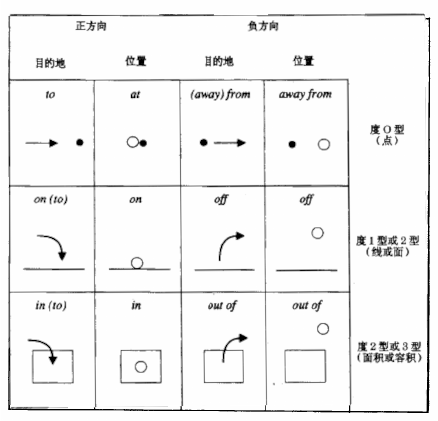
\includegraphics[width=0.8\textwidth]{prep1.png}
  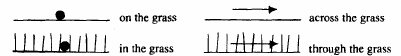
\includegraphics{prep2.png}
  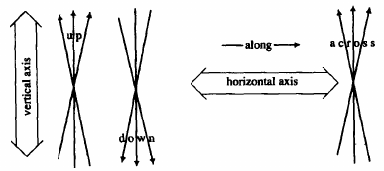
\includegraphics{prep3.png}
  \caption{\label{fig:preppic}表示空间关系的部分介词}
\end{figure}

\begin{description}
\item[over, under] 垂直关系,或者空间上接近。

\item[above, below] 仅表示“高于(低于)……水平上”

\item[among, between] among是在非分离的物体之中;between是在两独立物体之间:
  \begin{itemize}
  \item The house stands$ \left\{
      \begin{aligned}
        &\text{\emph{between} two farms.} \\
        &\text{\emph{among} farms.}
      \end{aligned}
    \right. $

  \item He likes getting \emph{among} people. [likes mixing with]
  \end{itemize}

\end{description}

其他略。

\subsection{表示时间的介词}

时间范围内一般只有两种度型,\textbf{时间点}和\textbf{时间段}。

\begin{description}
\item[时间位置 at, on, in, by]
  \begin{description}

  \item[at] 时间点和节假日
    \begin{itemize}
    \item at 6:30 pm, at the weekend, at noon, at Christmas

    \item 有些时间段被当作时间点来考虑,如:

      at night, at the/that time, at breakfast time
    \end{itemize}

  \item[on] 当作时间段看待的一天
    \begin{itemize}
    \item on Monday, on New Year's Day


    \item 时间有补足语时

      on the following day, on Monday morning, on Saturday afternoon, on the
      morning of 1 June

      但当补足语为early时,用in

      in the early morning, in the late afternoon
    \end{itemize}

  \item[in, during] 比一天更长或更短的时间段
    \begin{itemize}
    \item in the 18th century, in 1980, in August, in summer, in the evening

    \item during the 1990s, during Holy Week, during the night (during the = by)
    \end{itemize}
  \end{description}

\item[过去或将来时间段]
  \begin{description}
  \item[后置副词ago] 过去某一时间点之前的时间段

    \begin{itemize}
    \item We met \unbf{three months ago}.
    \end{itemize}

  \item[将来 in] 从现在起到未来之间的时间段
    \begin{itemize}
    \item We'll meet$ \left\{
        \begin{aligned}
          &\text{\emph{in three months' time}.} \\
          &\text{\emph{(in) three months from now}.} \\
        \end{aligned}
      \right. $
    \end{itemize}
  \end{description}

\item[持续时间段 for, during, over, (all) through, throughout]
  \begin{description}
  \item [for 持续整个时间段] for the summer

  \item[during 时间段中的某个时间段] during the (whole/stay) meeting

    如在during之后加whole/stay 修饰的话,则表示整个时间段。


  \item[over, through(out)] over通常和表示特殊日子的名词短语搭配,因
    此所指的时间一般比 through(out) 所指的更短。
    \begin{itemize}

    \item over the holiday/weekend/Sabbath, over holiday/night

    \item through(out) the summer
    \end{itemize}

  \end{description}
\item[before, after, since, till, until] 既是介词,有时连接词。

  作介词时,后面接:
  \begin{description}
  \item[时间名词短语] after next week
  \item[无主语 -ing 从句] since leaving school
  \item[从动词派生的或相当于从句的名词短语] till/until the fall of Rome,
    before the meeting
  \end{description}

\item[between \ldots{} and, by]
  \begin{description}
  \item[between \ldots{} and] 也表示时间段中的一个小时间段,还可以表示重复出
    现的相同事物之间的间隔。
    \begin{itemize}
    \item between 5 and 6 o'clock, between lunch and dinner

    \item  between meals/dances/acts/classes
    \end{itemize}

  \item[by] 事件结果出现的瞬间或时间终点。
    \begin{itemize}
    \item She should be back \unbf{by now}.

    \item \unbf{By the time} we'd walked five miles.
    \end{itemize}

  \end{description}
\item[不加时间介词的情况]
  \begin{description}
  \item[指示词last, next, this, that, some, every]
    \begin{itemize}
    \item last Thursday, next time, every month, this morning
    \end{itemize}

  \item[暗含 last, next, this指示意义的名词]
    \begin{itemize}
    \item today, yesterday, all (the) week
    \end{itemize}


  \item[时间介词可省略]
    \begin{itemize}
    \item (for) three months, (for) the whole time

    \item (on) the day before yesterday, (on) the next day
    \end{itemize}
  \end{description}
\end{description}


\subsection{表示原因和目的的介词}

\begin{description}
\item[原因、理由和动机 because of, on account of, for, out of]
  \begin{itemize}
  \item He lost his job \unbf{because of} his laziness.
  \item She was fined \unbf{for} dangerous driving .
  \item They died \unbf{from} exposure.
  \end{itemize}
\item[目的、目标和对象 for, to, at]
  \begin{description}

  \item[for]
    \begin{itemize}
    \item We had better set out \unbf{for} home.

    \item for money/love/shelter

    \item She made a beautiful \unbf{for her daughter}. [预计接收者]
    \end{itemize}

  \item[to] 实际接收者
    \begin{itemize}
    \item She gave a beautiful \unbf{to her daughter}.
    \end{itemize}

  \item[at] 暗示“希望达到某种目的”或有“敌意”
    \begin{itemize}
    \item kick/charge/bite/catch/shoot/chew at [目的不一定最终达成]
    \end{itemize}
  \end{description}
\end{description}

\subsection{表示由手段到刺激因素的介词}

介词还可以表示\textbf{手段}、\textbf{工具}用来回答 ``How?'' 问句,其中 by 可以表达使用的手
段, with 可以表达使用的工具,例如:
\begin{itemize}
\item I go to work \unbf{by} car.
\item The thief entered \unbf{by} the back door.
\item She won the match \unbf{with} her speed.
\item He managed to open the car \unbf{without} a key.
\end{itemize}

与手段和工具相反的是\textbf{施事者},施事者为\textbf{生物名词},可以引发某事。它可以用
介词 by 来表达。
\begin{itemize}
\item This picture was painted \unbf{by} Degas.

\item I was bitten \unbf{by} a neighbour's dog.
\end{itemize}

\subsection{表示材料、成分的介词 with, of, from}

\begin{description}
\item[with] 与“制作“动词 (verbs of ``making'') 连用,表示\textbf{其中一种成分};
  也可表示\textbf{遍布性}。
  \begin{itemize}
  \item This cake is made \unbf{with} lots of eggs.

  \end{itemize} paved \unbf{with} brick, filled \unbf{with} water, loaded \unbf{with} hay

\item[(out) of] 表示\textbf{整个东西的材料或成分};of还可以与表示“物质”的名
  词连用,作\textbf{后置修饰语和状语}:
  \begin{itemize}
  \item He made the frame \unbf{(out) of} wood. [Wood was the only material.]
  \item a bracelet \unbf{of} solid gold
  \item a heart \unbf{of} stone [比喻]
  \end{itemize}

\item[from] 表示\textbf{某物来源的一种物质}:
  \begin{itemize}
  \item Beer is made \unbf{from} hops.
  \end{itemize}
\end{description}

\subsection{基于某标准规格、方面或角色 for, at, as}

有些形容词隐含有比较等级:
\begin{description}
\item[for] 基于某\textbf{标准或规格}的形容:
  \begin{itemize}
  \item He's not bad \unbf{for} a youngster.

  \item The dog is long-legged \unbf{for} a chihuahua.
  \item It's a dreadfully expensive toy \unbf{for} what it is.
  \end{itemize}
\item[at] 基于\textbf{某方面}的形容:
  \begin{itemize}
  \item He's good/clever/brilliant/an expert \unbf{at} organizing things.
  \item He's bad/better/terrible/no good \unbf{at} games.
  \item She's getting on very well \unbf{at} her job.
  \end{itemize}

\item[as] 当as是“作为某个角色”的意思时,后面出现的短语表明了原因。
  \begin{itemize}
  \item \unbf{As} a doctor, I ought to help you.
  \end{itemize}
\end{description}



\subsection{from \ldots{} to / from \ldots{} through}

请看下例:
\begin{itemize}
\item The circus will be here four months, \unbf{from} May \unbf{to} September.

  马戏团要在这里表演四个月,从五月到九月。
\end{itemize}
由五月到九月,没有讲明日期,\textbf{可能是五月中到九月中},所以大概是四个月。但
是:
\begin{itemize}
\item The circus will be here five months, \unbf{from} May \unbf{through} September.

  马戏团要在这里表演五个月,从五月一直到九月。
\end{itemize}
through是“穿过”,所以用来表示起迄时间时,意思是“\textbf{头、尾皆包括在内}”,所
以是五月一日至九月卅日,包含整个的五月和九月,因而是五个月的时间。

\subsection{表示……的介词}

刺激和反应主要是用 at, with, about, in, of 和 to 来表达:
\begin{itemize}
\item I'm surprised \unbf{at/with} her attitude.

\item They were all angry \unbf{at/with} Tom for making such a stupid mistake.

\end{itemize}


其他略。

\section{介词副词}

有些介词还可以用作副词,常常像其省略了补足语的介词形式。

% Please add the following required packages to your document preamble:

% \usepackage{tabularray}
% \UseTblrLibrary{booktabs}
% \UseTblrLibrary{nameref}

\begin{table}[htbp!]
  \centering \small
  \begin{talltblr}[ caption = {可用作副词的介词},
    label = {tab:advprep},
    ]{
      width=\linewidth, colspec={lllll},
      rowsep=4pt, colsep=10pt,
    }
    \toprule
    aboard  & about   & above     & across    & after        \\
    ahead   & along   & alongside & around    & away         \\
    back    & before  & behind    & below     & beneath      \\
    besides & between & beyond    & by        & close        \\
    down    & east    & in(side)  & instead   & near         \\
    off     & on      & opposite  & out(side) & over(head)   \\
    past    & round   & since     & together  & through(out) \\
     up     & within  & without   & \SetCell[c=2]{l} under(neath)             \\
      \SetCell[c=3]{l} 复杂介词 in/on + 名词 \sout{+ 介词}        \\
    \bottomrule
  \end{talltblr}%
\end{table}

\begin{itemize}
\item A car drove$ \left\{
    \begin{aligned}
      &\text{past the door. [past 介词]} \\
      &\text{past}  [past 副词]
    \end{aligned}
  \right. $

\item Why didn't you come $ \left\{
    \begin{aligned}
	    &\text{before 7 o'clock? [before 介词]} \\
      &\text{before? [before 副词]}
    \end{aligned}
    \right. $

  \item Paul wants to go to the Zoo $ \left\{
      \begin{aligned}
        &\text{instead of staying home.} \\
        &\text{instead.}
      \end{aligned}
  \right. $
\end{itemize}


\section{Test}

\begin{enumerate}
\item For fear that we should run short of food \ttu the trip, we are carrying extra rations in the jeep.
  \begin{tasks}(2)
    \task at
    \task among
    \task in
    \task on
  \end{tasks}

\item \ttu imprecise calculations, the experiment was a failure.
  \begin{tasks}(2)
    \task Due
    \task Owing to
    \task Viewing
    \task According
  \end{tasks}

\item The children came rushing \ttu the sound of the circus parade.
  \begin{tasks}(2)
    \task on
    \task to
    \task at
    \task beyond
  \end{tasks}

\item Although too much leisure may lead people to a wasteful life, everyone has a right \ttu a minimum amount of leisure time.
  \begin{tasks}(2)
    \task with
    \task to
    \task on
    \task for
  \end{tasks}

\item In the sentence, "The size of the room is '12 × 14'," the sign "×" is to read "\ttu".
  \begin{tasks}(2)
    \task and
    \task with
    \task by
    \task cross
  \end{tasks}

\item The office is open Monday \ttu Saturday, and closed on Sundays.
  \begin{tasks}(2)
    \task since
    \task through
    \task also
    \task with
  \end{tasks}

\item John's parents died when he was only a child, and ever since he did not seem to have a home \ttu his own.
  \begin{tasks}(2)
    \task in
    \task of
    \task with
    \task at
  \end{tasks}

\item The dictionary is sold \ttu one hundred dollars a copy.
  \begin{tasks}(2)
    \task with
    \task by
    \task in
    \task at
  \end{tasks}

\item The workers are paid \ttu.
  \begin{tasks}(2)
    \task by the week
    \task with a week
    \task to a week
    \task since a week
  \end{tasks}

\item The experts know many things that won't work in curing AIDS, so they are that much closer to \ttu one that will.
  \begin{tasks}(2)
    \task find
    \task found
    \task finding
    \task have found
  \end{tasks}

\item \ttu prices so high, I'll have to do without a new suit.
  \begin{tasks}(2)
    \task With
    \task Because
    \task Because of
    \task As
  \end{tasks}

\item Mrs Johnson's old cat likes to sit \ttu the sun.
  \begin{tasks}(2)
    \task near
    \task in
    \task underneath
    \task below
  \end{tasks}

\item You can't do a hard day's work \ttu a cup of coffee and a slice of bread.
  \begin{tasks}(2)
    \task of
    \task on
    \task in
    \task at
  \end{tasks}

\item The necklace you are wearing is very becoming \ttu you.
  \begin{tasks}(2)
    \task at
    \task to
    \task for
    \task with
  \end{tasks}

\item In the photograph the man's face is \ttu focus and blurred.
  \begin{tasks}(2)
    \task out of
    \task with
    \task on
    \task to
  \end{tasks}

\item \ttu the seriousness of the occasion, the audience burst out laughing, at the extraordinary nature of the proposal.
  \begin{tasks}(2)
    \task Although
    \task Notwithstanding
    \task In respect of
    \task On behalf of
  \end{tasks}

\item \ttu being portable, a walk-man provides a high quality of sound.
  \begin{tasks}(2)
    \task Aside
    \task Far from
    \task Beside
    \task Besides
  \end{tasks}

\item George likes all vegetables \ttu for spinach.
  \begin{tasks}(2)
    \task except
    \task accept
    \task excuse
    \task expect
  \end{tasks}

\item \ttu the weather, forecast or anticipated, a true English gentleman always carries an umbrella, wherever he goes.
  \begin{tasks}(2)
    \task Regardless
    \task Regard
    \task Regard of
    \task Regardless of
  \end{tasks}

\item I welcome you most cordially, both personally and \ttu behalf of the faculty and the student body.
  \begin{tasks}(2)
    \task in
    \task at
    \task on
    \task to
  \end{tasks}
\end{enumerate}

\section{Answer}
\begin{enumerate}
\item (D) the trip 是一段时间,也是一条路程,可用 on 或 along。

\item (B) owing to 类似 because of,表示因果关系。A 和 D 都要加上 to 才能当短语用,C 的 viewing 不能当介词用,只有 considering 可以这样使用。

\item (C) 用 at the sound 表示“听到声音那一刻,马上就冲出来”。


\item  (B) a right to 表示“对于某事的权利”,是常用短语。

\item  (C) 表示长宽(面积)的“×”读为 by。

\item  (B) through 表示头尾包括在内,故一周中只有 Sunday 不开。

\item (B) 这是\textbf{双重所有格},以 a home of his own 的方式来同时表示 a
  home 和 his own home。

\item  (D) “以……之单价出售”,应用 at。

\item  (A) 每周计算应用 by the week。

\item (C) 空格前的 to 是 close to 的一部分,应当介词看待,因而要接动名词作宾语。

\item (A) with prices so high 是以介词短语方式来减化状语从句 because prices
  are so high。答案 C 的后面应改为 because of high prices 方可。答案 B 和 D
  都是从属连接词,可是这两词后面的从句缺了动词。

\item (B) 本句中 the sun 指阳光,是立体的范围,故用 in。
\item (B) on a cup of coffee…表示“只靠一杯咖啡……(来维持体力)”。
\item (B) becoming to one 表示“很适合某人(穿戴)”。

\item  (A) 因为下文说 blurred(模糊),故选 out of focus(没对好焦距)。
\item (B) 下文说观众哄堂大笑,前面则是“场合严肃”,故要表示“相反”的关系
  (A 或 B)。而 A 的 although 是从属连接词,不能连接名词短语 the
  seriousness,故用介词的 B。

\item (D) “除了”可手提,还可提供高品质音响。这个“除了”是“除了这还有那” 的
  意思,应用 besides。C 的 beside 是“在……旁边”,A 的 aside 是副
  词,B 的 far from 则是“决非……”。

\item (A) except for 表示“除了……以外”,表示“这个不算”。
\item (D) regardless of 是“不顾,不管”。
\item  (C) on behalf of 是“代表”。

\end{enumerate}

\chapter{主语--谓语一致}

\section{主谓一致和就近原则}

在英语中,最重要的一致关系类型是主语和谓语动词之间第三人称数的一致。单
数主语需要用单数动词,复数主语需要复数动词。

注意:在名词短语表示主语时,\textbf{由名词短语的中心词来决定名词短语的单复数}:
\begin{itemize}
\item \unbf{The change} in husbands' attitudes is most obvious in their families.
\item \unbf{The changes} in husbands' attitude are most obvious in their families.
\end{itemize}

从句、介词短语和副词作为主语一般算作单数:
\begin{itemize}
\item \unbf{Smoking cigarettes} \unbf{is} dangerous to your health .

\item \unbf{In the evenings} \unbf{is} best for me.
\end{itemize}

名字、标题、引文即使是复数名词短语,也算作单数。

\textbf{就近原则} (proximity) 是指\textbf{动词形式与紧靠在他前面的名词短语相
  一致}。如 either \ldots{} or \ldots{}, neither \ldots{} nor \ldots{}.
\begin{itemize}
\item Either your brakes \unbf{or your eyesight} \unbf{is} at fault.
\item Neither you, nor I, \unbf{nor anyone else} \unbf{knows} the answer.
\end{itemize}

在中国英语教学中,there be \ldots{} 也采用就近原则,但这其实是过时或者不准确
的,注意随机应变吧。
\begin{itemize}
\item There \unbf{is/are} an apple, two pears and some oranges on the table.
\end{itemize}

\section{主语是一个还是两个人(或物)?}

这部分主要讨论对等连接词 and 的判断。请比较:
\begin{mybox}
  \begin{itemize}
  \item   Ex. 1 Your brother John (have) come to see you.
  \item   Ex. 2 Your brother and John (have) come to see you.
  \end{itemize}
  句 1 中的 your brother 可以看出来就是John,是同一个人,所以是单数的主语,要用
  单数的动词。然而在句 2中一旦加上对等连接词,成为 your brother and John之后,
  就是两个人,是复数的主语,要用复数的动词。一般说来,对等连接词 and出现在主语
  中,往往表示主语有两个人(或物),所以应该是复数。
  \tcblower
  正确用法:Ex. 1 \textbf{has} \qquad\qquad Ex. 2 \textbf{have}
\end{mybox}

以上是大家都知道的判断原则。再下来就有了变化。请看:

\begin{mybox}

  \begin{itemize}
  \item   Ex. 3 The senator and delegate (want) to make an announcement.
  \item   Ex. 4 The senator and the delegate (want) to make an announcement.
  \end{itemize}
  senator 是参议员,delegate是代表。到底是一个人还是两个人要发表声明呢?本书前
  面曾讨论到名词短语,现在要用这个观念来帮忙了。

  名词短语有三个构成元素:限定词(包括冠词)、形容词与名词。其中任一元素都可省
  略。例如the rich 这个名词短语就只有限定词 the 和形容词rich,把名词(people)
  省略了。

  句 3 的主语 the senator and delegate 可视为一个名词短语。限定词只留一个the,
  名词部分则用 and 连接 senator 和delegate。这种情形应视为一个人,同时具有参议
  员和代表双重身分,所以是单数。

  \textbf{句 4 中的主语 the senator 和 the delegate各有限定词,需视为两个名词短语},因而
  是指两个人,动词也就该用复数。
  \tcblower
  正确用法:Ex. 3 \textbf{wants} \qquad\quad Ex. 4 \textbf{want}
\end{mybox}

因此限定词可以帮助判断名词短语的单复数。不过 every这个限定词又有不同的考量。
例如:
\begin{mybox}
  \begin{itemize}
  \item Ex. 5 Every man and every woman (have) to do something for the country.
  \end{itemize}
  句中主语 every man 和 every woman虽然各有限定词,是两个名词短语,似乎代表复数。
  不过再从意思上判断,man 和woman 是相对称的内容,指人的两种性别。重复 every是
  为了加强语气:不是指有两个人,而是表示不论男女,每一个“人”。亦即every man
  and every woman 的语气近似 man or woman,every“person”,所以应该选择单数的
  动词。
  \tcblower
  正确用法:Ex. 5 \textbf{has}
\end{mybox}

这个情况有点近似英语的一个成语:
\begin{mybox}
  \begin{itemize}
  \item   Ex. 6 All work and no play (make) Jack a dull boy.
  \end{itemize}
  主语 all work 和 no play 是两个名词短语(all 和 no都是限定词),似乎应为复数。
  不过从内容上来看,一天二十四小时都在工作(all work),就表示没有任何时间游戏
  (no play)。所以 all work and no play与其说是两件事,不如说是同一件事情的一
  体两面,重复是为了加强语气。因此动词应选单数。

  \tcblower
  正确用法:Ex. 6 \textbf{makes}
\end{mybox}

再看一个可以用限定词帮助判断的例子:
\begin{mybox}
  \begin{itemize}
  \item   Ex. 7 A cup and saucer (be) placed on the table.
  \item   Ex. 8 A cup and a dish (be) placed on the table.
  \end{itemize}
  句 7 中的 saucer 是放在咖啡杯下的小碟子,杯与碟可视为一组,所以主语中 a cup
  and saucer 只用了一个限定词a,当“一组咖啡杯”看待,是单一的名词短语,应作单
  数。

  句 8中的主语,一个是杯子,一个是菜盘子,这两件东西不能当一组看待,所以用 a
  cup and a dish 这两个名词短语来表示,因此动词要用复数。

  \tcblower
  正确用法:Ex. 7 \textbf{is} \qquad\quad Ex. 8 \textbf{are}
\end{mybox}

下面这个例子可釆同样原则,借助限定词来判断单复数,读者请自行练习一下:
\begin{mybox}
  \begin{itemize}
  \item   Ex. 9 A brown and white dog (be) at your doorsteps.
  \item   Ex. 10 A brown and a white dog (be) fighting over a bone.
  \end{itemize}
  \tcblower
  正确用法:Ex. 9 \textbf{is} \qquad\quad Ex. 10 \textbf{are}
\end{mybox}

以上所述大抵都可\textbf{借助限定词来观察一致性}。如果没有限定词呢?请看下例:
\begin{mybox}
  \begin{itemize}
  \item   Ex. 11 Bread and butter (be) not very tasty but very filling.
  \item   Ex. 12 Bread and butter (have) both risen in price.
  \end{itemize}

  bread 和 butter 都不可数,使用零冠词(zero article),因而看不到限定词。这时
  要从意思上判断单复数。句 11 说 bread and butter “不怎么好吃,但是吃得
  饱”。bread有人吃到饱,不过大概没有人只拿着 butter 吃到饱吧?所以这个句子中
  的 bread and butter应该是一种食品:吐司面包涂奶油。从意思上判断是单数,应用单
  数动词。

  句 12 中既然说 bread and butter “双双涨价”,自然是两种民生物资,应视为复
  数。

  \tcblower

  正确用法:Ex. 11 \textbf{is} \qquad\quad Ex. 12 \textbf{have}
\end{mybox}

下面这个例子也缺限定词,请读者练习:
\begin{mybox}
  \begin{itemize}
  \item   Ex. 13 Oil and water (do) not mix.
  \end{itemize}
  \tcblower
  正确用法:Ex. 13 \textbf{do}(油和水这“两种”物质无法混合。这是一句英语谚语。)
\end{mybox}

\section{主语是哪一个?}

这部分主要讨论主语中夹有对等连接词 or、but,以及比较级连接词 as、than时的判
断。
\begin{mybox}
  \begin{itemize}
  \item   Ex. 14 You want to borrow money? But I, as well as you, (be) broke.
  \end{itemize}
  一般语法书碰到这种状况又是列出规则叫人背,其实如果了解简化从句,根本不必背。
  这个句子可以还原为完整的句子:
  \begin{itemize}
  \item   I am broke as well as you are.
  \end{itemize}
  句中的第二个 as 就是比较级的连接词,前面的 I am broke 是主要从句,后面的you
  are 是从属从句。后者在比较级简化时可以把 be 动词省略,成为 as well as you,再
  把它向前移动,就变成句 14 的 I, as well as you了。由此可以看出,句 14 括弧中
  的动词属于主要从句,是 I 的动词,与 as well as you 无关。
  \tcblower
  正确用法:Ex. 14 \textbf{am}
\end{mybox}

下面这个例子也是同样的道理:
\begin{mybox}

  \begin{itemize}
  \item   Ex. 15 I, no less than you, (be) responsible.
  \end{itemize}
  这个句子可以还原为:
  \begin{itemize}
  \item   I am no less responsible than you are.
  \end{itemize}
  同样的,no less than yon are 这个比较级的句子可以简化,省略
  are,再往前移,所以句 15 的动词也应该依它的主语 I 而定。
  \tcblower
  正确用法:Ex. 15 \textbf{am}
\end{mybox}

以上是比较级连接词 than 和 as 的判断。接下来看对等连接词 but 的情形。\textbf{but这个
  连接词表达相反关系,连接的两部分通常是一个肯定,一个否定。在主语当中否定的部
  分等于被排除掉,动词要视肯定的部分而定},例如:
\begin{mybox}
  \begin{itemize}
  \item   Ex. 16 Everyone but a few complete idiots (be) able to see that.
  \end{itemize}

  主语当中用 but 来连接,等于排除掉后面 a few complete idiots
  的部分,因而动词要视 everyone 而定。
  \tcblower
  正确用法:Ex. 16 \textbf{was}
\end{mybox}

再看这个例子:
\begin{mybox}
  \begin{itemize}
  \item   Ex. 17 The eggs, not the hen, (be) stolen.
  \end{itemize}

  主语 the eggs, not the hen 里面虽然没有 but,可是意思、功能和 the eggs but
  not the hen 相同,后面的部分要排除(因为母鸡没被偷走,动词要跟 the
  eggs)。

  \tcblower

  正确用法:Ex. 17 \textbf{were}
\end{mybox}

下面这个例子比较复杂些:
\begin{mybox}

  \begin{itemize}
  \item   Ex. 18 Not only you but also I (be) at fault.
  \end{itemize}

  主语 not only you but also I 在意思上虽然是 you 和 I
  都算在内,不过语气偏重在 I 的部分。而且对等连接词前面的部分有
  not,表示形式上否定掉前面的 you,所以主语要跟后面的 I 走。

  \tcblower

  正确用法:Ex. 18 \textbf{was}
\end{mybox}

最后来看看对等连接词 or的判断。这个连接词表达的逻辑关系是“二选一”,不同
于 and表示“两边都算”以及 but表示“否定掉一个”。二选一该选哪一个做主语,完
全没有暗示,所以在用法上是\textbf{“选靠近动词的部分”做主语}。例如:

\begin{mybox}

  \begin{itemize}
  \item   Ex. 19 Either my father alone or both my parents (be) coming.
  \end{itemize}

  到底是父亲一个人来,还是父母亲一起来,完全没有暗示,只知道不会两者同时发生,
  要选一个。这时只能选靠近动词的both my parents 做主语。

  \tcblower

  正确用法:Ex. 19 \textbf{are}
\end{mybox}

下面这个句子差不多,请读者自行判断:
\begin{mybox}
  \begin{itemize}
  \item   Ex. 20 Neither he nor his friends (be) there at that time.
  \end{itemize}

  \tcblower

  正确用法:Ex. 20 \textbf{were}
\end{mybox}

最后这个句子要考虑一下:

\begin{mybox}
  \begin{itemize}
  \item   Ex. 21 (Do) he or his friends want to go?
  \end{itemize}

  这是疑问句,负责交代一致性的助动词靠近前面的 he,所以要选 he 做主语。

  \tcblower

  正确用法:Ex. 21 \textbf{Dose}
\end{mybox}

\section{主语中有 every、each、either、neither等表示“一”的字眼时}

只要有这些表示“\textbf{一}”的字眼在,后面有名词的话就得使用\textbf{单数名词},做主语时也就得用\textbf{单数动词}配合。这很容易了解,请读者自行练习:
\begin{mybox}

  \begin{itemize}
  \item   Ex. 22 Everybody (be) to report here tomorrow.
  \end{itemize}

  \tcblower

  正确用法:Ex. 22 \textbf{is}
\end{mybox}

\begin{mybox}
  \begin{itemize}
  \item   Ex. 23 Every student (have) several chapters to report on.
  \end{itemize}

  \tcblower

  正确用法:Ex. 23 \textbf{has}
\end{mybox}

\begin{mybox}

  \begin{itemize}
  \item   Ex. 24 Each (have) to make a five-minute speech.
  \end{itemize}

  \tcblower

  正确用法:Ex. 24 \textbf{has}
\end{mybox}

\begin{mybox}

  \begin{itemize}
  \item   Ex. 25 You (have) to make a five-minute speech each.
  \end{itemize}

  \tcblower

  正确用法:Ex. 25 \textbf{have}(each 在这里用作修饰语,主语是表示“你们”的yon,所以是
  复数)
\end{mybox}

\begin{mybox}

  \begin{itemize}
  \item   Ex. 26 Each of you (be) responsible for half of the job.
  \end{itemize}

  \tcblower

  正确用法:Ex. 26 \textbf{is}(这时主语是 each,原来的 you 变成介词 of的宾语,既
  然 each 当主语,就是单数)
\end{mybox}

\section{主语是关系代名词时}

\textbf{关系代名词代表其先行词。它本身没有单复数的变化,作主语时完全要看它代表的先行
  词是什么,借以判断一致性。}例如:

\begin{mybox}

  \begin{itemize}
  \item   Ex. 27 I don't trust people who (talk) too much.
  \end{itemize}

  关系从句 who (talk) too much 还原成单句就是 they (talk) too much,其中
  they 指的是前面的 people,所以动词等于是由 people 决定。

  \tcblower

  正确用法:Ex. 27 \textbf{talk}
\end{mybox}

下面这一组句子需要多考虑一下:
\begin{mybox}

  \begin{itemize}
  \item   Ex. 28 He has three options, which (look) equally attractive.
  \item   Ex. 29 He has three options, which (be) a good thing.
  \end{itemize}

  句 28 中的 which 应是代表先行词 three options(三项选择),这从关系从句的句
  意“看起来都一样吸引人”可以判断出来。因此它的动词应是复数。

  句 29 中的 which 则应解释为前面的整句话(he has three options),同样可以从句
  意看出来:他有三项选择可选,“这是一件好事”。

  which 既然代表一个句子,表示“那件事”,所以应该认定为单数。

  \tcblower

  正确用法:Ex. 28 \textbf{look} \qquad\quad Ex. 29 \textbf{is}
\end{mybox}

下面这个句子有两个地方需要分别判断:

\begin{mybox}

  \begin{itemize}
  \item   Ex. 30 It (be) the Johnson boys who (be) here last night.
  \end{itemize}

  主要从句的主语是个虚字 It。虽然补语是复数 the Johnson boys,可是动词得依主语
  而定,应用单数形式。后面的 who从句中主语代表的是先行词 the Johnson boys,所以
  动词要用复数。

  \tcblower

  正确用法:Ex. 30 \textbf{was}, \textbf{were}
\end{mybox}

\section{以单位做主语时}

\textbf{度量衡、时间、金钱等单位常以复数形态出现,做主语时却不一定要当复数看。}请看下例:
\begin{mybox}
\begin{itemize}
\item   Ex. 31 He makes eighty thousand dollars a year,which (be) a lot of
  money.
\end{itemize}

关系词 which 代表的是 eighty thousand dollars,看起来是复数。不过想一想,这并
不表示“八万个一块钱”的概念,而是有八万之多的“一笔钱”,所以要当单数看。

\tcblower

正确用法:Ex. 31 \textbf{is}
\end{mybox}

下面这个例子也差不多:
\begin{mybox}

\begin{itemize}
\item   Ex. 32 Ten seconds (be) quite a record for the 100--meter dash.
\end{itemize}

主语 Ten seconds只是量出一段时间,表示是百米短跑的一项优良纪录,并不是“十个
一秒钟”,所以要用单数动词。

\tcblower

正确用法:Ex. 32 \textbf{is}
\end{mybox}

\section{主语后面有介词短语时}

\textbf{一般说来,介词短语并不能影响主语是单数还是复数,所以在判断一致性时可以不
  去管它。不过有些情况还是需要留意。}

\subsection{一般情形}

\begin{mybox}
\begin{itemize}
\item  Ex. 33 Mrs. Lindsey, together with her sons, (be) on a European tour.
\end{itemize}

句中 her sons 是介词 with 的宾语,主语只有Mrs. Lindsey,所以虽然意思上是都
去了,不过这个句子主要在交代“这位太太”做了什么,要用单数。

\tcblower

正确用法:Ex. 33 \textbf{is}
\end{mybox}

下面这些例子也差不多,请读者自行判断:
\begin{mybox}
\begin{itemize}
\item   Ex. 34 The use of computers in business (be) now almost inevitable.
\end{itemize}

\tcblower

正确用法:Ex. 34 \textbf{is}(主语是 use)
\end{mybox}


\begin{mybox}
\begin{itemize}
\item   Ex. 35 There (be) a list of things to buy in the handbag.
\end{itemize}

\tcblower

正确用法:Ex. 35 \textbf{is}(主语是 list。手提包里只有单子,没有一堆东西。)
\end{mybox}

\section{主语为空的字眼时}

\textbf{如果主语是空的,只表达“全部/部分”的概念,看不出是什么东西,这时才要看后面的介词短语来判断单复数。}例如:
\begin{mybox}

\begin{itemize}
\item   Ex. 36 All of these (be) Lishan pears.
\item   Ex. 37 All of the money (have) been spent.
\end{itemize}

主语 all 是空的字眼,看不出是什么。如果后面是 of these(指梨山的梨子)就是复
数。如果接 of the money 就是单数。

\tcblower

正确用法:Ex. 36 \textbf{are} \qquad\quad Ex. 37 \textbf{has}
\end{mybox}

下面这句有点变化:
\begin{mybox}

\begin{itemize}
\item   Ex. 38 All but one of the pears (be) ripe.
\end{itemize}

主语中有对等连接词 but,它否定掉后面的 one,留下前面的 all 做主语。而all 的内
容由 of the pears 可看出是复数,所以要用复数动词。

\tcblower

正确用法:Ex. 38 are
\end{mybox}

下面这些例子判断的原则相同,读者可以试做看看。
\begin{mybox}

\begin{itemize}
\item   Ex. 39 A lot of the pears (be) damaged.
\end{itemize}

\tcblower

正确用法:Ex. 39 \textbf{are}
\end{mybox}

\begin{mybox}

\begin{itemize}
\item   Ex. 40 A lot of time (have) been wasted.
\end{itemize}

\tcblower

正确用法:Ex. 40 \textbf{has}
\end{mybox}

\begin{mybox}

\begin{itemize}
\item   Ex. 41 Half of the pears still (look) good.
\end{itemize}

\tcblower

正确用法:Ex. 41 \textbf{look}
\end{mybox}


\begin{mybox}

\begin{itemize}
\item   Ex. 42 Half of this pear (be) rotten.
\end{itemize}

\tcblower

正确用法:Ex. 42 \textbf{is}
\end{mybox}

\begin{mybox}
\begin{itemize}
\item   Ex. 43 Some of the cost (be) in transportation.
\end{itemize}

\tcblower

正确用法:Ex. 43 \textbf{is}

\end{mybox}


\begin{mybox}

\begin{itemize}
\item   Ex. 44 None of the pears (be) really good to eat.
\end{itemize}

\tcblower

正确用法:Ex. 44 \textbf{is} 或 \textbf{are}(none 是 not one,形状与意思都是单数,可采单
数动词。不过它也可算是空的字眼,由后面的复数of the pears决定它为复数,所以这
个字当主语时,单、复数动词都可以,也都有人用。)
\end{mybox}

\subsection{a number / the number 的判断}

\textbf{the number} 就是 that number,指的是一个数字,所以是\textbf{单数}。\textbf{a number},“某个数目
的\ldots\ldots{}”,则是指若干个可以数得出数目的东西,所以要用\textbf{复数}动词。例
如:
\begin{mybox}

\begin{itemize}
\item   Ex. 45 The number of people in the demonstration (be) five thousand.
\item   Ex. 46 A number of people (have) brought eggs to throw.
\end{itemize}

句 45 中 the number 是 five thousand的意思,为数目字,所以当主语时要用单数。
后者的 a number of people则相当于 some people,要用复数。

\tcblower

正确用法:Ex. 45 \textbf{is} \qquad\quad Ex. 46 \textbf{have}
\end{mybox}

\subsection{a pair of \ldots{} 的判断}

英语里有些东西习惯用 a pair of 来表示。如果主语是 a pair,就是 one
pair,那么应该是单数。例如:

\begin{mybox}

\begin{itemize}
\item   Ex. 47 A pair of pants (be) hanging on the wall.
\end{itemize}

\tcblower

正确用法:Ex. 47 \textbf{is}
\end{mybox}

不过英语里面要用 a pair 来表示的东西,像shoes、glasses、trousers、scissors 等
等,也可以直接说 these shoes\ldots{} 等,这时当然要用复数。

\begin{mybox}
\begin{itemize}
\item   Ex. 48 These pants (be) very fancy.
\end{itemize}

\tcblower

正确用法:Ex. 48 \textbf{are}(从这个句子中看不出 these pants是一条裤子还是几条裤子,
因为同样都要用复数形式。)
\end{mybox}

\section{集合名词}

结束了主语后面接介词的探讨,现在来讨论一下集合名词(Collective Nouns)。集
合名词在英语中不多,常见的只有\textbf{staff}(员工、幕僚)、\textbf{faculty}(教员)、以
及\textbf{family}、\textbf{police}、\textbf{committee}、\textbf{crew}(机员、船员)这几个字。这种词用
来表示“一个单位、集团”时要用单数动词,但是不加 \emph{-s} 而用来\textbf{表示单位内的“成
  员”时,要用复数动词}。例如:

\begin{mybox}
\begin{itemize}
\item   Ex. 49 The committee (be) studying the proposal.
\end{itemize}

这个句子中的 committee解释为委员会这个“会”也通(用单数动词),解释为会中
的“委员们”也通(用复数动词)。

\tcblower

正确用法:Ex. 49 \textbf{is} 或 \textbf{are}
\end{mybox}

不过有时候要从意思上作更精确的判断,例如:
\begin{mybox}

\begin{itemize}
\item   Ex. 50 The committee (be) five years old.
\end{itemize}

这时把 committee解释为委员们似乎不太通——太年轻了。应该是一个“单位”,有
五年历史了。

\tcblower

正确用法:Ex. 50 \textbf{is}
\end{mybox}


\begin{mybox}

\begin{itemize}
\item   Ex. 51 The committee (be) mostly Republican politicians.
\end{itemize}

从补语“大多为共和党政客”来看,主语 committee
应解释为“委员们”比较合理,所以要用复数。

\tcblower

正确用法:Ex. 51 \textbf{are}
\end{mybox}

\section{一些以 s 结尾的名词}

名词词尾的 \emph{s}不见得是复数,有些反而只能用单数形式,像有些代表学科、疾病的字眼
经常是如此。

例如:
\begin{mybox}

\begin{itemize}
\item   Ex. 52 Mathematics (be) my forte.

  数学我最拿手。
\end{itemize}

\tcblower

正确用法:Ex. 52 \textbf{is}
\end{mybox}


\begin{mybox}

\begin{itemize}
\item   Ex. 53 Mumps primarily (attack) children.

  腮腺炎好发于儿童。
\end{itemize}

\tcblower

正确用法:Ex. 53 \textbf{attacks}
\end{mybox}

还有一些要从意思来判断,例如:
\begin{mybox}
\begin{itemize}
\item   Ex. 54 Statistics (be) born in the gambling house.
\end{itemize}

主语 statistics 代表“统计学”,应用单数。

\tcblower

正确用法:Ex. 54 \textbf{was}
\end{mybox}


\begin{mybox}

\begin{itemize}
\item   Ex. 55 The statistics (be) not all accurate.
\end{itemize}

这时 statistics代表一批统计数字(才能说“并非全都正确”),所以要用复数。

\tcblower

正确用法:Ex. 55 \textbf{are}
\end{mybox}

以上所述,大致涵盖了处理一致性的所有重要原则。不过这方面的问题是知易行难。读者一定要多读多写,才能避免错误。

本章全用例题说明,因而不另附练习。


\chapter{替代形式和省略}

\section{替代形式}

\subsection{the same}

\begin{itemize}
\item A: Can I have \unbf{a cup of tea}, please?

  B: Give me \unbf{the same}, please.

\item Yesterday I felt \unbf{sad} and today I feel \unbf{the same}.

\item The Denison house is \unbf{small but very comfortable}, and ours is
  just \unbf{the same}.

\end{itemize}

\subsection{one, ones, some}

有两种替代形式的 one :一种复数形式是 some;另一种复数形式是ones。两种
都是\textbf{非重音}(因此与数字 one 区分),而且都替代\textbf{可数名词}。

some 也可以替代\textbf{不可数名词}。
\begin{itemize}
\item Have you any \unbf{knives}? I need a sharp \unbf{one}.
\item I like those \unbf{shoes}, but let's buy these \unbf{ones}.

\item Shall I pass \unbf{the butter}? Or have you got \unbf{some} already?
\end{itemize}


\subsection{so}

\begin{itemize}
\item You asked me to leave, and 'so I  \textbf{\textsc{d\`id}} .
\item You asked me to leave, and  I \textbf{\textsc{d\`id so}}.
\item A: It's starting to snow. B: 'So it \textbf{\textsc{\`is}} !
\end{itemize}

\section{省略}

\subsection{省略是省约的一种}

\textbf{省略} (ellipsis) 可以严格地被称为\textbf{语法省约} (grammatical omission),它有别于语
言中其他省约类型,譬如单词的\textbf{词首音节脱落} (apheresis) (cos = because , 'k
you = thank you,'d you = would you rather),\textbf{单词的截短法} (influenza = flu)
和\textbf{语义蕴含} (Frankly, \ldots{} )等。

省略与其他省约类型的区别主要在于,省略强调:
\begin{description}
\item[逐字还原 (VERBATIM RECOVERABILITY)] 能够精确恢复和重新某一段文字、发音
  和记录的内容。
\end{description}

但实际上,省略与其他省约方式仍有递差,其严格程度也有差别,并不存在完全分界线。

% Please add the following required packages to your document preamble:

% \usepackage{tabularray}
% \UseTblrLibrary{booktabs}
% \UseTblrLibrary{nameref}

\begin{table}[htbp!]
  \centering \small
  \begin{talltblr}[ caption = {省略标准的递差——从省略到其他省约},
    label = {tab:ellipsis},
    ]{
      width=\linewidth, colspec={cccccXl},
      rowsep=2pt, colsep=4pt,
      row{1} = {c, font=\bfseries},
    }
    \toprule a & b & c & d & e & 例句 & 省略类型\\ \midrule
    + & + & + & + & + & I'm happy if you are (happy). & 严格省略\\
    + & + & + & + & - & She sings better than I can (sing). & 标准省略\\
    + & ? & - & + & $\oplus$ & She works harder than him (*works). & 准省略\\
    + & + & + & - &  & (I am) Glad to see you. & 实境省略\\
    - & + & + & + & - & (Since he was / Being) Angry, he stalked out. & 弱省
    略\\
    + & ? & + & - &  & I believe (that) you are wrong. & 结构省略 \\
    - & + & + & - &  & The man (that/who/whom) I saw was half asleep. & 弱省
    略 \\
    - & ? & + & - &  & Houses (that/which are) owned by Mr Smith. & 弱省略 \\
    - & - & + & - &  & The door opened and (then/after that/\ldots{}) Mary
    entered. & 语义蕴含 \\ \bottomrule
    \SetCell[c=6]{l} \textbf{省略标准} \\
    \SetCell[c=6]{l} a: 省略词语可以准确还原。 \\
    \SetCell[c=6]{l} b: 省略的结构为语法“缺陷”。 \\
    \SetCell[c=6]{l} c: 还原词语后句子符合语法,且与原句意相同。 \\
    \SetCell[c=6]{l} d: 省略词语可根据篇章(而不是结构或实境)还原。 \\
    \SetCell[c=6]{l} e: 省略词语与先行词完全相同。\\ \bottomrule
    \SetCell[c=6]{l} \textbf{符号说明} \\
    \SetCell[c=5]{l} + \hspace{1em}符合标准 &&&&& $\oplus$ \hspace{1em} 适用
    标准须作语法变化 \hspace{2em} - \hspace{1em} 不符标准\\
    \SetCell[c=5]{l} ? \hspace{1em} 不确定  &&&&&  空白 \hspace{1em} 不涉及\\
    \bottomrule
  \end{talltblr}%
\end{table}

\subsection{省略的位置分类}

\begin{description}
\item[句首省略] (I) hope he's there.
\item[句中省略] Jill owns a Volvo and Fred (owns) a BMW.
\item[句尾省略] I know that we haven't studied hard yet, but we will (study hard).
\end{description}

\section{省略的还原类型}

\subsection{实境省略}

典型的实境省略是句首省略,尤其是采取\textbf{省略主语、功能词或两者都省略}这两个成
分的形式。

陈述句中的省略:
\begin{itemize}
\item (I) Told you so.
\item (I'm) Sorry I couldn't be there.
\item (It's) Good to see you.
\item (I'll) See you later.
\end{itemize}

疑问句中的省略:
\begin{itemize}
\item (Are you) In trouble?
\item (Is there) Anybody in?
\item (Do you) Want some?
\item (Have you) Got any money?
\item (Does) 'Anybody need a lift?
\item (Has) 'Jack done her homework?
\end{itemize}

\subsection{结构省略}

\begin{itemize}
\item I believe (that) you are mistaken.
\item We're staying there (for) another three weeks. [非正式]
\end{itemize}
\subsubsection{篇章省略}

\chapter{简单句}

\section{简单句和多重句}

\begin{description}
	\item[简单句 (SIMPLE)] 只有一个\textbf{独立从句}构成的句子。\index{概念!简单句 simple sentences}

\item[多重句 (MULTIPILE SENTENCES)] 有一个及以上从句作为句子的直接成分。还可以细分为:
  \index{概念!多重句 multiple sentences}
  \begin{description}
  \item[复合句 (COMPLEX)] \index{概念!复合句 complex} \textbf{从句}
    (SUBORDINATE CLASUSES) 作为一个(以上)句子成分,如直接宾语或状语;通常由
    一个从属连接词 (CONJUNCTION) 引导。

  \item[联合句 (COMPOUND)] 两个或两个以上\textbf{并列}从句 (COORDINATE
    clauses)。 \index{概念!联合句 compound}


    语法等级体系中相等地位的两个或两个以上的单位,可构成一个与之性质相同的单位。
    这种结构称为\textbf{并列关系} (COORDINATION), 而且像从属关系一样,由一个称
    为连词的连接词明确表示出来.这种连词叫\textbf{并列 (COORDINATING) 连词}。
  \end{description}
\end{description}


\improve[inline]{夸克的从句分类方法与其他一些语法书不同,比较复杂,暂且不论。}

关于从句结构和成分划分可以有一种以上的分析方法。因英语中遍布各处的递差造成较
多模糊性;通常这些模糊之处并不重要,只是需要建立自己较为自洽的分析方法。


例如:如对所有的介词短语来说,附加状语或补语的界限并不清楚。
\begin{itemize}
\item They were \unbf{out of breath}. \qquad  They were \unbf{breathless}.
\item She is/feels \unbf{in good health}. \qquad  She is/feels \unbf{healthy}.

\item She is \unbf{young} and \unbf{in good health}.
\end{itemize}

和本书不同,“简单句”这一术语在其他语法书中经常用来指一个不包含另一从句的独
立从句,而不管所包含的从句是不是句子的直接成分。有些语法书,把非限定结构(这
种结构含有一个非限定动词作为动词成分)看作是短语而不是从句。我们则把这种结构
看作是从句,因为可以把它分解为从句成分。非限定从句本身就是从属性质的,因此不
能成为典型的简单句形式


\section{否定}

\subsection{否定的三种类型}
\begin{description}
\item[从句否定 (CLAUSE NEGATION)] 从句法上将整个从句作为否定处理。

\item[局部否定 (LOCAL NEGATION)] 否定从句中某个成分。

\item[谓体否定 (PREDICATION NEGATION)] 一般指示用于某些助动词后面较次要的否
  定类型,否定主要动词及之后的部分(谓体)。
\end{description}

\subsection{从句否定}

\begin{description}
\item[动词否定] 最常见的形式。如无助动词,谓语部分加入假位 (dummy) 助动词be;
  在第一个助动词后加入否定词not。

\item[形式和意义上的否定] 使用no, not, never, none等否定一个从句成分,通过此
  方式来否定从句。

  正式文体中,否定整个从句的成分可以从它通常的位置移到句首。在这种情况下,主
  语和功能词常常需要倒装(见\cref{subsec:inversion})。


\item[意义否定但形式不否定的词] 如few, little, hardly, barely, scarely,
  rarely, seldom等词,也可实现从句否定:例如后面跟着非断定形式;或和肯定附加
  疑问句连用:
  \begin{itemize}
  \item I \unbf{seldom} get \unbf{any} sleep.

  \item \unbf{Hardly anyone} wants the job.

  \item They \unbf{scarcely} seem to care, \unbf{do they}?

  \item They \unbf{hardly} have any friends, \unbf{do they}?
  \end{itemize}

  当这些副词在文学和演说题材中作为状语或作为状语中的修饰语置于句首时,通常主
  语和功能词倒装:
  \begin{itemize}
  \item \unbf{Little did I} expect such kindness from so many.

  \item Rarely does crime pay so well as many people think.
  \end{itemize}
\end{description}

动词否定(左)和形式意义否定(右)的例句:
\begin{taskitem}(2)
  * That was \unbf{not} an accident.
  * That was \unbf{no} an accident.
  * He is \unbf{not} a friend of yours.
  * He is \unbf{no} friend of yours.
  * An honest man would \unbf{not} lie.
  * \unbf{No} honest man would lie.
  * She is\unbf{n't} a fool.
  * She is \unbf{no} a fool.
  * They are \unbf{not} staying with us \unbf{any} longer.
  * They are \unbf{no longer} staying with us.
  * I wo\unbf{n't} make that mistake ever again.
  * I will \unbf{never} make that mistake ever again.
\end{taskitem}

从句否定的一些特点:
\begin{description}
\item[否定从句后面附加补充从句]
  \begin{itemize}
  \item I haven't finished, \unbf{nor}/\unbf{and neither} have you. [附加否定
    从句]

    I've finished and \unbf{so} have you. [前后均肯定从句]

  \item I haven't finished, but Y\'OU H\`AVE. [附加肯定从句]

    I've finished, and \'YOU have T\`OO. [前后均肯定从句]
  \end{itemize}

\item[否定从句后跟赞同否定]
  \begin{itemize}
  \item ``He doesn't know Russian.'' ``N\`O, he D\`OESn't.''

    [比较: ``He knows Russian.'' ``Y\`ES, he D\`OES'']
  \end{itemize}

\item[either 和 too]
  \begin{itemize}
  \item She won't notice \unbf{any} change in you, \unbf{either}.

    [比较:She will notice \unbf{some} change in you, \unbf{too}.]
  \end{itemize}
\end{description}

\subsection{局部否定}

局部否定否定一个词或短语,而不否定从句。
\begin{itemize}
\item I visit them \unbf{not very often}.

\item \unbf{Not surprisingly}, they missed the train.

\item They live \unbf{not far} from us.

\item Our house has one wall with \unbf{no windows}.
\end{itemize}

\subsection{谓体否定}

情态助动词后停顿,强调not,用来否定谓体,而不是整个从句。

\begin{itemize}
\item They may / \unbf{'not go swimming}.

  [They are allowed not to go swimming.]

\item You can simply / \unbf{'not obey the order}.

\item She didn't / \unbf{'not like} them.
\end{itemize}

\subsection{否定的范围}

即使在从句否定中,否定成分以前的状语也通常不包括在否定范围之内。如:
\begin{itemize}
\item She definitely \unbf{didn't speak to him}.

  [她肯定没有跟他说话。]
\item She \unbf{didn't definitely speak to him}.

  [她不一定跟他说过话。]

\item I \unbf{wasn't L\v Istening} all the T\`IME.

  [我一直没有听。] 通过语调变化表明否定范围。

\item I \unbf{wasn't listening all the T\v IME}.

  [我不是一直在听。] 通过语调变化表明否定范围。

\item I \unbf{didn't listen} to \emph{some} of the speakers.

  我没有听一些人讲话,但听了另一些人讲话。
\item I \unbf{didn't listen to \emph{any} of the speakers}.

  我没有听任何人讲话。

\end{itemize}

\subsection{语音可表明否定的焦点}

英语语音中用于比较或突出重点信息的\textbf{重音焦点}可以表明否定和肯定的部分。
\begin{enumerate}
\item I \unbf{didn't take John to swim in the P\`OOL today}.

  [didn't do so]
\item I \unbf{didn't take J\v OHN} to swim in the pool today.

  [it maybe Mary]
\item I \unbf{didn't take John to SW\v IM} in the pool today.

  [just go to the pool, but they don't swim ]
\item I \unbf{didn't take John to swim in the P\v OOL} today.

  [may take John to the seaside]
\item I \unbf{didn't take John to swim in the pool toD\v AY}.

  [maybe yesterday]
\item \unbf{\v I didn't} take John to swim in the pool today.

  [someone else takes John to do so]
\end{enumerate}

还可以:
\begin{itemize}
\item I \unbf{didn't leave H\v OME} because I was afraid of my \unbf{F\`Ather}.
\item I \unbf{didn't leave home because I was afraid of my F\v Ather}.

  [I had left home, but it wasn't because of my father.]
\end{itemize}

\section{句子类型和话语功能}

简单句可以分为四种主要句法类型,并与话语功能息息相关。
\begin{description}
\item[陈述句] 句子有主语,并且主语位于动词前:
  \begin{itemize}
  \item \unbf{Richard} \unbf{gave} Tom a watch for his birthday.
  \end{itemize}

  另外,一些句子因情景中已暗含主语,省略了主语
  \begin{itemize}
  \item (I'm) Sorry I couldn't be there.

  \item (It's) Good to see you.
  \item (I'll) See you later.
  \end{itemize}

  另外 there/here be 陈述句中,主语在谓语 be 动词之后。这其实是存在句,
  见 \cref{subsec:behave}。

\item [疑问句] 一般分为如下两种:
  \begin{description}
  \item [一般 (yes-no) 疑问句] 如果没有助动词,则加一个假位助动词DO,如例句中
    的did;且将句子中的\textbf{第一助动词}前置于主语之前,:
    \begin{itemize}
    \item \unbf{Did} \unbf{Richard} \unbf{gave} Tom a watch for his birthday?

      疑问句通常在信息中心上用升调。上句可将升调放在watch或birthday,两者有着
      不一样的焦点。
    \end{itemize}

  \item [特殊 (Wh-) 疑问句] wh- 特殊疑问词位于句首,后接一般疑问句样式:
    \begin{itemize}
    \item \unbf{What} \unbf{did} \unbf{Richard} give Tom for his birthday?
    \end{itemize}
  \end{description}

\item[祈使句] 一般没有明显的主语,并且使用动词原形:
  \begin{itemize}
  \item \unbf{Give} Tom a watch for his birthday.

  \item \unbf{Let us all} \unbf{work} hard.

    宾格主语前加let,宾格后加动词原形。
  \end{itemize}


\item[感叹句] 句子由在名词短语中作\textbf{前位限定词的 what}, 或作\textbf{形
    容词、副词或从句强化语的 how} 及相关语句成分(如\textbf{宾语、补语、状语
    和主语})前置引导。

  wh- 成分可以是:
  \begin{description}

  \item[主语] \unbf{What a beautiful girl} came!
  \item[宾语] \unbf{What a fine watch} he received for his birthday!

  \item[补语] \unbf{How beautiful} she is!

  \item[状语] \unbf{How quickly} you eat!

    \unbf{What a long time} we've been waiting!

  \item[介词补足语] \unbf{What a mess} the room was in!
  \end{description}
\end{description}

\subsection{Wh- 疑问句}

Wh- 疑问句是由简单的疑问词协助构成的 (或 wh- 词),如: who/ whom/whose,
what, which, when, where, how, why。

\textbf{不同于 yes-no 疑问句的是,Wh-疑问句一般是降调。}

\textbf{带有 wh- 词的介词性补语}:
\begin{description}
\item[正式体]介词 + wh- 位于句首
  \begin{itemize}
  \item \unbf{To whom} should I write?
  \item \unbf{In which} city did you grow up?
  \item \unbf{At what} time does the train depart?
  \end{itemize}
\item[非正式体] wh- 位于句首
  \begin{itemize}
  \item \unbf{Whom} should I write \unbf{to}?
  \item \unbf{Which} city did you grow up \unbf{in}?
  \item \unbf{What} time does the train depart \unbf{(at)}?
  \end{itemize}

\item[工具、原因和目的] 就表示工具,原因,和目的的附加成分发问,wh- 位于句
  首
  \begin{itemize}
  \item \unbf{What} shall I mend it with?
  \item \unbf{What} are you fighting for?
  \end{itemize}
\end{description}

\subsection{其他疑问句}
\begin{description}
\item[否定的一般疑问句] 否定的疑问句,倾向于否定,但像一般疑问句一样回答。如:
  \begin{itemize}
  \item \unbf{Didn't} you believe me?

  \item \unbf{Aren't} you joining us this evening?

  \item \unbf{Haven't} he told you what to do?

  \item \unbf{Have} they \unbf{never} intited you home?
  \end{itemize}
\item[附加疑问句] 前半句为肯定或否定陈述句,后半句一般是相反的疑问。如:
  \begin{itemize}
  \item The boad \unbf{hasn't} left, \unbf{has} it?
  \item She \unbf{knows} you, \unbf{doesn't} she?
  \end{itemize}

  附加疑问句的核心语调落在助动词上,升调或降调表示不同倾向。夸克用 + 表示肯
  定,- 表示否定,如下:
  \begin{description}
  \item[+\`S -\'T] 附加疑问是升调,表倾向中性。如:
    \begin{itemize}
    \item He \unbf{likes} his J\`OB, \unbf{D\'OESn't} he?
    \end{itemize}
  \item[-\`S +\'T] 附加疑问是升调,表倾向中性。如:
    \begin{itemize}
    \item He \unbf{D\`OESn't} likes his J\`OB, \unbf{DOES} he?
    \end{itemize}
  \item[+\`S -\`T]
    \begin{itemize} 附加疑问是降调,倾向与陈述句一样。如:
    \item He \unbf{likes} his J\`OB, \unbf{D\'OESn`t} he? [肯定倾向]
    \end{itemize}

  \item[+\`S -\`T] 附加疑问是降调,倾向与陈述句一样。如:
    \begin{itemize}
    \item He \unbf{doesn't} like his J\`OB, \unbf{D\`OES} he? [否定倾向]
    \end{itemize}

  \item[+\`S + \'T] 比较少见的句式是陈述部分和附加疑问都是肯定,常有训斥或讽刺意味。如:
    \begin{itemize}
    \item Oh, you\unbf{'ve} had another \`ACcident, \unbf{H\'AVE} you?
    \item So that\unbf{'s} your G\`AME, \unbf{\'IS} it?
    \end{itemize}
  \end{description}


\item[回响疑问句] 重复部分或者是全部已讲过的话,以期得到确认。
\begin{itemize}
\item A: The Browns are emigrating. \qquad B: \unbf{\'Emigrating?}
\item A: He's a doctor. \qquad B: \unbf{Wh\'at} is he?
\item A: I'll pay for it. \qquad B: You'll \unbf{wh\'at}?
\item A: Have you ever been to BJ? \qquad B: Have I ever been \unbf{wh\'ere}?
\end{itemize}

\item[陈述疑问句] 随便文体,多用于口语;形式上和陈述句一致,句尾语调是疑问句
  的升调;希望得到听话人的认可。如:
  \begin{itemize}
  \item You've got a \unbf{D\'OCtor}?
  \item He didn't finish the \unbf{R\'ACE}?
  \end{itemize}
\end{description}
\part{中级句型——多重句}

\chapter{联合句或并列句}

\section{并列连词 and, or, but}

略。

\section{关联连词 both \ldots{} and, either \ldots{} or, neither \ldots{}
  nor}

if \ldots{} then, whether \ldots{} or 等\textbf{关联从属连词},暂且不表。

\begin{description}
\item[either \ldots{} or] 强调 or 的\textbf{排他} (EXCLUSIVE) 含义。
  \begin{itemize}
  \item \unbf{Either} the room is too small \unbf{or} the piano is too large.

  \item \unbf{Either} Sylvia \unbf{or} her sister will be staying with us.
  \end{itemize}

\item[both \ldots{} and] 强调 and 的补充 (ADDITIVE) 含义,前后并列同等。
  \begin{itemize}
  \item Mary \unbf{both} washed the dishes \unbf{and} dried them.

  \item \unbf{Both} Mary \unbf{and} Peter washed the dishes.
  \end{itemize}

\item[nor, neither] nor或 neither 可单独用作\textbf{否定补充副词},而不是作为一对关联
  连词。他们一般预先前文明示或暗示否定意义。
  \begin{itemize}
  \item She doesn't like them and \unbf{nor} does her brother.

  \item ``I'm not going.'' ``\unbf{Nor} am I.''
  \item They never forgave him for the insult, and/but \unbf{neither/nor} could he rid
    himself of the feelings of guilt for having spoken in that way.
  \end{itemize}


\item[关联连词 neither \ldots{} nor]
  \begin{itemize}
  \item David \unbf{neither} loves Joan, \unbf{nor} wants to marry her.

  \item \unbf{Neither} peter \unbf{nor} his wife wanted the responsibility.
  \end{itemize}


\item[not (only) \ldots{} but] 不但 \ldots{} 而且
  \begin{itemize}
  \item Columbus \unbf{not only} plays hard \unbf{but also} works hard.

  \item Not only did they break in to Mr. Zhang's office, but they also stole his books.

    为加强语气,可将Not only倒装于句首,后接表强调的助动词DO + 主谓从句。

    因为传统语法认为\textbf{并列从句彼此要功能和地位相等},所以Not only倒装时,
    前后都是完整句子 they \ldots{}
  \end{itemize}
\end{description}

\section{准并列连词}
\label{subsec:quasicoor}

\begin{description}
\item[准并列连词 (QUASI-COORDINATORS)] \index{概念!准并列连
    词quasi-coordinators} 有时候像\textbf{并列连词},有时候又像\textbf{从属连词}或\textbf{介词}。他们有:
  \begin{description}
  \item[比较形式] as well as, as much as, rather than, more than

  \item[关联连词] not so much \ldots{} as
  \item[其他] if not, not to say
  \end{description}
\end{description}

少见,略。


\chapter{复合句}

\section{从句和领句}

一方面,\textbf{复合句}像简单句,因为它\textbf{只包含一个主要从句};但另一方
面,它\textbf{有一个或一个以上的从句作为它的句子成分。}

\textbf{从属和并列}相互结合可使句子更加复杂,结构更加多变。复合句的每一个主要
从句可能包含一个或多个从句,而每个从句有可能包含自己的从句。

\begin{itemize}
\item Although I admire her reasoning, \unbf{I reject her conclusion}.
\end{itemize}

夸克使用\textbf{领句} (MATRIX clause)来称呼去除了从句的领句。

从句的三种主要类型见 \cref{subsec:iffinite}。

\section{限定性、非限定性动词和从句}
\label{subsec:iffinite}

\subsection{限定性和非限定性动词}

在英语语法中,动词可以分为限定性动词(finite verbs)和非限定性动词
(non-finite verbs)。\index{概念!限定性动词@限定性动词,finite
  verbs}\index{概念!非限定性动词@非限定性动词,non-finite verbs}
\begin{description}
\item[限定性动词] 受\textbf{主语、时态和语气}等因素影响的动词。这类动词
  \textbf{可以独立构成谓语},可以明确表明时态、人称和数的不同。具体特点是:
  \begin{description}
  \item[时态明确] 表示动作发生的时间(如过去、现在、将来)。
  \item[与主语一致] 动词形式会随着主语的人称和数的不同而变化。
  \item[可单独作为谓语] 在句子中,限定性动词通常是谓语动词。且\textbf{只有谓语动
      词中的第一个动词是限定性的}。
  \end{description}


\item[非限定性动词] \textbf{不受时态、人称和数等因素影响的动词形式。它们不能
    单独作为句子的谓语},通常需要与其他动词搭配使用。有以下三种形式:
  \begin{description}
  \item[不定式 (INFINITIVE)] 通常以 to 开头,如 to eat、to run。不带 to 的不
    定式谓语较少见,但也有:
    \begin{itemize}
    \item \unbf{Rather than you do the job}, I'd prefer to finish it myself.
    \end{itemize}
  \item[分词 (PARTICIPLES)] 包括现在分词 (eating) 和过去分词 (eaten)。
  \item[动名词 (GERUND)] 动词加 -ing 构成,具有名词的功能,如 running。
  \end{description}
\end{description}

\subsection{从句的结构分类}

夸克认为\textbf{从句}有三种主要的结构类型:
\begin{description}
\item[限定性从句 (FINITE CLAUSE)] \index{概念!限定性从句 finite clause} 谓语
  带有一个限定性动词短语的从句。
\item[非限定性从句 (NONFINITE CLAUSE)] \index{概念!非限定性从句 non-finite
    clause} 谓语带有一个非限定性动词的从句。
\item[无动词从句 (VERBLESS CLAUSE)] \index{概念!无动词从句 verb-less clause}不含动词成分,但仍然可分析为从句成分的分
  句。如:
  \begin{itemize}
  \item \unct{Although}{连词} \unct{always}{A} \unct{helpful}{V}, he was not much liked.
  \end{itemize}
\end{description}

\section{形容词性关系从句}

一般我们说关系从句时,就是指形容词性关系从句。可根据关系从句与其先行词的关系,
将之分为限制性和非限制性两种。

\textbf{关系代词引导形容词性关系从句,总是放在关系从句开头。有which, who,
  whom, whose, that 或零关系代词,他们都可以作限制性关系代词,但that或零不能
  做非限制性关系代词。}

\textbf{1. 限制性关系从句与它们的先行词或中心词在读音上是一气呵成的,以示对先行词所指
  对象的限制。}
\begin{itemize}
\item This is not \unbf{something} \unbf{that/which} would disturb me \`{A}NYway.

  无论如何,这都不会打扰我。(something that \ldots{} me连读)
\item I'd like to see \unbf{the car} \unbf{that/which/( )} you bought last week. (zero由( )表
  示)

  我想看看你上周买的那辆车。(the car that/which \ldots{} last week连读)
% \item The lady \unbf{whose} daughter you met is Mrs. Brown.

%   你见过她女儿的那位女士是布朗夫人。
\end{itemize}

\textbf{2. 非限制性关系从句是一种插入性说明,它通常是对先行词加以描述而不是对先行词作进一
  步的限定,可在关系代词前面(先行词或中心词之后)停顿。}
\begin{itemize}
\item  They operated like poliT\`{I}cians | \unbf{who notoriously have no sense of humour
  at \`{A}LL}.
\end{itemize}

\subsection{whose和of which}

与who和whom不同,whose可以指人称,也可以指非人称,但人们不太原意用whose来指
非人称的先行词,可以用of which来表示,但也常显得有些别扭。
\begin{itemize}
\item The lady \unbf{whose daughter you met} is Mrs. Brown.
\item The house \unbf{whose roof was damaged} has now been repaired.
\item The house \unbf{of which the roof was damaged} \ldots{}
\item The house \unbf{the roof of which was damaged}  \ldots{}
\end{itemize}


\section{从属连词}
\label{subsec:subcon}

\todo[inline]{根据夸克大全14.11续写}

\section{非限定性从句省略方法}


由于\textbf{非限定性动词从句}(谓词为分词、不定式的句子,
见 \cref{subsec:iffinite})没有时态标记和情态助动词,又常常没有主语和从属连词;
也可以\textbf{根据句子的语境来还原时态、语态、人称和数},因此是一种很有价值
的\textbf{压缩句子}的方法。

\begin{itemize}
\item \unbf{When} (\emph{she was}) \unbf{questioned}, she denied being a member of the group.
\item (\emph{Since/Because/As they were}) \unbf{Considered works of art}, they were
  admitted into the country without customs duties.

  它们被视为艺术品,被准许免关税进入该国。
\end{itemize}

在上下文中找不到与名词性成分指称的联系时,那么主语可能是\textbf{不确定主语}或
是\textbf{说话者}。
\begin{itemize}
\item \unbf{To be an administrator} is to have the worst job in the
  world. [\emph{(For) a person}]
\item It's hard work \unbf{to be a student}.

  [不确定主语,根据上下文而定,如: (for) anyone]
\item It's hard work \unbf{to be honest}. [不确定主语,根据上下文而定]
\end{itemize}

助动词 have 有时用在 to 不定式中 (to have happened) 或 -ing 分词
中(having happened),前者更能表示未来时间或不确定性。

\section{无动词从句省略方法}

SVC, SVA 两种句型中,其中V为系动词且无实际意义,因此常常可以\textbf{省去系动词V},
成为\textbf{无动词从句}。

\begin{itemize}
\item Seventy-three people have drowned in the area, many of them
  (\unbf{are}) children.

  drown 意思是溺水,被动主动形式皆可。

\item  Mary sat in the front seat, her hands (\unbf{were}) in her lap.
\end{itemize}

如果可以根据上下文还原主语,也可\textbf{省去主语}。
\begin{itemize}
\item Whether (\unbf{he is}) right or wrong, he always comes off worst in
  argument.

\item One should avoid taking a trip abroad in August where (\unbf{it is}) possible.

\item We can meet again tomorrow, if (\unbf{it is}) necessary.

\item \emph{With} the children (\unbf{are}) at school, we can't take our
  vacations when we want to.

  \textbf{with- 可用在(不带to的不定式以外的)非限定性从句之前,副词词性,意
    思是“因为;尽管”,表明从句为状语从句。}
\end{itemize}

\section{时间性 since- 从句的完成时}

当整个结构指持续到现在(可能也包括现在)的一段时间时,\textbf{时间性since- 从句}一般使用
\textbf{一般过去时或现在完成时},\textbf{领句}则一般使用\textbf{现在完成时}。

\begin{itemize}
\item I \unbf{have lost} ten pounds since I \emph{started} swimming.
\item Since \unbf{leaving} home, Larry \emph{has written} to his parents just once.

  上句中leaving其实是she left的省略转化(见\cref{subsec:toing})。

\item Max \unbf{has been tense} since he\textbf{'s been taking} drugs.
\item I\textbf{'v had} a dog ever since I\textbf{'ve owned} a house.
\end{itemize}

如果整个时间段都在过去,那么领句和从句都使用\textbf{过去完成时或一般过去时}:
\begin{itemize}
\item Since he \unbf{knew(had known)} her, she \emph{was(had been)} a journalist.
\end{itemize}

关于领句的一般规则也有某些例外,如:
\begin{description}
\item[it表时间方面]
  \begin{itemize}
  \item \unbf{It's} ten years since they were live here.

  \item How long \unbf{is it} since you last spoke to Jack.
  \end{itemize}

\item[表情态]
  \begin{itemize}
  \item They \unbf{won't} smoke (ever) since they saw a film on lung cancer.

  \item (Ever) Since my teeth were pulled out I \unbf{can't} eat anything solid.
  \end{itemize}
\end{description}

英语是世俗流变的,而非学院派的,不要教条。其实非正式文体中,越来越多since- 对
应主句使用非完成体。

\section{其他时间从句的完成时}

如同since- ,当 after- 从句或 when- 从句指两个\textbf{过去时间的顺序}时,时间从句中的
动词可能使用\textbf{过去完成时},尽管\textbf{一般过去时}更常见。
\begin{itemize}
\item We ate our meal after/when we (had) returned from the game.
\end{itemize}


如果时间从句和条件从句指的是\textbf{将来时间的顺序}时(时间从句中的事件发生在
将来,而领句中的事件发生在将来的将来),那么句中使用\textbf{现在完成时}是很普
遍的:
\begin{itemize}
\item When they\unbf{'ve scored} their next goal, we\textbf{'ll go} home.
  [等得分后回家]

\item After they \unbf{have left}, we \unbf{can smoke}. [等他们离开后抽烟]
\end{itemize}


\section{直接引语和间接引语}

\begin{description}
\item[直接引语] direct speech, 援引他人的话或文字。

\item[间接引语] reported speech, 以第三者的身份转述他人的话或文字。
\end{description}

直接引语转为间接引语时,产生的动词变化关系被称作\textbf{时态呼应}。另外一定注意\textbf{人称变
  化}。

如果转述的时间在原话之后,那么一般需要改变动词形式,这种变化被称作\textbf{时态后
  移}(见\cref{tab:speech})。

\begin{table}[htbp!]
  \centering
  \begin{talltblr}[ caption = {直接引语到间接引语的时态后移},
    label = {tab:speech},
    ]{
      width=\linewidth, colspec={cc},
      rowsep=2pt, colsep=10pt,
      row{1} = {c, font=\bfseries},
    }
    \toprule
    直接引语 & 间接引语 \\ \midrule
    一般现在 & 一般过去 \\
    一般过去 & 一般过去或过去完成 \\
    现在/过去完成 & 过去完成 \\
    \bottomrule
  \end{talltblr}%
\end{table}

时态后移的例子:
\begin{itemize}
\item Paul said, ``\unbf{I'm felling} ill.''

  Paul said \unbf{(that) he was felling} ill.

\item Anna said, ``\unbf{I've lost} my phone.'' [I've = I have]

  Anna said \unbf{(that) she'd lost} her phone.' [she'd = she had]

\item Lucy said, ``\unbf{I can speak} English.''

  Lucy said \unbf{that she could speak} English.
\end{itemize}

\textbf{如果原来的时间指示关系在转述时依然有效,那么时态后移就不是必需的。}例如:
\begin{itemize}
\item Their teacher had told them that the earth \unbf{moves} around the sun.
\item Sam told me last night that he \unbf{is} now an American citizen.
\item I didn't know that our meeting \unbf{is} next Tuesday.
\end{itemize}

\section{间接陈述句、疑问句、感叹句和祈使句}

所有的语句类型都可变为间接引语,转变连接词见\cref{tab:reportedcon}。

\begin{table}[htbp!]
  \centering \small
  \begin{talltblr}[ caption = {间接句型及其连接词},
    label = {tab:reportedcon},
    note{a} = {间接祈使句不带主语}
    ]{
      width=\linewidth, colspec={cc},
      rowsep=2pt, colsep=12pt,
      row{1} = {c, font=\bfseries},
    }
    句子类型 & 从句类型 \\ \midrule
    间接陈述句 & that- 从句 \\
    间接疑问句 & 从属 wh- 从句 \\
    间接感叹句 & 从属wh- 从句 \\
    间接祈使句 & that- 或 to- 不定式从句(无主语). \\
    \bottomrule
  \end{talltblr}%
\end{table}

\begin{itemize}
\item ``Are you ready yet?'' asked Joan. [ yes-no 疑问句]

  Joan asked (me) \unbf{whether} I was ready yet.

\item ``When will the plane leave?'' I wondered. [ Wh- 疑问句]

 I asked her \unbf{when} the plane would leave.
\item ``Are you tired or not?'' I asked her.  [选择疑问句]

  I asked her \unbf{whether or not} she was tired.

\item ``What a brave boy you are!'' Margaret told him. [感叹句]

  Margaret told him \unbf{what} a brave boy he was.

\item ``Clean your teeth at once,'' Leo said to his son. [祈使句]

  Leo told to his son \unbf{to} clean the teeth at once.

  Leo \unbf{insisted that} his son clean the teeth at once.

  Leo \unbf{insisted on his son cleaning} the teeth at once.
\end{itemize}


\chapter{名词从句}

\section{名词从句分类}

名词从句可分为6大类:
\begin{enumerate}
\item that- 从句,或从属陈述从句

\item 疑问从句

\item 感叹从句

\item 名词性关系从句

\item to- 不定式从句

\item -ing 从句
\end{enumerate}

\textbf{名词从句可用 it 或 that 作代用式。}

\section{名词性that- 从句}
\label{subsubsec:thatclause}

名词性 that- 从句所承担的功能有:
\begin{description}
\item[主语] \unbf{That he passed the exam} surprised everyone.

  \unbf{That you don't know Chinese} is a pity.

  \textbf{直接作为主语的 that- 从句中,that 不可省略},否则句子结构混乱、
  易产生歧义,。

\item[直接宾语] I believe \unbf{that she will come}.
\item[主语补语] The truth is \unbf{that they are moving to another city}.
\item[形容词补足语] I'm glad \unbf{that you are so friendly}.

\item[同位语] The reason she gave, \unbf{that he didn't notice the car till too
    late}, is unsatisfactory.

\end{description}

that 的省略在简短、不复杂的从句中尤为常见。但在一些容易产生歧义的情况
下,that 不可省略:除上文所述作为主语的that以外,还有以下情况:
\begin{itemize}
\item  They told us once again \unbf{that the situation was serious}.

  他们再次告诉我们,形势严峻。

\item They told us \unbf{that once again the situation was serious}.

  他们告诉我们,形势再次严峻。

  以上两句中的that是为说明\textbf{状语once again的归属}。

\item \unbf{I realize that I'm in charge} and \unbf{that everybody accepts my
  leadership}.

  我意识到我是领导人,每人都接受我的领导。

  两个that说明前后两个句子为\textbf{并列关系},方便断句。

\item I realize \unbf{that I'm in charge and everybody accepts my leadership}.

  我意识到,我是领导人并且每人都接受我的领导。

\item \unbf{That she ever said such a thing} I simply don't believe.

\end{itemize}

\section{名词性wh- 疑问从句}

\textbf{从属wh- 名词性关系从句具有名词性 that- 从句的所有功能而且还可充当介词
  补足语}。

\begin{description}
\item[主语] \unbf{How the book will sell} depends on the readers.

\item[直接宾语] I can't imagine \unbf{what they want with your address}.

\item[主语补语] The problem is \unbf{who will water my plants when I am away}.

\item[同位语] Your question, \unbf{why did the leak occur}, remains unanswered.

  也可以不用同位语:

  Your question \unbf{of why} did the leak occur remains unanswered.

\item[形容词补足语] I'm not sure \unbf{which she prefers}.

\item[介词补足语] They did not consult us on \unbf{how to do this work}.
\end{description}

\section{名词性yes-no 和选择疑问句}

Yes-no 从句由从属连词 whether 或 if 引导:
\begin{itemize}
\item Do you know \unbf{whether/if the banks are open}?
\end{itemize}

选择疑问从句由关联词由关联词 whether \ldots{} or或 if \ldots{} or构成,\textbf{如果第
二个部分是一个完整的从句,那么从属连词要重复}:
\begin{itemize}
\item They didn't say \unbf{whether} it will \textsc{r\'ain} or be \textsc{s\`un}ny.
\item He didn't tell us \textsc{whether} to wait for him \unbf{or}
  \textsc{(whether)} to go on without him.

  \textbf{if不能引导to不定式},只能用whether。另外,如果省略第二个从句中的to,
  则连接词不重复。

  He didn't tell us \unbf{whether} to wait for him \unbf{or} go on without him.

\item I can't find out \unbf{if} the flight has been de\textsc{l\'ayed}
  \unbf{or} \textsc{c\`an}celled.

\item I can't find out \unbf{whether/if} the flight has been de\textsc{l\'ayed} \unbf{or}
  \unbf{whether/if} has been \textsc{c\'an}celled.

\end{itemize}

\textbf{if 只能作为动词和形容词的补足语},相比whether有较多限制。

\begin{itemize}
\item \unbf{Whether\xout{/If} she likes the present} is not clear to me.

\item My problem is \unbf{whether\xout{/if} I should ask for another loan}.

\item It all depends on \unbf{whether\xout{/if} they will support us}.
\end{itemize}

\section{wh- 名词性关系从句}
\label{subsubsec:whnoun}

\textbf{wh-  名词性关系从句}也叫\textbf{自由关系从句}或者\textbf{独立关系从句}。

wh- 名词性关系从句和wh- 疑问从句相似,因为它们也由一个wh- 成分引导,如where,
how, when(ever), who(ever), what(ever), which(ever)。在很多方面,它们更像是名
词短语。

\textbf{由于间接宾语一般指人,因此只有名词性关系从句是唯一可作间接宾语的从句。}

其实我们可以将 \textbf{wh- 名词性从句}改写为\textbf{泛指的名词中心词+形容词性关系
  从句}样式的名词短语。
\begin{description}
\item[主语] \unct{Whoever did that}{The person who did that} should admit if frankly.

  \unct{Whatever book you see}{The books (that) you see} is yours to take.
\item[主语补语] The autumn is \unct{when the leaves fall}{the time (that) leaves fall}.
\item[直接宾语] I took \unct{what books she gave me}{the books (that) she gave me}.
\item[间接宾语] He gave \unbf{whoever asked for it} a copy of his latest
  article.

  形容词性关系从句不能做间接宾语,因此不能改写本句。
\item[宾语补语] You can call me \unct{whatever you like}{any name (that) you like}.
\item[介词补语] You should vote for \unct{whichever candidate you think the
    best}{any candidate (that) you think the best}.
\end{description}

\textbf{如同名词短语,名词性关系从句做形容词补语时要求有介词:}
\begin{itemize}
\item He's aware \textbf{of} \unbf{what I write}.
\end{itemize}

wh-成分可以表达一个\textbf{具体的}(不能使用后缀 -ever) 或是\textbf{非具体的}
(一般使用后缀 \textbf{-ever}) 意思。

具体的:
\begin{itemize}
\item I took \unbf{what was on the kitchen table}.
\item May is \unbf{when she takes her last examination}.
\end{itemize}


非具体的:
\begin{itemize}
\item \unbf{Whoever breaks this law} deserves to be locked up.

  违反这项法律的人应被监禁。
\item I'll send \unbf{whatever is necessary}.

  我会发送任何必要的东西
\end{itemize}

\textbf{在名词性关系从句中要求 wh- 词在前、介词在后},与疑问从句不同。我觉得
这倒容易理解,因为名词性从句的重点是名词,介词如果放在前面,词性词义和侧重点
都会不同。
\begin{itemize}
\item They ate \unbf{what} theny paid \unbf{for}.
\item \unbf{Whoever} they lend the money \unbf{to} must be trustworthy.
\end{itemize}

\section{名词性to 不定式从句}

to 不定式从句有如下功能:
\begin{description}
\item[主语] \unbf{To be neutral} in this conflict is impossible.
\item[直接宾语] He likes \unbf{to relax}.
\item[主语补语] The best excuse is \unbf{to say that you have an examination
    tomorrow}.

\item[同位语] Your dreamer, \unbf{to become a farmer,} requires the
  energy and perseverance.

\item[形容词补语] I'm very glad \unbf{to meet her}.
\end{description}

在一个 to- 不定式从句中出现\textbf{主语}时,通常需要主语前面有\textbf{for}:
\begin{itemize}
\item \unbf{For us to take part in the discussion} would be a conflict of interest.

\item I'm very eager \unbf{for them to meet her}.
\end{itemize}

当从句充当\textbf{直接宾语}时,一般没有 for:
\begin{itemize}
\item He likes everyone \unbf{to relax.}
\end{itemize}

\textbf{如果不定式从句作宾语,并且还有宾语补语,那么不定式从句必须外置:}
\begin{itemize}
\item I think \unbf{it} wiser \unbf{(for me) to leave at once}.

\item They consider \unbf{it} their duty \unbf{to speak to his parents}.
\end{itemize}

名词性 to- 不定式从句经常表示可能性或建议,而不是某种业已完成的事情,接近带
有推定意义的that \ldots{} should 从句。
\begin{itemize}
\item It's natural \unbf{for them to be together}.

\item It's natural \unbf{that they should be together}.
\end{itemize}

用have完成体时可以指业已发生的情况。
\begin{itemize}
\item I'm happy \unbf{to have met you}.
\end{itemize}

\section{名词性 -ing 从句}

-ing 从句有如下功能:
\begin{description}
\item[主语] \unbf{Watching television} makes them always happy.
  直
\item[主语补语] Her first job had been \unbf{selling computers}.
\item[直接宾语] He enjoys \unbf{playing football}.
\item[同位语] The children, \unbf{laughing and playing in the park}, enjoyed
  their day off from school.
\item[形容词补足语] They are busy \unbf{preparing a barbecue}.
\item[介词补足语] James is busy \unbf{practising for the school concert}.
\end{description}


如果-ing从句有主语,那么 \textbf{-ing 的主语可以是属格或宾格(代词有宾格)或
  其他名词短语通格}:
\begin{itemize}
\item I object to \unbf{his/Jim's receiving} an invitation. [object to doing
  sth,可在 -ing 前加属格]
\item I object to \unbf{him/Jim receiving} an invitation. [object to sb
  doing sth, sb是宾格]

  我反对他/Jim接受邀请。

\item \unbf{My forgetting her name} was embarrassing.


  等同于:

  I was embarrassed \unbf{because/that I forgot her name}.

  \unbf{I, who forgot her name,} was embarrassed.

  [名词性 -ing 从句可用来指一个\textbf{事实或行动},这里的 -ing 其实是 连接
  词+过去式的简化:去掉连接词,过去式变现在分词]

\item \unbf{Your driving a car to New York in your condition} disturbs me greatly.

  你这种情况下开车去纽约让我很不安。

\end{itemize}

\section{不带to的不定式从句}

名词性不带to的不定式功能极为有限,一般在假拟分裂句(
见 \cref{subsec:cleftsen})中作为主语或主语补语。
\begin{description}
\item[主语] \unbf{Turn off the tap} was what I did. [少见且非正式]
\item[主语补语] What the plan does is \unbf{(to) ensure a fair pension for all}.
  [to可省可不省]
\end{description}

\section{Test}

\paragraph{请选出最适当的答案填入空格内,以使句子完整。}

\begin{enumerate}

\item Although Columbus knew the earth was round, he could not imagine \ttu.
\begin{tasks}(2)
  \task how was it large
  \task how large it was
  \task of what large it was
  \task of that what size
\end{tasks}

\item \ttu in the stratosphere is depleted is not completely understood.
\begin{tasks}(2)
  \task How ozone
  \task While ozone
  \task Ozone
  \task Ozone that
\end{tasks}

\item It is believed \ttu into modern birds.
\begin{tasks}(2)
  \task that pterosaurs evolved
  \task what pterosaurs were evolved
  \task it was pterosaurs evolved
  \task pterosaurs that were evolved
\end{tasks}

\item The fact \ttu the forests of North America are shrinking almost as fast as are those of the Amazon Basin is largely ignored by the American people.
\begin{tasks}(2)
  \task of
  \task which
  \task is that
  \task that
\end{tasks}

\item The report \ttu some birds guide African natives to honeybee hives was for a long time discredited by the scientific community.
\begin{tasks}(2)
  \task why
  \task which
  \task what
  \task that
\end{tasks}

\item Riding the rapids down the Colorado, Captain Powell was determined to prove \ttu could be traversed.
\begin{tasks}(2)
  \task the Grand Canyon it
  \task that in the Grand Canyon
  \task how in the Grand Canyon
  \task that the Grand Canyon
\end{tasks}

\item She wouldn't tell me \ttu she saw there.
\begin{tasks}(2)
  \task what
  \task that
  \task which
  \task how
\end{tasks}

\item Quantum physicists are interested in \ttu tiny particles move.
\begin{tasks}(2)
  \task what
  \task which
  \task how
  \task that
\end{tasks}

\item \ttu after lying dormant for hundreds of years is hard to believe.
\begin{tasks}(2)
  \task It is seeds that can sprout
  \task Seeds can sprout
  \task That seeds can sprout
  \task Sprouting seeds
\end{tasks}

\item Whether she can do the job depends on how well prepared \ttu.
\begin{tasks}(2)
  \task is she
  \task can she
  \task she is
  \task she can
\end{tasks}

\item After comparing the two answer sheets, the teacher came to the conclusion \ttu in the exam.
\begin{tasks}
  \task is the students cheated
  \task which is the students that cheated
  \task that the students cheated
  \task what the students cheated
\end{tasks}

\item Scientists believe \ttu made the moon as cold as it is.
\begin{tasks}
  \task that an atmosphere is absent
  \task that the absence of an atmosphere
  \task what was the absence an atmosphere
  \task an atmosphere is absent
\end{tasks}

\item \ttu is decided by the ecological role that it plays.
\begin{tasks}(2)
  \task An animal sees well
  \task Whether an animal sees well
  \task Does an animal see well
  \task So an animal sees well
\end{tasks}

\item Analysts agree \ttu is too much ``hot money'' circulating in the stock market.
\begin{tasks}(2)
  \task what
  \task which
  \task that
  \task that there
\end{tasks}

\item Have you wondered whether \ttu too late to change your job?
\begin{tasks}(2)
  \task it is
  \task is it
  \task that it is
  \task is
\end{tasks}

\item \ttu is impossible to tell now.
\begin{tasks}(2)
  \task When will it snow
  \task Whether will snow
  \task When it snows
  \task Whether it will snow
\end{tasks}

\item Such an opportunity, \ttu, comes only once in a lifetime.
\begin{tasks}(2)
  \task the salesman says
  \task that the salesman says
  \task which says the salesman
  \task what the salesman says
\end{tasks}

\item Many voters are concerned \ttu may not be able to deliver on his promises.
\begin{tasks}(2)
  \task over the candidate
  \task with the candidate
  \task that the candidate
  \task the candidate that
\end{tasks}

\item I find \ttu that he didn't take the money.
\begin{tasks}(2)
  \task to believe hard
  \task it to believe hard
  \task it hardly to believe
  \task it hard to believe
\end{tasks}

\item Babylon is \ttu Baghdad.
\begin{tasks}(2)
  \task that is now
  \task what now
  \task what is now
  \task that now
\end{tasks}

\end{enumerate}

\section{Answer}

\begin{enumerate}
\item (B) 空格部分是 imagine 的宾语位置。答案 B 是由疑问句产生的名词从句,可以作
  宾语使用。

\item (A) 后面接连出现 is depleted 和 is not understood 这两个动词短语,表示应有
  两个从句。答案 A 以 How ozone in the stratosphere is depleted(臭氧层中的臭
  氧如何枯竭)这个疑问句产生的名词从句作为主语,后面的 is not completely
  understood(并不完全清楚)就成为主要从句的动词。
\item (A) It 是个虚字,应代表一个 that 引导的名词从句,故选 A:“人们认为翼手龙演化成了现代的鸟类。”

\item (D) 主要从句是 The fact…is largely ignored by the American people.

这件
  事大致被美国人忽略。)空格后面的从句 the forests of North America are
  shrinking fast…(北美的森林在迅速萎缩……)是完整的简单句,前面加上 that
  即成为名词从句,作为 the fact 的同位语,故选 D。


\item (D) 主要从句是 The report…was for a long time discredited by the
  scientific community.

  这项报告……有很长一段时间不被科学界采信。空格后面那句 some birds guide
  African natives to honeybee hives(有些鸟类引导非洲土著找到蜂窝)是个完整的
  简单句,前面加上 that 就成为名词从句,当作 the report 的同位语使用,故
  选 D。

\item (D) 空格以下是动词 prove 的宾语位置。答案 D 的 that the Grand Canyon could be traversed(大峡谷可以穿越)是个名词从句,可以作宾语用。


\item  (A) 空格以下是动词 tell 的宾语位置。答案 A 的 what she saw there 可以视为疑问句 What did she see there? 作出来的名词从句,可作为宾语。


\item (C) 空格是介词 in 的宾语位置,应使用名词类。答案 C 的 how tiny
  particles move(小粒子如何移动)可视为由疑问句 How do tiny particles move?
  作出来的名词从句,所以可以放在介词 in 的后面(等于省略掉 the question 量
  子物理学家是对“问题”有兴趣)。


\item  (C) 主要从句的句型是Something is hard to believe. 它的动词 is 表示出主语必须是单数。答案 C 是个名词从句:That seeds can sprout after lying dormant for thousands of years(种子休眠几千年后还能发芽这件事),可以作 is 的主语。

\item  (C) 在 depends on 之后的部分又是一个问题:How well prepared is she? 改成名词从句即成为 how well prepared she is. 故选 C。

\item (C) 空格以下的部分是 conclusion 一字的同位语,应使用 that 引导的名词从句,故选 C。

\item (B) 空格以下是动词 believe 的宾语,其中已经有动词,所以前面需要一个主语以
  及连接词 that 构成名词从句,才可以当宾语用,故选 B。
\item (B) 空格部分是动词 is decided 前面的主语部分。既然是需要 decided 的事情,表示应该用疑问句改造的名词从句,故选 B。
\item (D) 从前面的 Analysts agree (分析家一致认为)来看,接下来应该是一个叙述某种看法的名词从句(以 that 引导),而不是疑问句形态的名词从句(以疑问词引导),故选 D。

\item  (A) 自 whether 以下是疑问句改造的名词从句,作为动词 wonder 的宾语,故选 A。

\item (D) 空格部分应选择一个由疑问句改造的名词从句,来当作动词 is 的主语使用,故选 D。C 的 when it snows 解释为“下雪的时候”,是状语从句,不能作主语。

\item (A) 空格置于两个逗号之间,是一个括弧性的插入结构。这个句子可以视为一个间接引句,空格中的部分用来介绍说这句话的人,故选 A。

\item (C) 空格以下是一个 that 引导的名词从句,已经有动词 may not be,所以只缺 that 和主语,故选 C。

\item (D) 空格后面的 that 从句是名词从句,被往后移动,而以虚词 it 暂代这个从
  句来作动词 find 的宾语。而hardly是几乎不的意思,应选hard表示“困难地”,故
  选 D。

\item (C) 先从这句来了解:Babylon is the place that is now Baghdad.

  巴比伦就是今天叫做巴格达的地方。that 从句是关系从句,如果要省略掉 that的先
  行词 the place,就得把 that 换成另一个关系词 what,即成为 C 的答案。

\end{enumerate}


%%% Local Variables:
%%% mode: LaTeX
%%% TeX-master: "main"
%%% End:
